\documentclass[10pt, landscape]{article}
\usepackage[scaled=0.92]{helvet}
\usepackage{multicol}
\usepackage{calc}
\usepackage{ifthen}
\usepackage[landscape]{geometry}
%\usepackage{hyperref}

\usepackage{newtxtext} 

%for strikeout
\usepackage{ulem}

%For editing parbox
\usepackage[table]{xcolor}
%For editing itemise margins, reduce iterm separaion and list separation
\usepackage{enumitem}
% For math
\usepackage{amsmath,amsthm,amsfonts,amssymb}

%For pictures / figures
\usepackage{color,graphicx,overpic}
\graphicspath{ {./images/} }

%\usepackage{newtxtext} 
%\usepackage{amssymb}
%\usepackage[table]{xcolor}
%\usepackage{vwcol}
%\usepackage{tikz}
%\usepackage{wrapfig}
%\usepackage{makecell}

\pdfinfo{
  /Title (CS3223-notes.pdf)
  /Creator (Ger Teck)
  /Author (Ger Teck)
  /Subject ()
  /Keywords (tex)}

%% Margins for PAPER

% This sets page margins to .5 inch if using letter paper, and to 1cm
% if using A4 paper. (This probably isn't strictly necessary.)
% If using another size paper, use default 1cm margins.
\ifthenelse{\lengthtest { \paperwidth = 11in}}
	{ \geometry{top=.3in,left=.3in,right=.3in,bottom=.3in} }
	{\ifthenelse{ \lengthtest{ \paperwidth = 297mm}}
		{\geometry{top=0.5cm,left=0.5cm,right=0.5cm,bottom=0.5cm} }
		{\geometry{top=0.5cm,left=0.5cm,right=0.5cm,bottom=0.5cm} }
	}

% Turn off header and footer
\pagestyle{empty}
% for tight centres (less spacing)
\newenvironment{tightcenter}{%
  \setlength\topsep{0.5pt}
  \setlength\parskip{0.5pt}
  \begin{center}
}{%
  \end{center}
}

% Redefine section commands to use less space
\makeatletter
\renewcommand{\section}{\@startsection{section}{1}{0mm}%
                                {-1ex plus -.5ex minus -.2ex}%
                                {0.5ex plus .2ex}%x
                                {\normalfont\large\bfseries}}
\renewcommand{\subsection}{\@startsection{subsection}{2}{0mm}%
                                {-1explus -.5ex minus -.2ex}%
                                {0.5ex plus .2ex}%
                                {\normalfont\normalsize\bfseries}}
\renewcommand{\subsubsection}{\@startsection{subsubsection}{3}{0mm}%
                                {-1ex plus -.5ex minus -.2ex}%
                                {1ex plus .2ex}%
                                {\normalfont\small\bfseries}}
% change font
%\renewcommand{\familydefault}{\sfdefault}
%\renewcommand\rmdefault{\sfdefault}
\linespread{1.05}

\makeatother

% Define BibTeX command
\def\BibTeX{{\rm B\kern-.05em{\sc i\kern-.025em b}\kern-.08em
    T\kern-.1667em\lower.7ex\hbox{E}\kern-.125emX}}

% Don't print section numbers
\setcounter{secnumdepth}{0}

\setlength{\parindent}{0pt}
\setlength{\parskip}{0pt plus 0.5ex}

%% this changes all items (enumerate and itemize, reduce margins) ITEMIZE SEPARATION HERE
\setlength{\leftmargini}{0.5cm}
\setlength{\leftmarginii}{0.5cm}
\setlist[itemize,1]{leftmargin=2mm,labelindent=1mm,labelsep=1mm, itemsep = 0mm}
\setlist[itemize,2]{leftmargin=4mm,labelindent=1mm,labelsep=1mm, itemsep = 0mm}

%itemsep = 0mm
%\setlist{nosep}

% For Code Blocks
\usepackage{xcolor}
\usepackage{listings}

\lstdefinestyle{mystyle}{
	backgroundcolor=\color{gray!25!white},
	basicstyle=\scriptsize,
	numbers=none,    %or = none or left
	showstringspaces=false,
	breaklines=true,
	breakatwhitespace=false,                  
	captionpos=b,                    
	keepspaces=true,                                 
	numbersep=5pt,                  
	showspaces=false,                
	showtabs=false,                  
	tabsize=2,
 }
%Helpful:
%[linewidth = 1.0 \linewidth]
%\lstinline{}
% use \code{} for \lstinline with colorbox.
\newcommand{\code}[1]{\colorbox{gray!25!}{\lstinline|#1|}}
\lstset{style=mystyle}


% -------------------------------------------------------------------------------

% START OF DOCUMENT HERE

\begin{document}
\raggedright
\footnotesize
\begin{multicols*}{3}

% multicol parameters
% These lengths are set only within the two main columns
%\setlength{\columnseprule}{0.25pt}
\setlength{\premulticols}{1pt}
\setlength{\postmulticols}{1pt}
\setlength{\multicolsep}{1pt}
\setlength{\columnsep}{2pt}

%% DOCUMENT NAME HERE
\begin{center}
     \Large{\textbf{CS3223 Database Systems Implementation}} \\
\end{center}
AY23/24 Sem 2, github.com/gerteck


\section{Introduction}

\subsubsection{Course Details}
\begin{itemize}
\item Prerequisite Knowledge: CS2040S, CS2102, CS2106 background (helpful).
\item Reference Textbook: Raghu \& Johannes Database M. Systems, 2002. \\
Encouraged to read ahead based on schedule before the lecture.
\item Course covers data structures, algorithms, different components making up database systems.
\end{itemize}

\centerline{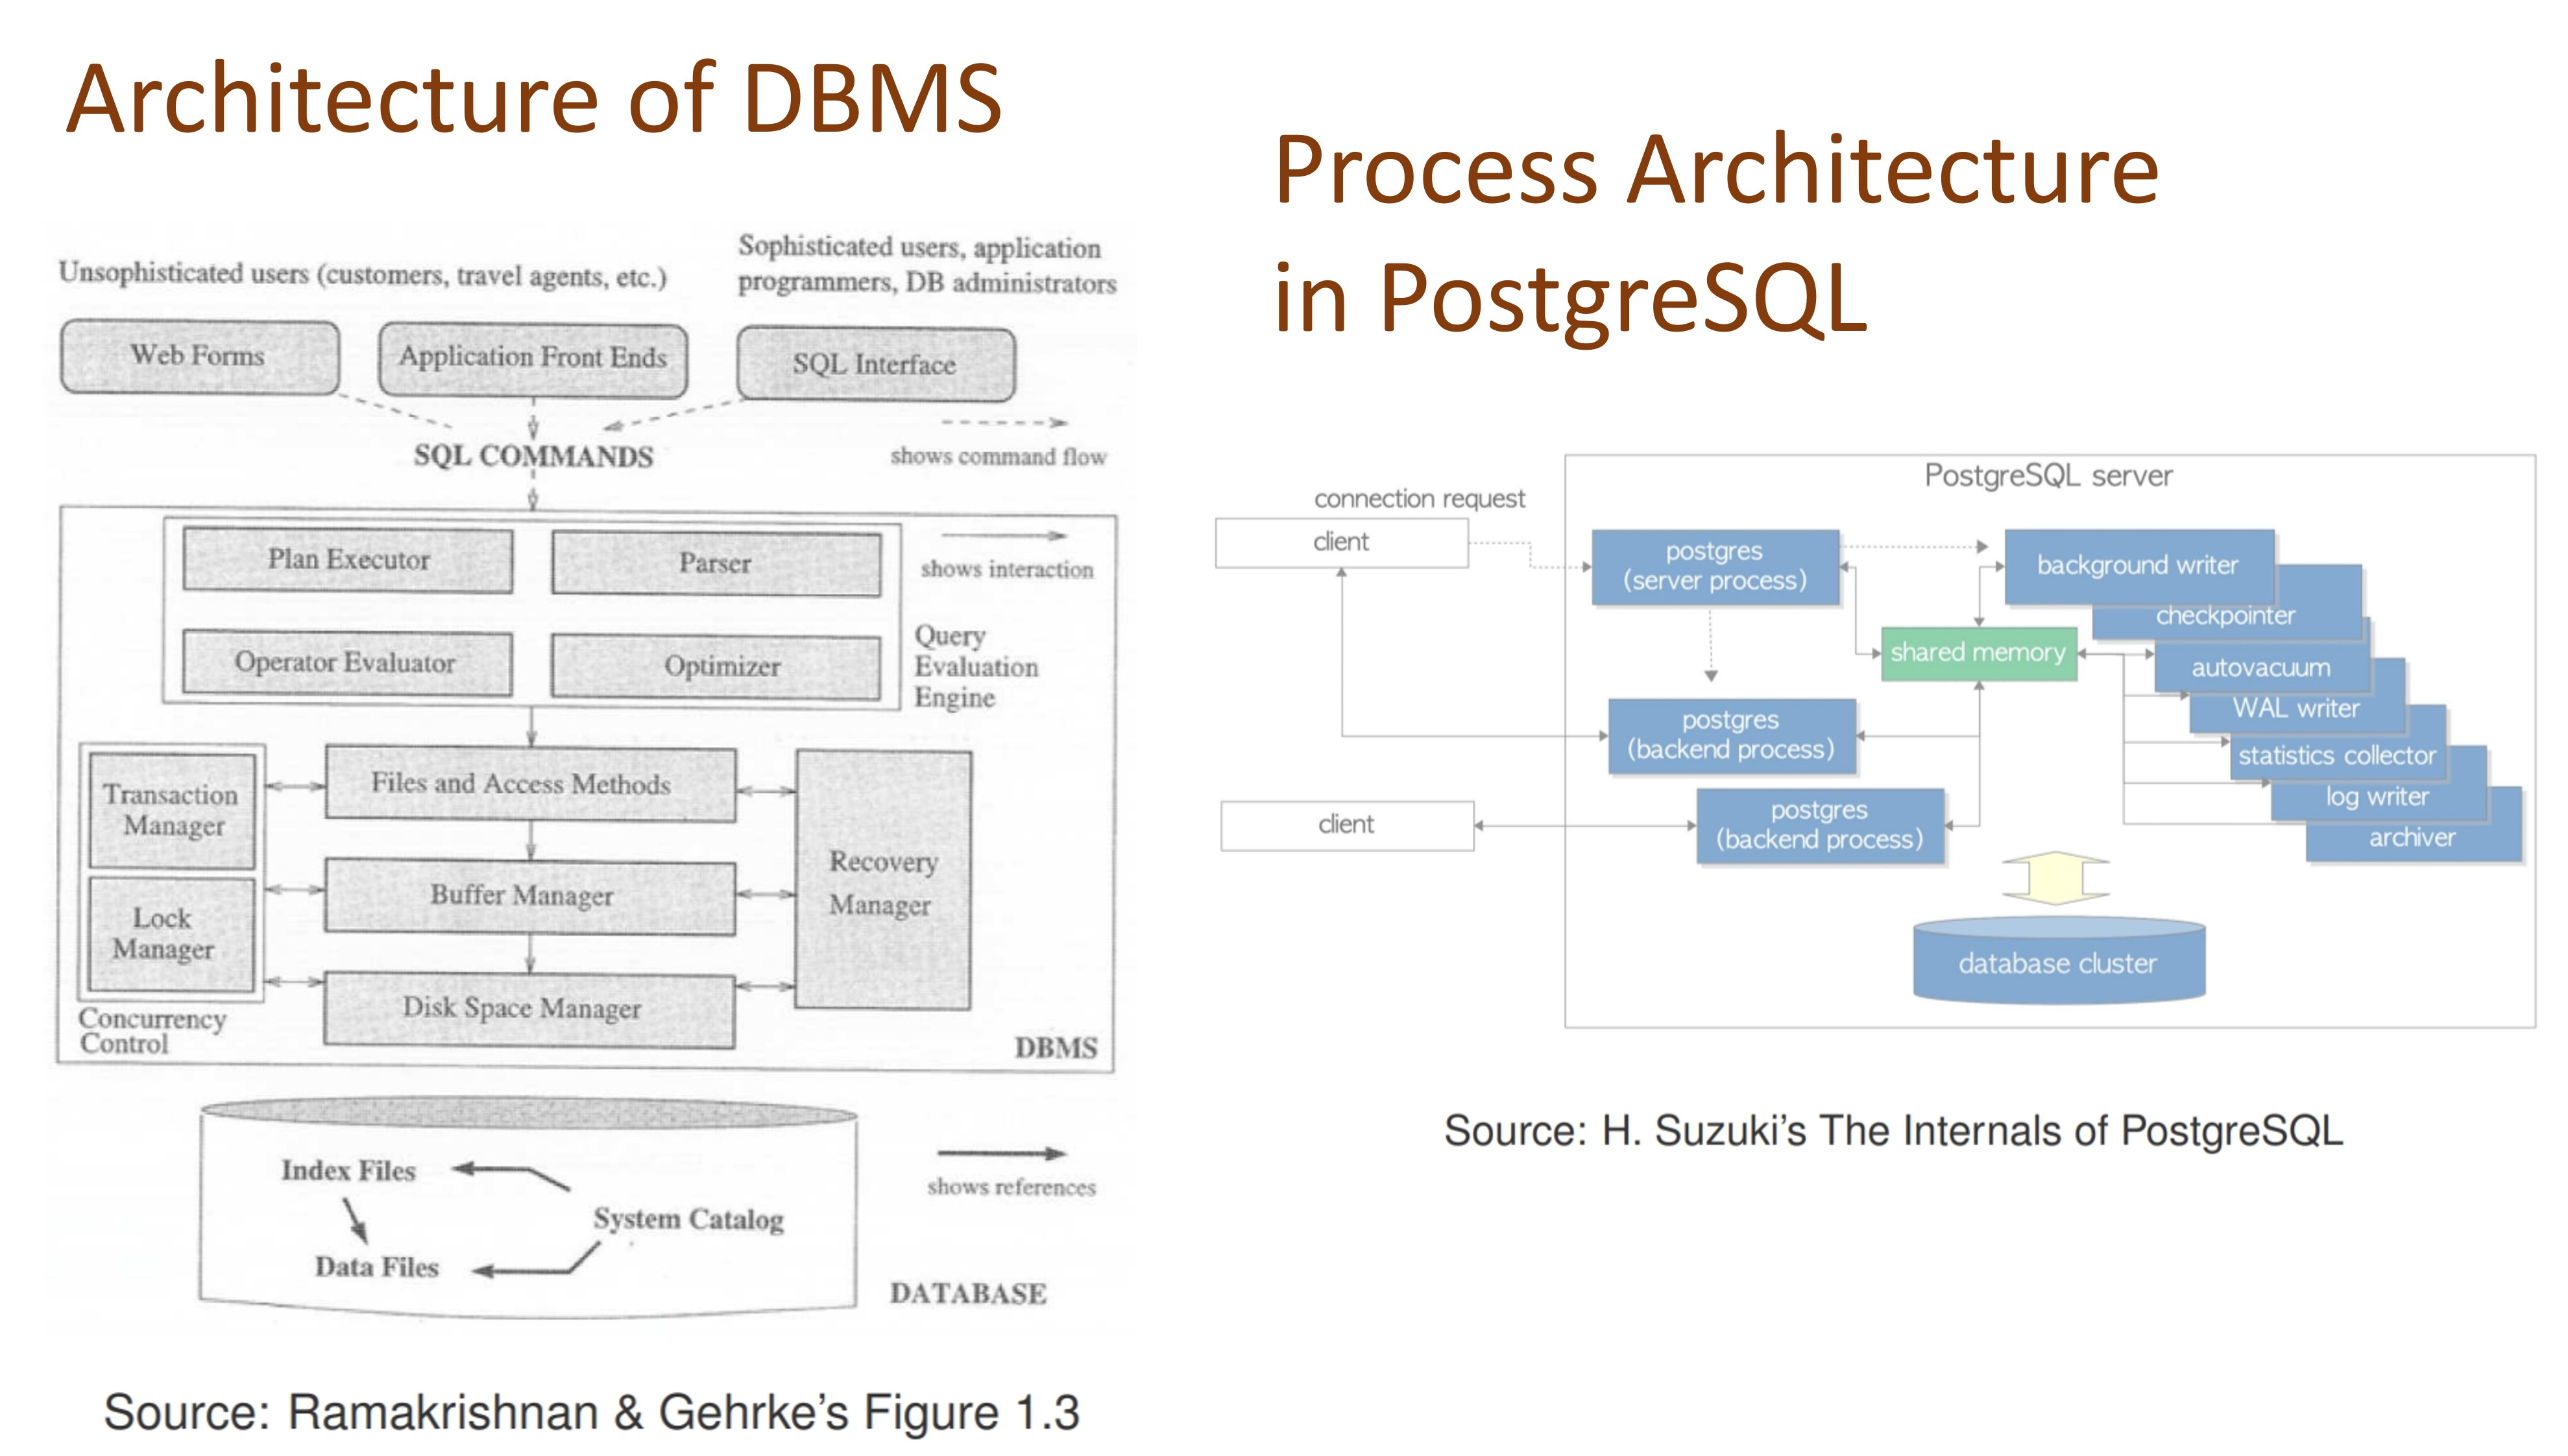
\includegraphics[width = 0.9\linewidth]{DBMSArchitecture}}

\begin{itemize}
\item OLTP: Online Transaction Processing is a type of data processing that consists of executing a number of transactions occurring concurrently—online banking, shopping, order entry, or sending text messages, for example.
\item OLAP: Online Analytical Processing.
\item Focusing on centralized database running on a single server.
\end{itemize}

\section{1. Data Storage}
\textbf{References}: R\&G Chapt 8. (Storage \& Indexing Overview), Chapt 9. (Storing Data: Disks and Files).

\subsubsection{A DBMS stores}
\begin{itemize}
\item Relations (Actual tables)
\item System catalog (aka data dictionary) storing metadata about relations.  \\
(Relation schemas, structure of relations, constraints, triggers. View definitions, Indexes - derived info to speed up access to relations, Statistical information about relations for use by query optimizer.) 
\item Log files: Information maintained for data recovery.
\end{itemize}

\subsubsection{DBMS Storage}
\textbf{Memory Hierarchy}: Primary (registers, RAM), secondary (HDD, SSD), tertiary memory with capacity / cost / access speed / volatility tradeoffs.
\begin{itemize}
\item DBMS stores data on non-volatile disk for persistence.
\item DBMS processes data in main memory (RAM).
\item Disk access operations (I/O). Read: transfer data from disk to RAM. Write: transfer data from RAM to disk.
\item Make use of index to speed up access, so that don't have to retrieve all the data when you run a query. Retrieve index and read only the block that contains specified data. Minimize I/O cost.
\end{itemize}

\subsubsection{Magnetic Hard-Disk Drive HDD}
\centerline{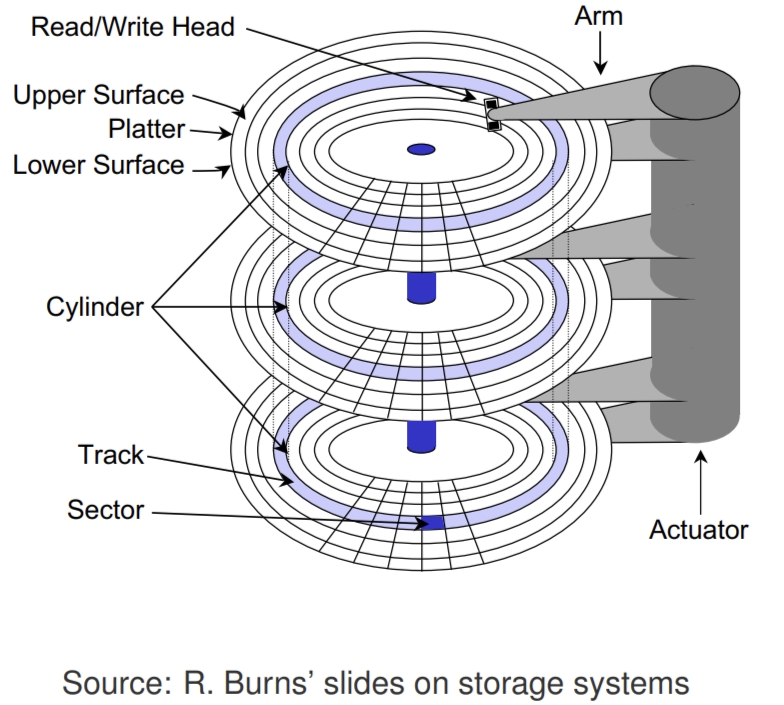
\includegraphics[width = 0.5\linewidth]{HDD}}
\begin{itemize}
\item Cylinder, Track, Sector: Units of the HDD storage system. To read from different tracks, need to move the mechanical HDD arm.
\item \textbf{Disk Access Time}:
	\begin{itemize}
		\item command processing time: interpreting access command by disk controller.
		\item seek time: moving arms to position disk head on track.
		\item rotational delay: waiting for block to rotate under head.
		\item transfer time: actually moving data to/from disk surface.
		\item \textbf{access time = seek time + rotational delay + transfer time. (CPT considered negligible). }
	\end{itemize}
\centerline{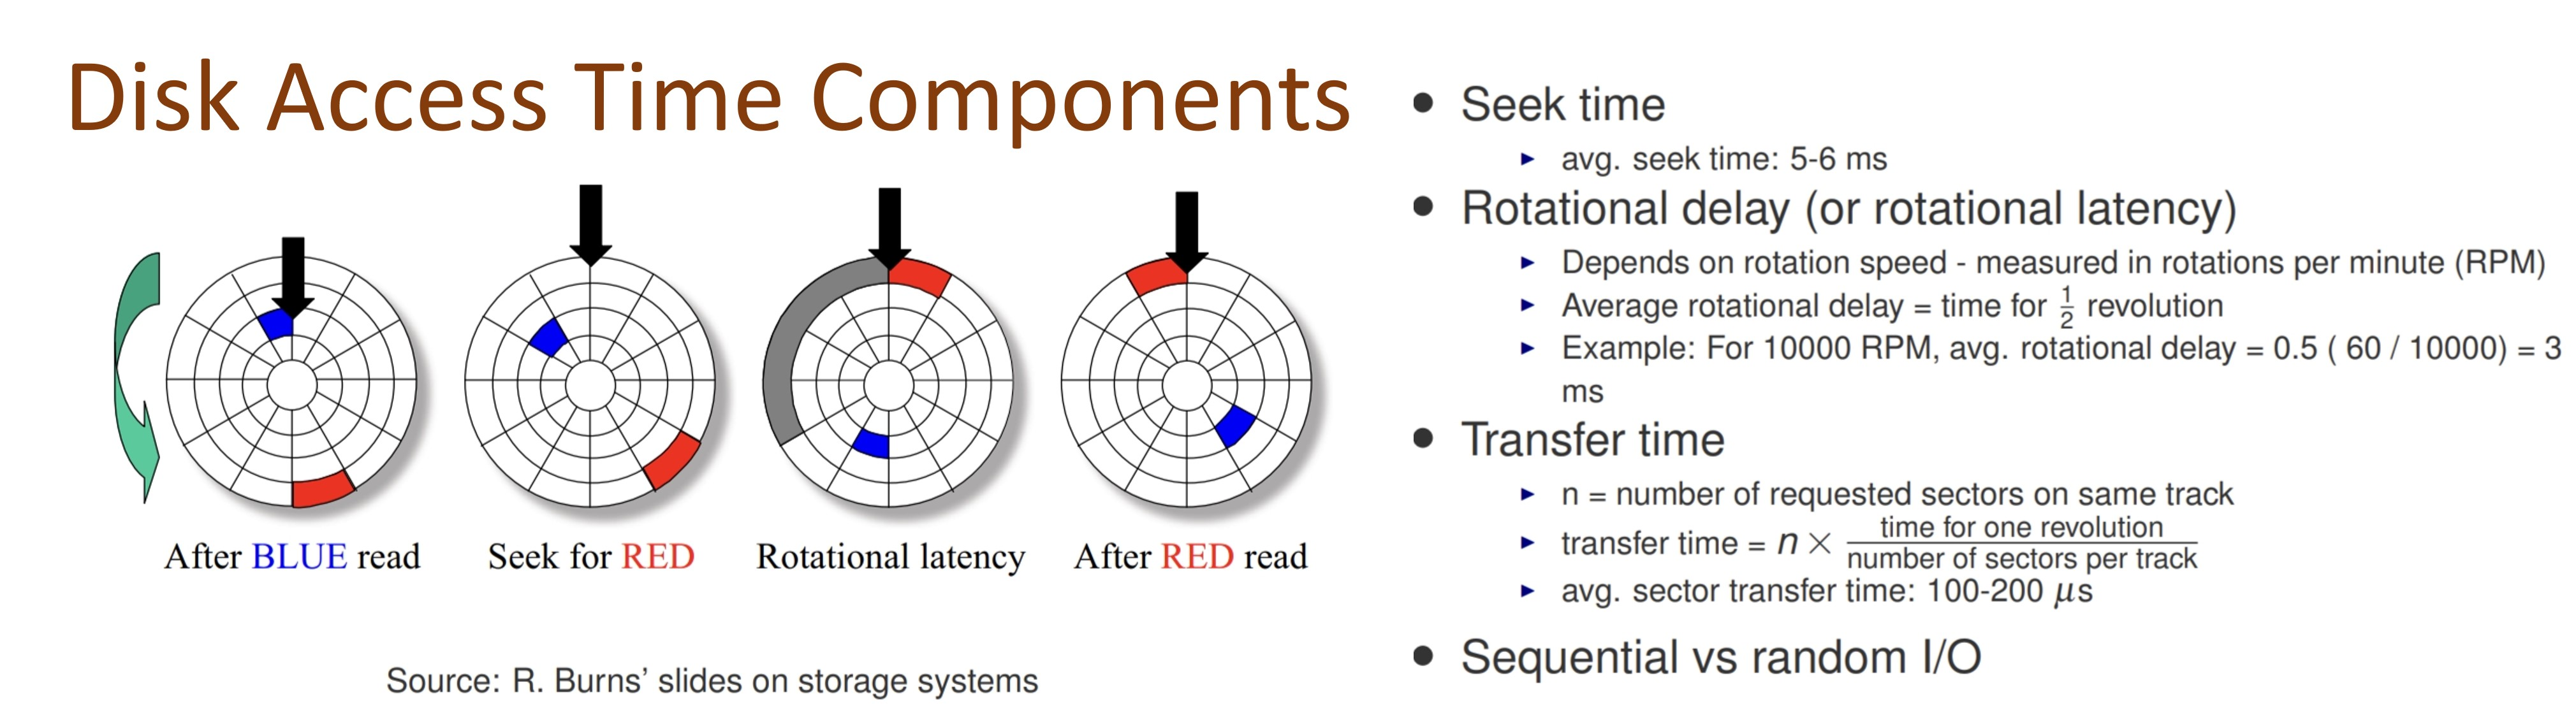
\includegraphics[width = 1\linewidth]{diskAccessTime}}
\item \textbf{Concept of Sequential vs random I/O.} \\
- \textbf{Sequential:} Both sector on same track. \\
- \textbf{Random:} Sectors on different track, require seeking (moving arm).
\item Given a set of data, we hope to store the data contiguously, on the same track. (Minimize incurring random I/O). If data is too large, store on same track, but different surface (aka same cylinder).
\item Complexity hidden to OS by disk controller. Shown as a sequence of memory locations.
\end{itemize}

\subsubsection{Solid-State Drive: SSD}
\begin{itemize}
\item Build with NAND flash memory without any mechanical moving parts. Lower power consumption.
\item \textbf{Random I/O}: 100x faster than HDD. (no moving parts)
\item \textbf{Sequential I/O}: slightly faster than HDD (~ 2x)
\item \textbf{Disadvantages}: update to a page requires erasure of multiple pages (~ 5ms) before ovewriting page. Limited number of times a page can be erased (~ $10^{5} - 10^{6}$)
\end{itemize}

\subsubsection{Storage Manager Components}
\begin{itemize}
\item Data is stored, retrieved in units called \textbf{disk blocks (or pages)}. \\
- Each block = sequence of one or more contiguous sectors.
\item \textbf{Files \& access methods layer (aka file layer)} - deals with organization and retrieval of data.
\item \textbf{Buffer Manager} - controls reading/writing of disk pages.
\item \textbf{Disk Space Manager} - keeps track of pages used by file layer.
\end{itemize}
\centerline{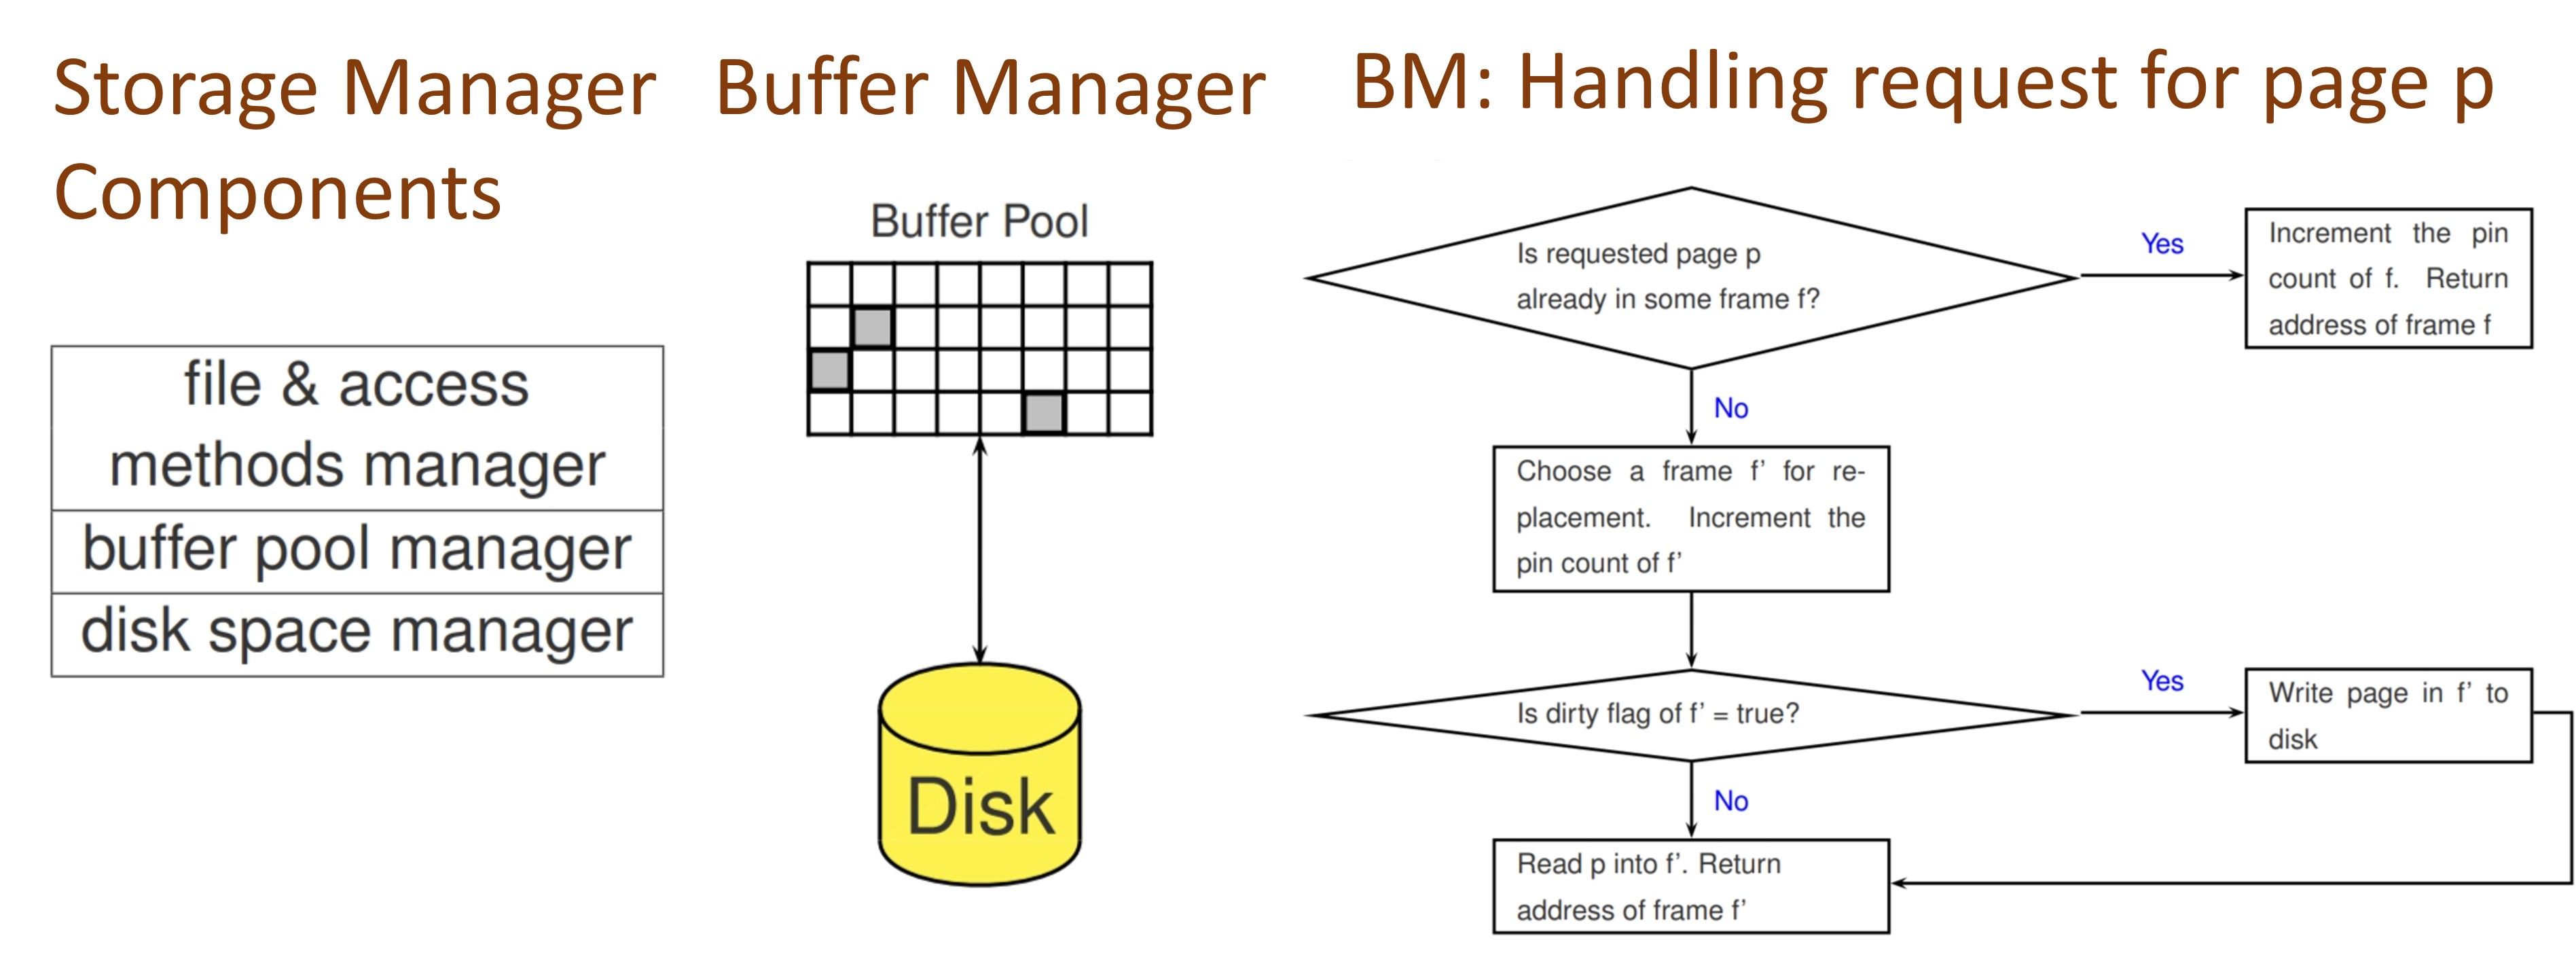
\includegraphics[width = 1\linewidth]{bufferManager}}


\textbf{Buffer Manager}
\begin{itemize}
\item \textbf{Buffer pool}: Main memory allocated for DBMS.
\item Buffer pool is partitioned into block-sized pages called \textbf{frames}.
\item Clients of buffer pool can request for disk page to be fetched into buffer pool, release a disk page in buffer pool.
\item A page in the buffer is \textbf{dirty} if it has been modified \& not updated on disk.
\item \textbf{Two variables} maintained for each frame in buffer pool: 
	\begin{itemize}
		\item \textbf{pin count}: number of clients using page (initialized 0)
		\item \textbf{dirty flag}: whether page is dirty (initialized false)
	\end{itemize}
\item Free list: Keeps track of frames that are free / empty.
\item \textbf{Pin count}: \\
- Incrementing pin count is \textbf{pinning} the requested page in its frame. \\
- Decrementing is \textbf{unpinning} the page. 
	\begin{itemize}
		\item Unpinning a page, dirty flag should be updated to true if page is dirty.
		\item A page in buffer can be replaced only when pin count is 0. 
		\item Before replacing buffer page, needs to be written back to disk if its dirty flag is true. 
	\end{itemize}
\item Buffer manager coordinates with transaction manager to ensure data correctness and recoverability.
\item \textbf{Replacement Policies}
	\begin{itemize}
		\item Replacement policy: Deciding which unpinned page to replace. (some examples:)
		\item Random, FIFO, Most Recently Used (MRU), Least Recently Used (LRU): (Use queue of pointers to frames with pin count = 0), most common, makes use of temporal locality.
		\item \textbf{Clock}: cheaper popular variant of LRU \\
		- \textbf{current} variable: points to some buffer frame. \\
		- Each frame has a \textbf{referenced bit}, turns on when its pin count turns 0. \\
		- Replace a page that has referenced bit off \& pin count = 0.
	\end{itemize}
\centerline{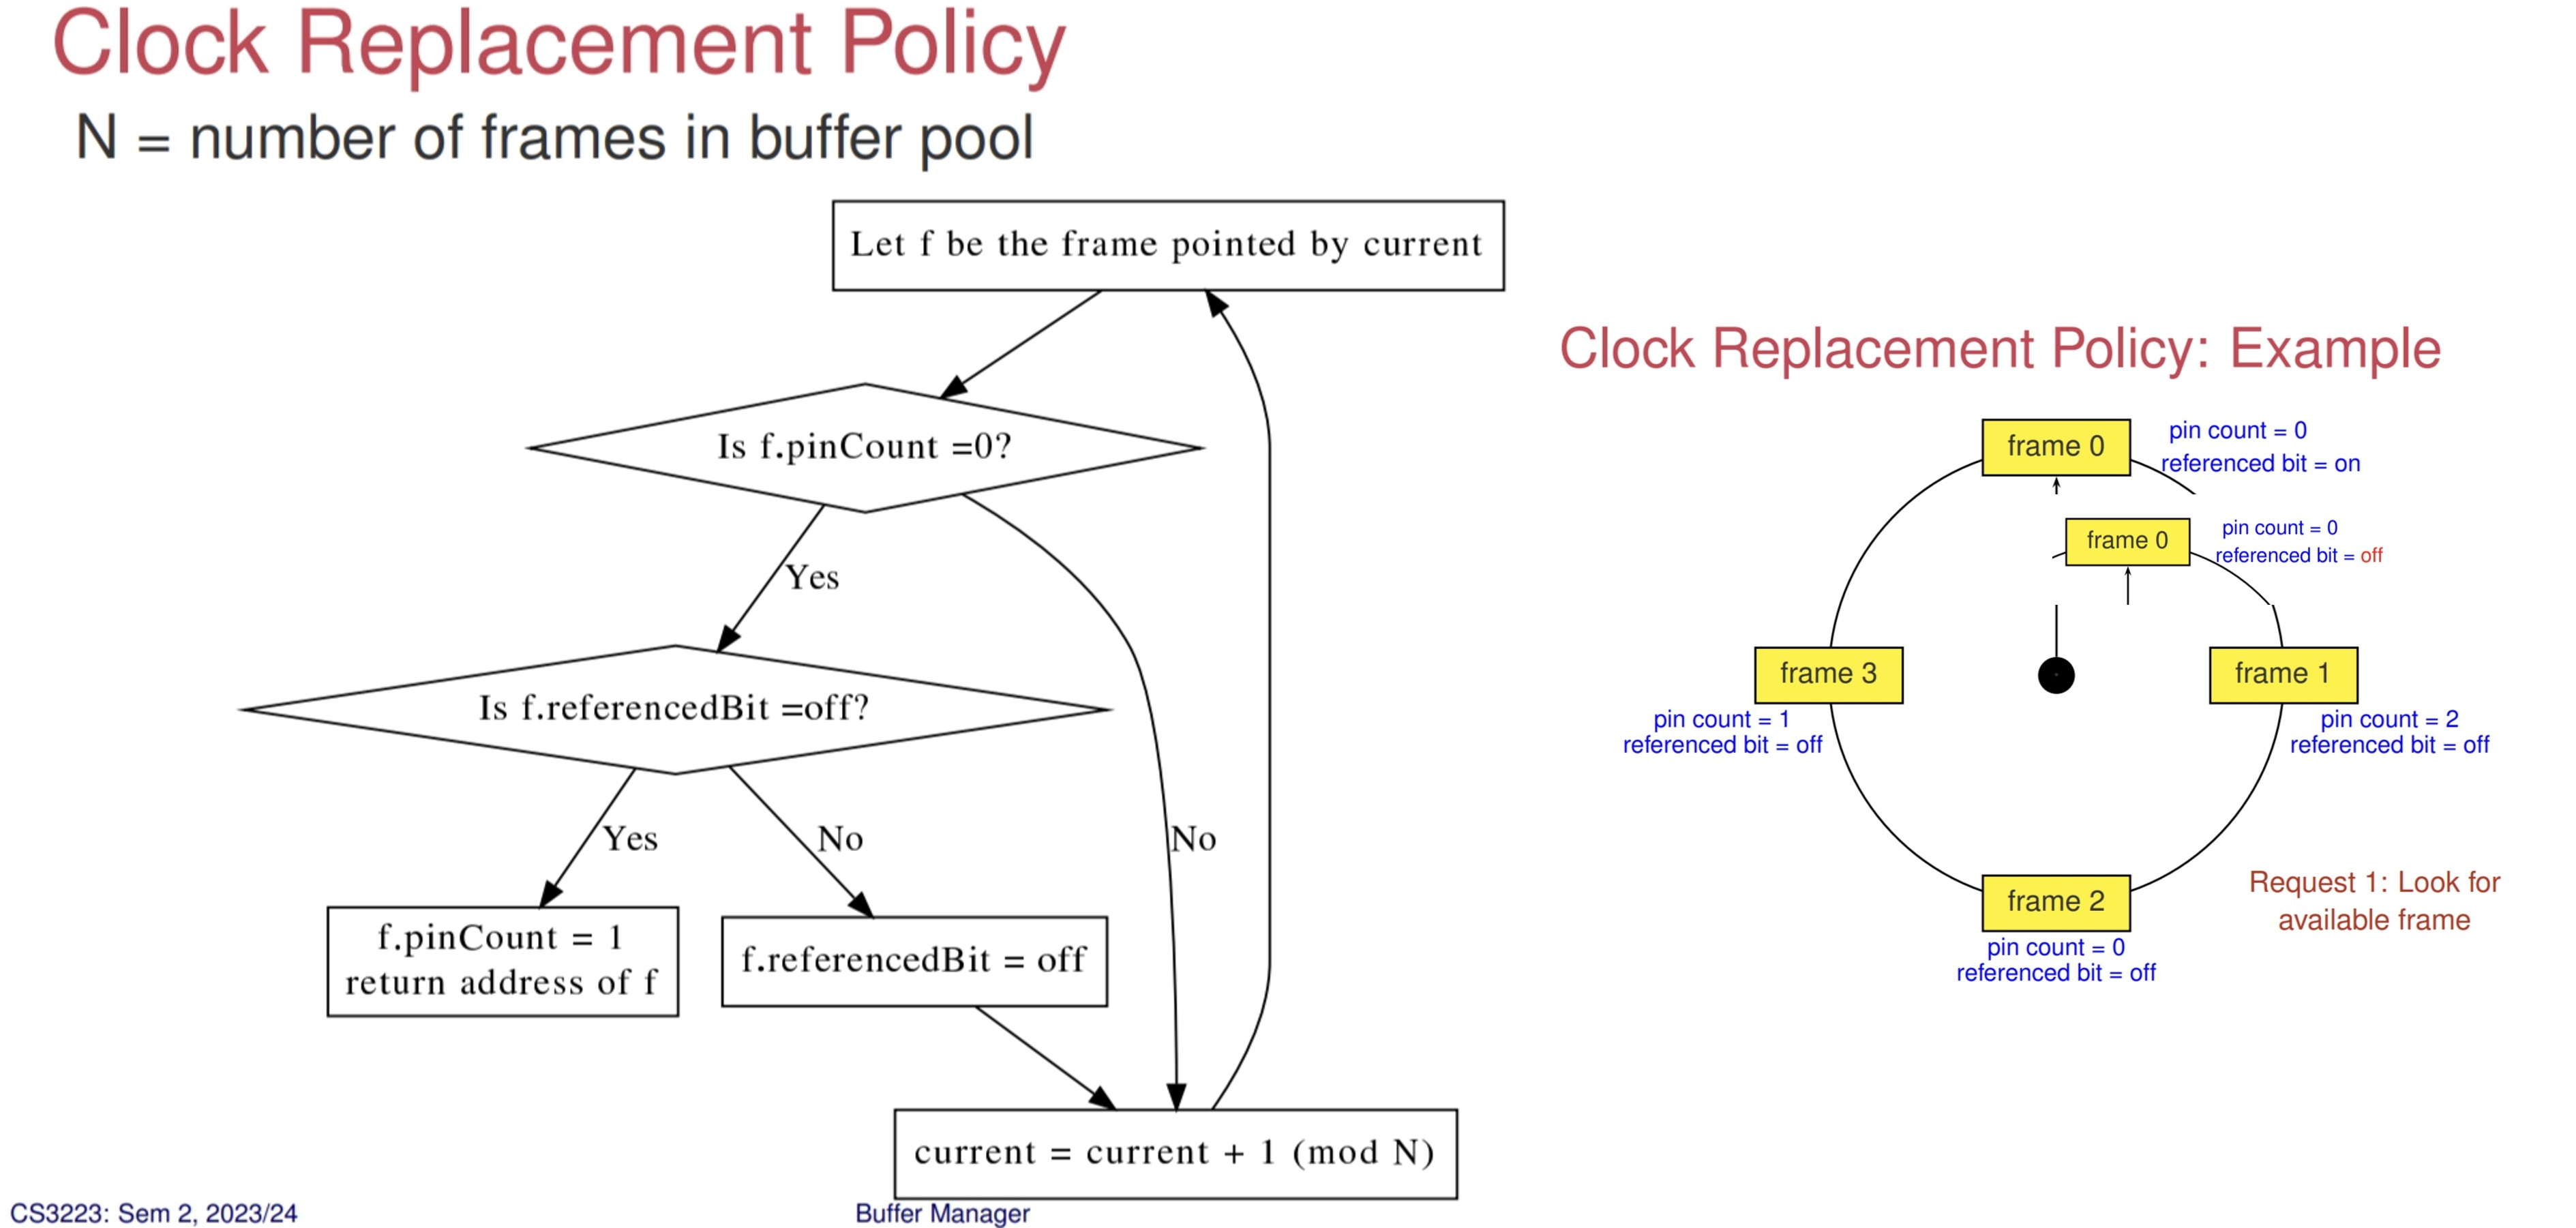
\includegraphics[width = 1\linewidth]{clockReplacementPolicy}}
\end{itemize}

\columnbreak

\subsection{Files}
\textbf{File Abstraction}
\begin{itemize}
	\item Each relation is a file of records.
	\item Each record has a unique record identifier called RID / TID.
	\item Common file operations: create/delete file, insert record, delete/get record with given RID, scan all records.
\end{itemize}
\textbf{File Organization}: Method of arranging data records in a file that is stored on disk.
\begin{itemize}
	\item \textbf{Heap file}: Unordered file
	\item \textbf{Sorted file}: Records order on some search key.
	\item \textbf{Hashed file}: Records located in blocks via a hash function.
\end{itemize}

\subsubsection{Heap File Implementations}
\centerline{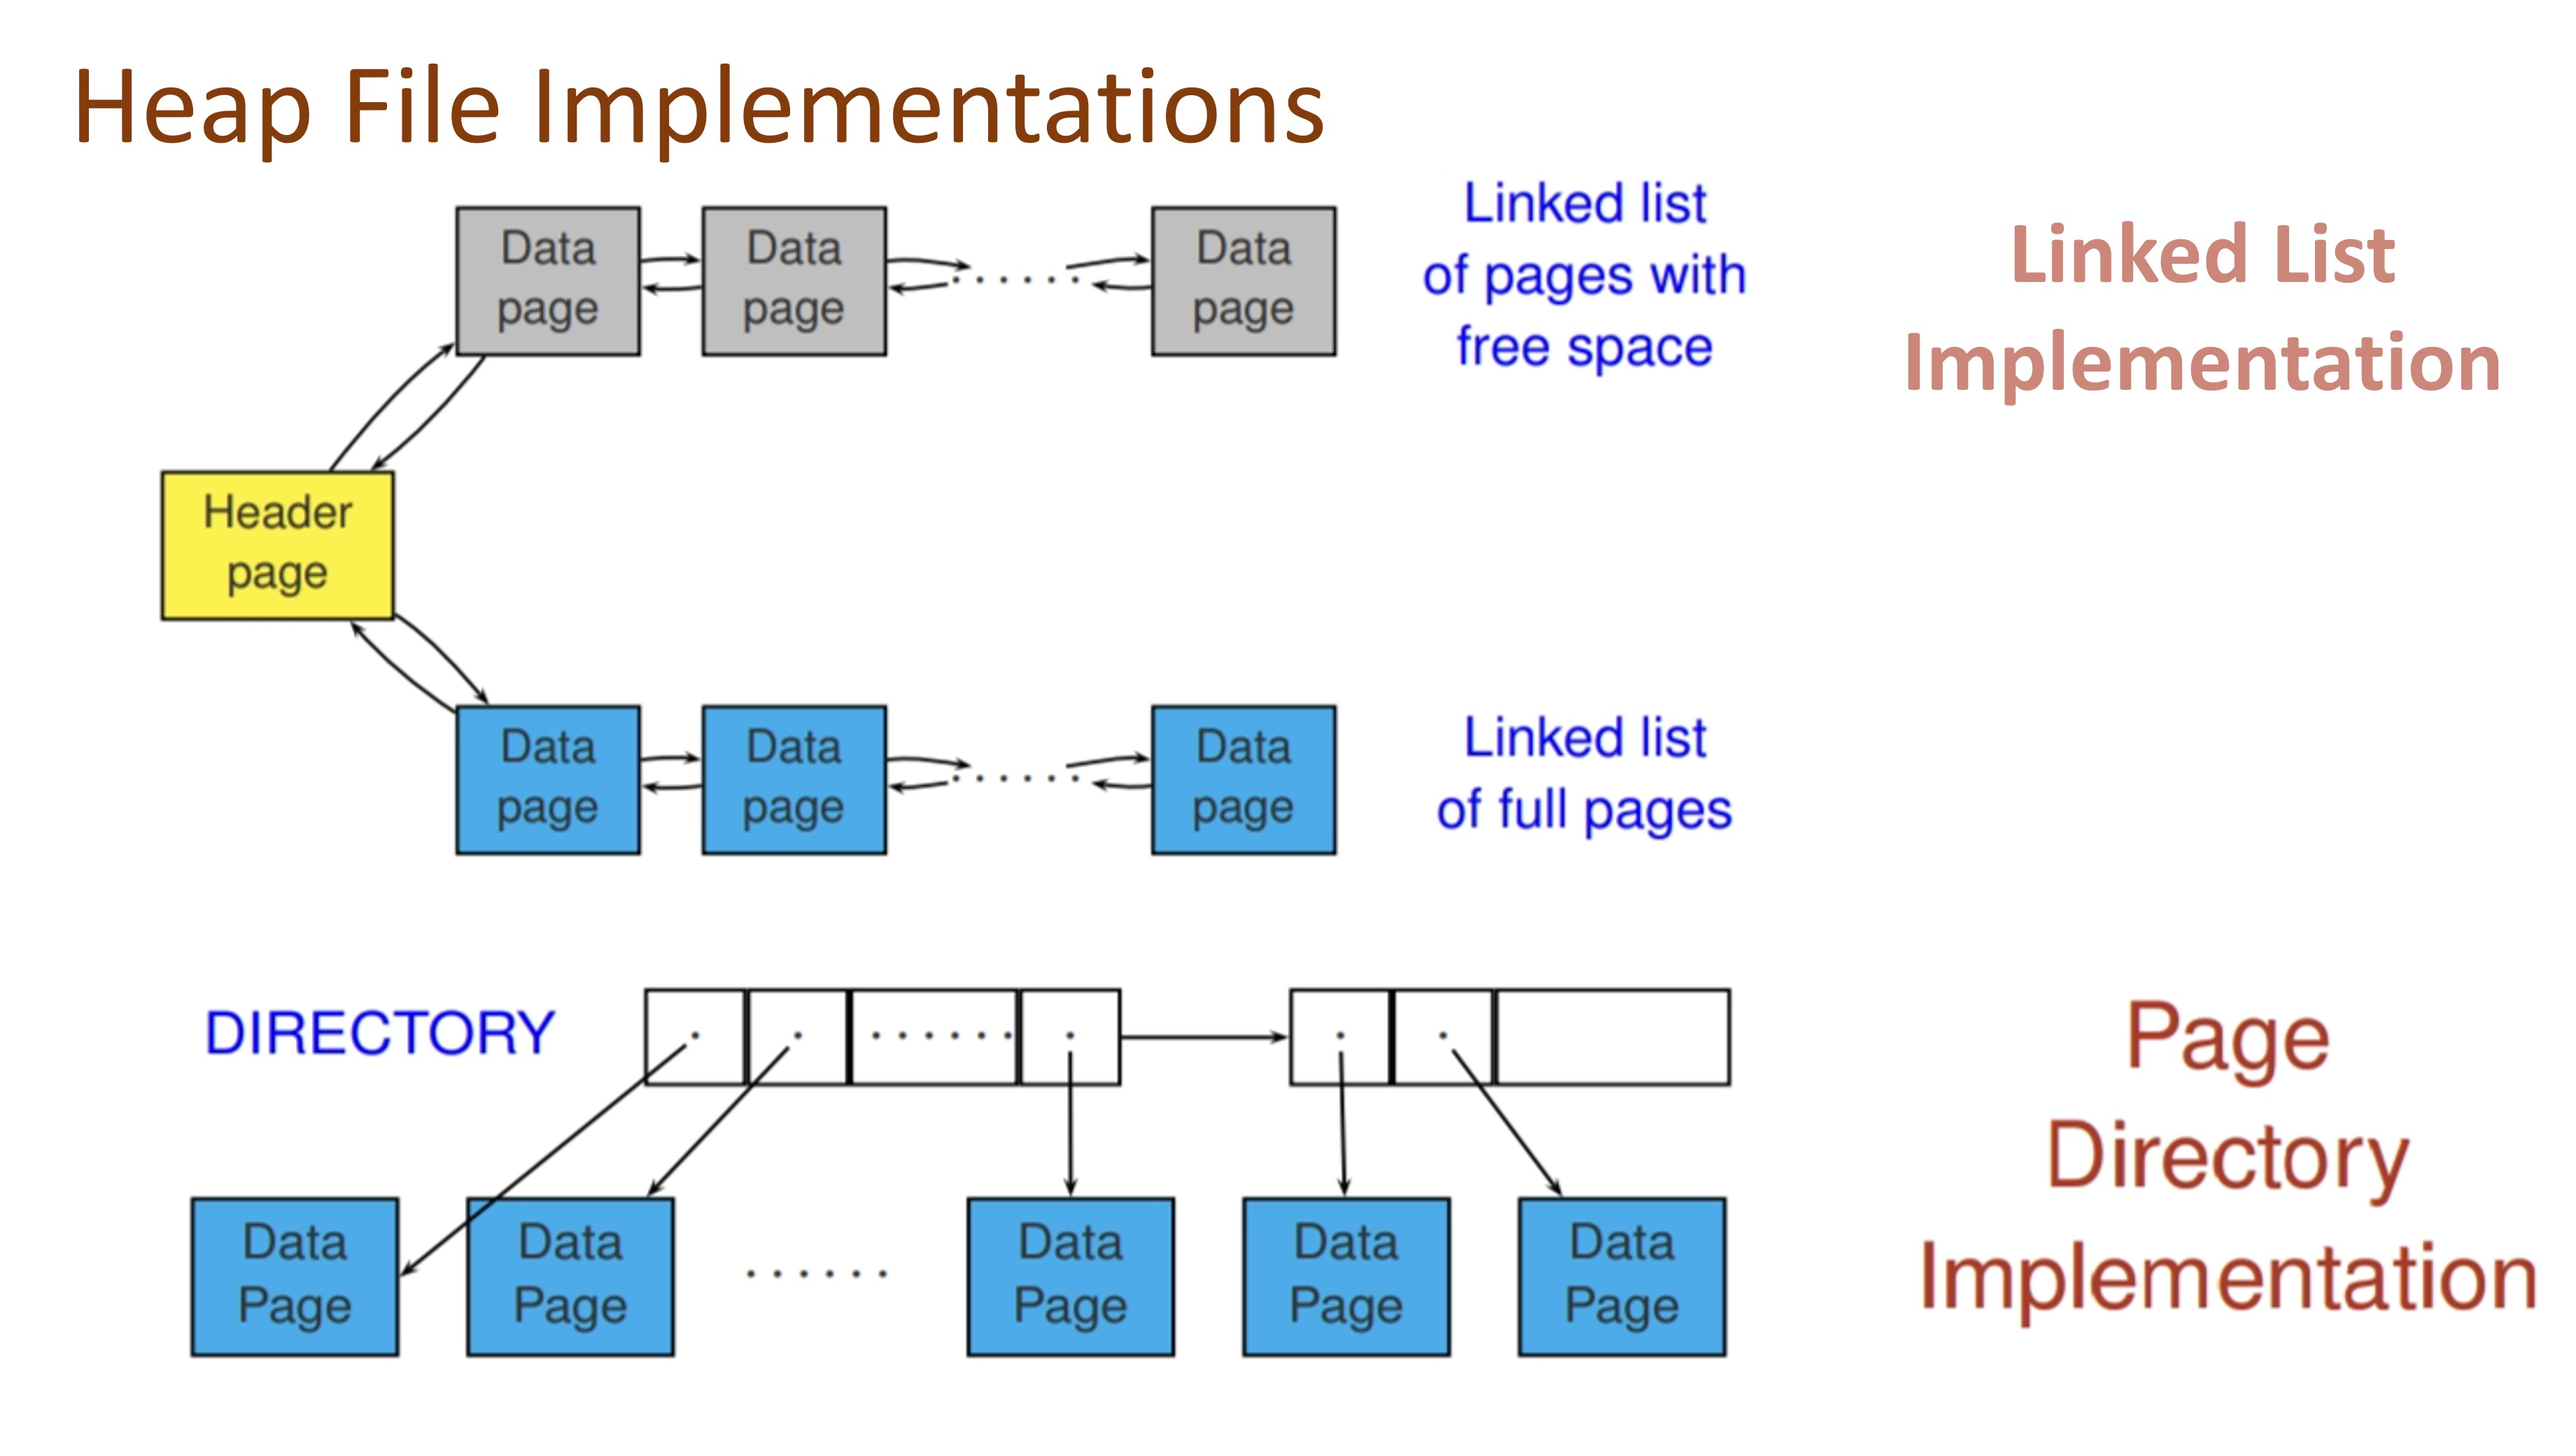
\includegraphics[width = 0.7\linewidth]{heapFileImplementations}}
\begin{itemize}
\item \textbf{Linked list implementation}: Two linked lists, one with pages with free space, other of completely full pages.
\item \textbf{Page Directory Implementation}: Two leveled implementation. Each big block is a disk block with some metadata. Each disk block has a number of data pages.
\end{itemize}

\textbf{Page Formats}: \\
Records are organized within a page and referenced with the RID.
\begin{itemize}
\item \textbf{RID = (page id, slot number)}
\item For \textbf{Fixed-Length Records}, Organization can be:
\begin{itemize}
\item \textbf{Packed Organization}: Store records in contiguous slots. 
\item  For packed organization, memory organization is tough and costly when record in slot is deleted, need to move up a record. But as RID serves as a reference, but need to propagate change in RID.
\item \textbf{Unpacked Organization}: Uses bit array to maintain free slots.
\item For unpacked organization, more bookkeeping needed (use bitmap, 1 \& 0 to check if occupied) to store records.
\end{itemize}
\item For \textbf{Variable-Length Records}: We could assume some maximum size, then use packed organization. But wasteful. Instead, we can use \textbf{Slotted Page Organization}.
\end{itemize}
\centerline{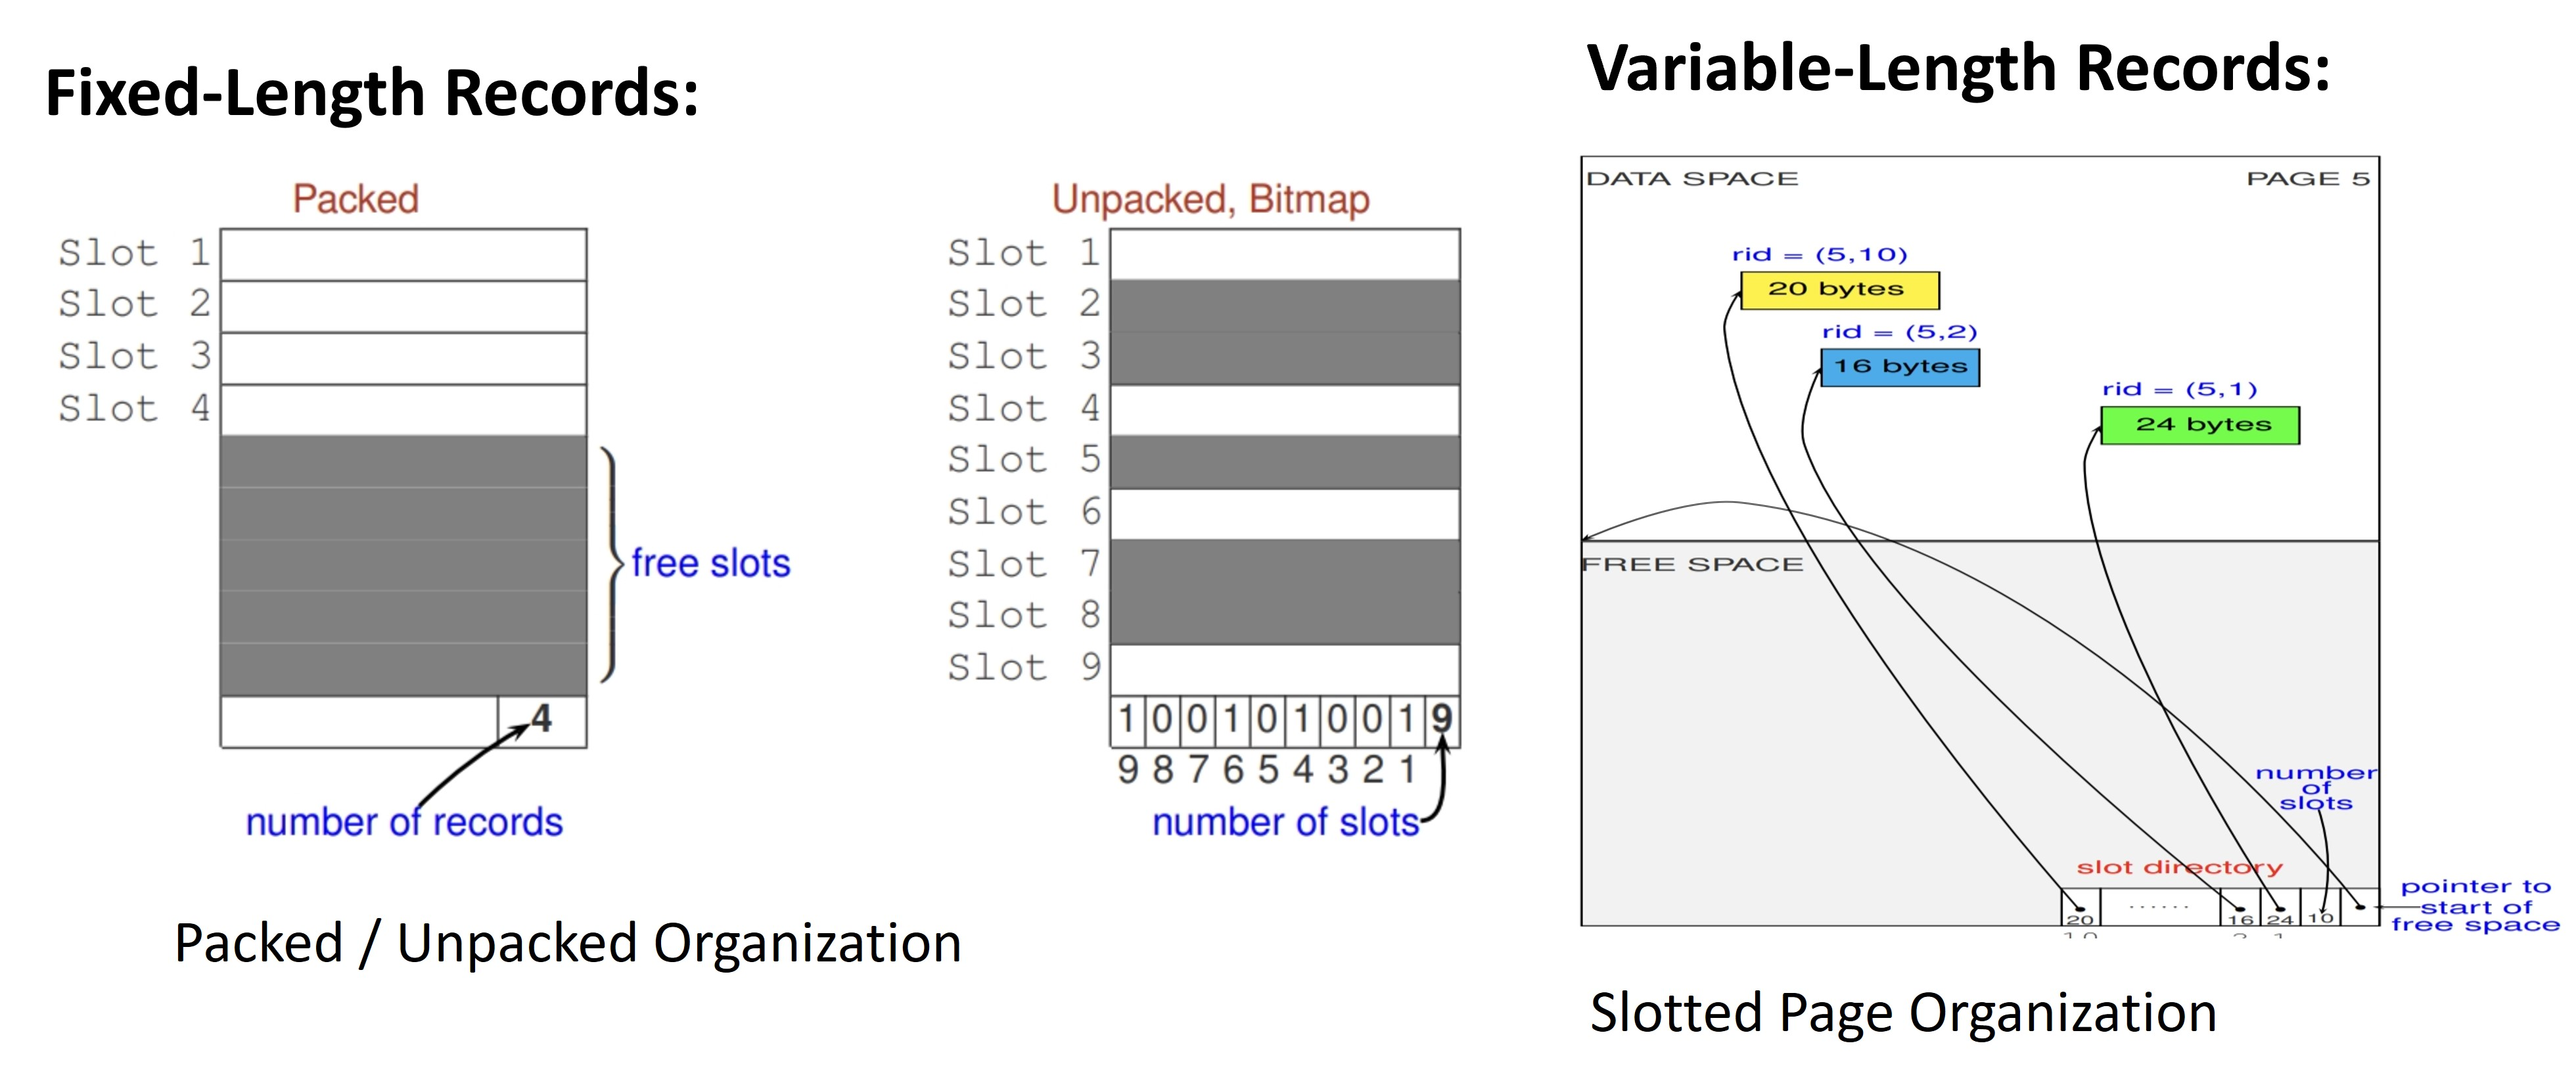
\includegraphics[width = 1\linewidth]{pageFormats}}

\centerline{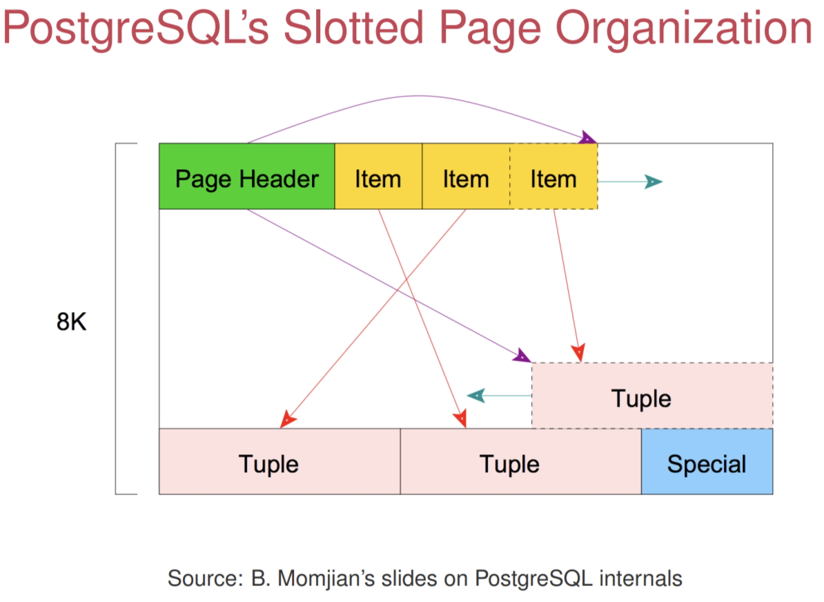
\includegraphics[width = 0.7\linewidth]{PostgreSQLPageOrg}}
\textbf{Record Formats}: Organizing fields within a record. \\
\medskip
\centerline{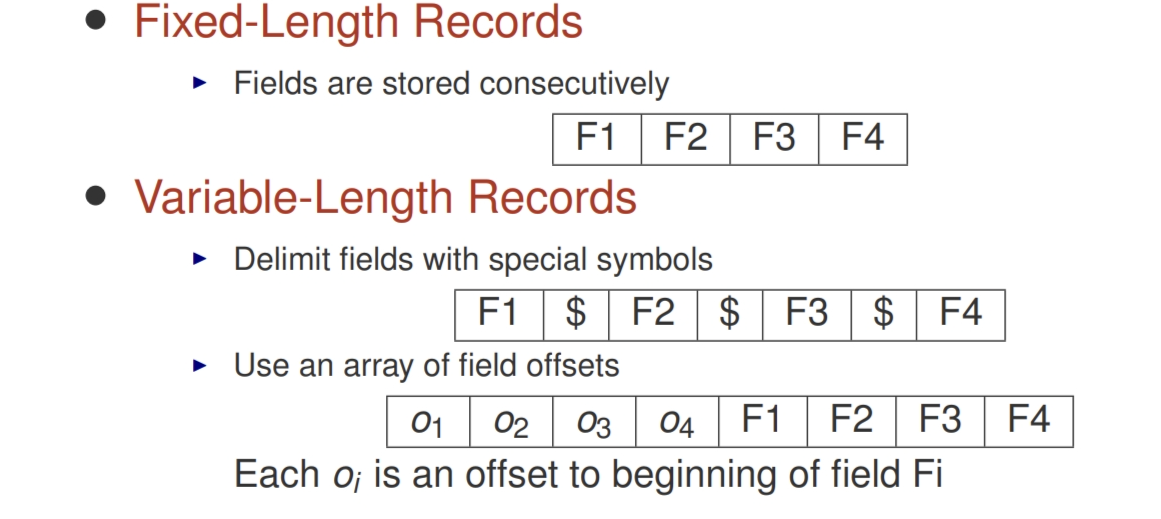
\includegraphics[width = 0.8\linewidth]{recordFormats}}

\section{2. Indexing}
Need some auxiliary data structure to make efficient queries.

\subsection{Index}
\begin{itemize}
\item An \textbf{index} is a data structure to speed up retrieval of data records based on some search key.
\item A \textbf{search key} is a sequence of $k$ data attributes, $k \geq 1$. (A search key is aka \textit{composite search key} if $k > 1$, e.g. (state, city).)
\item An index is a \textbf{unique index} if search key is a candidate key, otherwise it is \textbf{non-unique index}.
\item An index is stored as a file, records in index file referred to as \textbf{data entries}.
\end{itemize}
\centerline{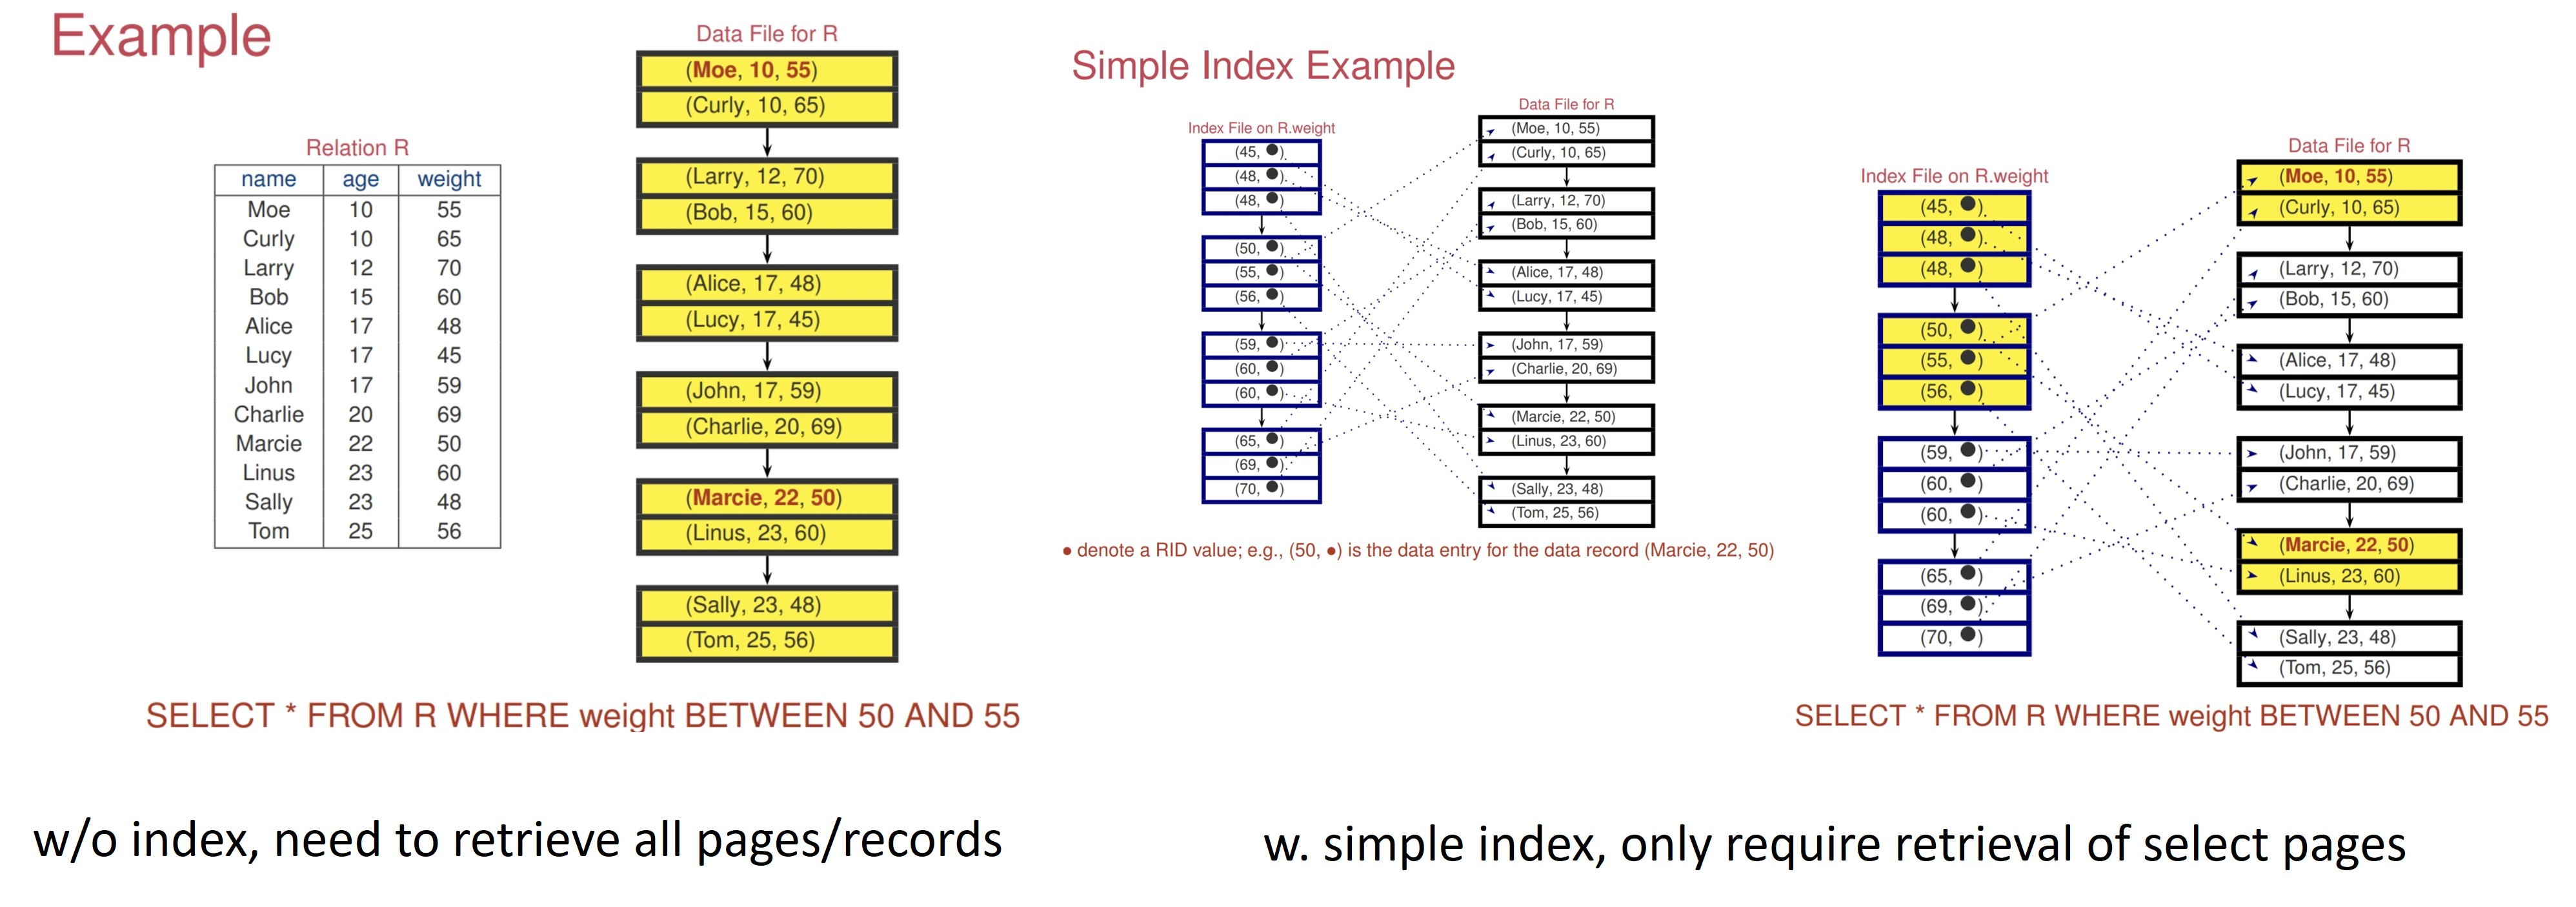
\includegraphics[width = 1\linewidth]{simpleIndex}}

\subsection{Index Types}
Two main types of indexes
\begin{itemize}
\item \textbf{Tree-based Index}: Based on sorting of search key values (E.g. ISAM, $B^+$-tree)
\item \textbf{Hash-based Index}: Data entries accessed using hashing function (E.g. static/ extendible / linear hashing)
\item Considerations when choosing an index: 
	\begin{itemize}
	\item Search Performance \\ 
	(Equality search: $k=v$, use hash-based.) (Range search, use tree)
	\item Storage overhead
	\item Update performance
	\end{itemize}
\end{itemize}

\subsection{Tree-based Indexing: $B^+$-Tree}
$B^+$ tree is a dynamic structure that adjusts to changes in the file gracefully, most widely used index structure as it adjusts well to changes and supports both equality and range queries.
\begin{itemize}
\item \textbf{Balanced tree}: Operations (insert, delete) on tree keep it balanced.
\item \textbf{Internal nodes} direct the search.
\item \textbf{Leaf nodes} contain the data entries. Leaf pages linked using page pointers for easy traversal of sequence of leaf pages in either direction.
\item \textbf{Value $d$} is parameter of $B^+$-tree, called order of the tree, is a measure of capacity of a tree node. Each node contains $m$ entries, where $d \leq m \leq 2d$, except root node, where $1 \leq m \leq 2d$
\end{itemize}


\subsection{$B^+$-tree Index}
\centerline{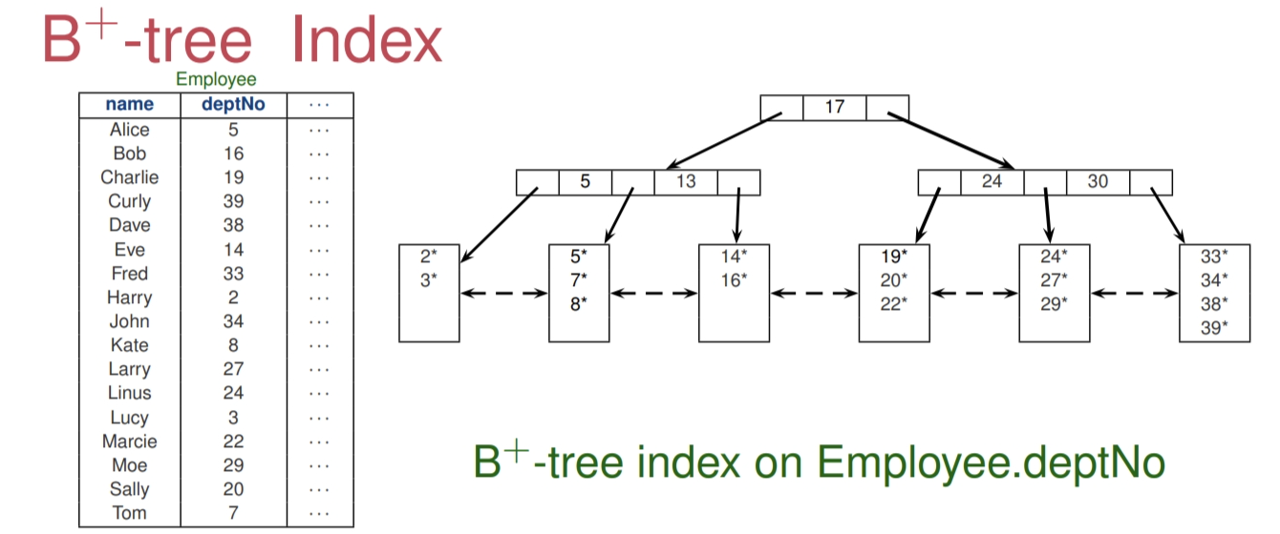
\includegraphics[width = 1\linewidth]{B+TreeIndex}}
\begin{itemize}
\item Each node is either a \textbf{leaf node} (bottom-most level) or an internal node. 
\item Top-most internal node is the \textbf{root node} located at \textbf{level 0}.
\item \textbf{Height of Tree} = number of level of internal nodes. (Leaf nodes are at level $h$ where $h$ = height of tree).
\item Nodes at same level are \textbf{sibling nodes} if they have the same parent node.
\item \textbf{Leaf Nodes}:
	\begin{itemize}
	\item Leaf nodes store sorted data entries.
	\item $k*$ denote data entry of form (k, RID), where k = search key value of corresponding data record, RID = RID of data record.
	\item Lead nodes are doubly-linked to adjacent nodes.
	\end{itemize}
\item \textbf{Internal Nodes}:
	\begin{itemize}
	\item Internal nodes store index entries of the form (p: pointer, k: separator)\\
	 $(p_0, k_1, p_1, k_2, p_2, ..., p_n)$
	\item $k_1 < k_2 < ... < K_n$
	\item Each $(k_i, p_i)$ is an \textbf{index entry}, $k_i$ serves as \textbf{separator} between node contents pointed to by $p_{i-1}$ \& $p_i$
	\item $p_i$ = disk page address (root node of an index subtree $T_i$)
	\end{itemize}
\end{itemize}

\null \null
\columnbreak

\subsection{$B^+$-tree Index Properties}
\centerline{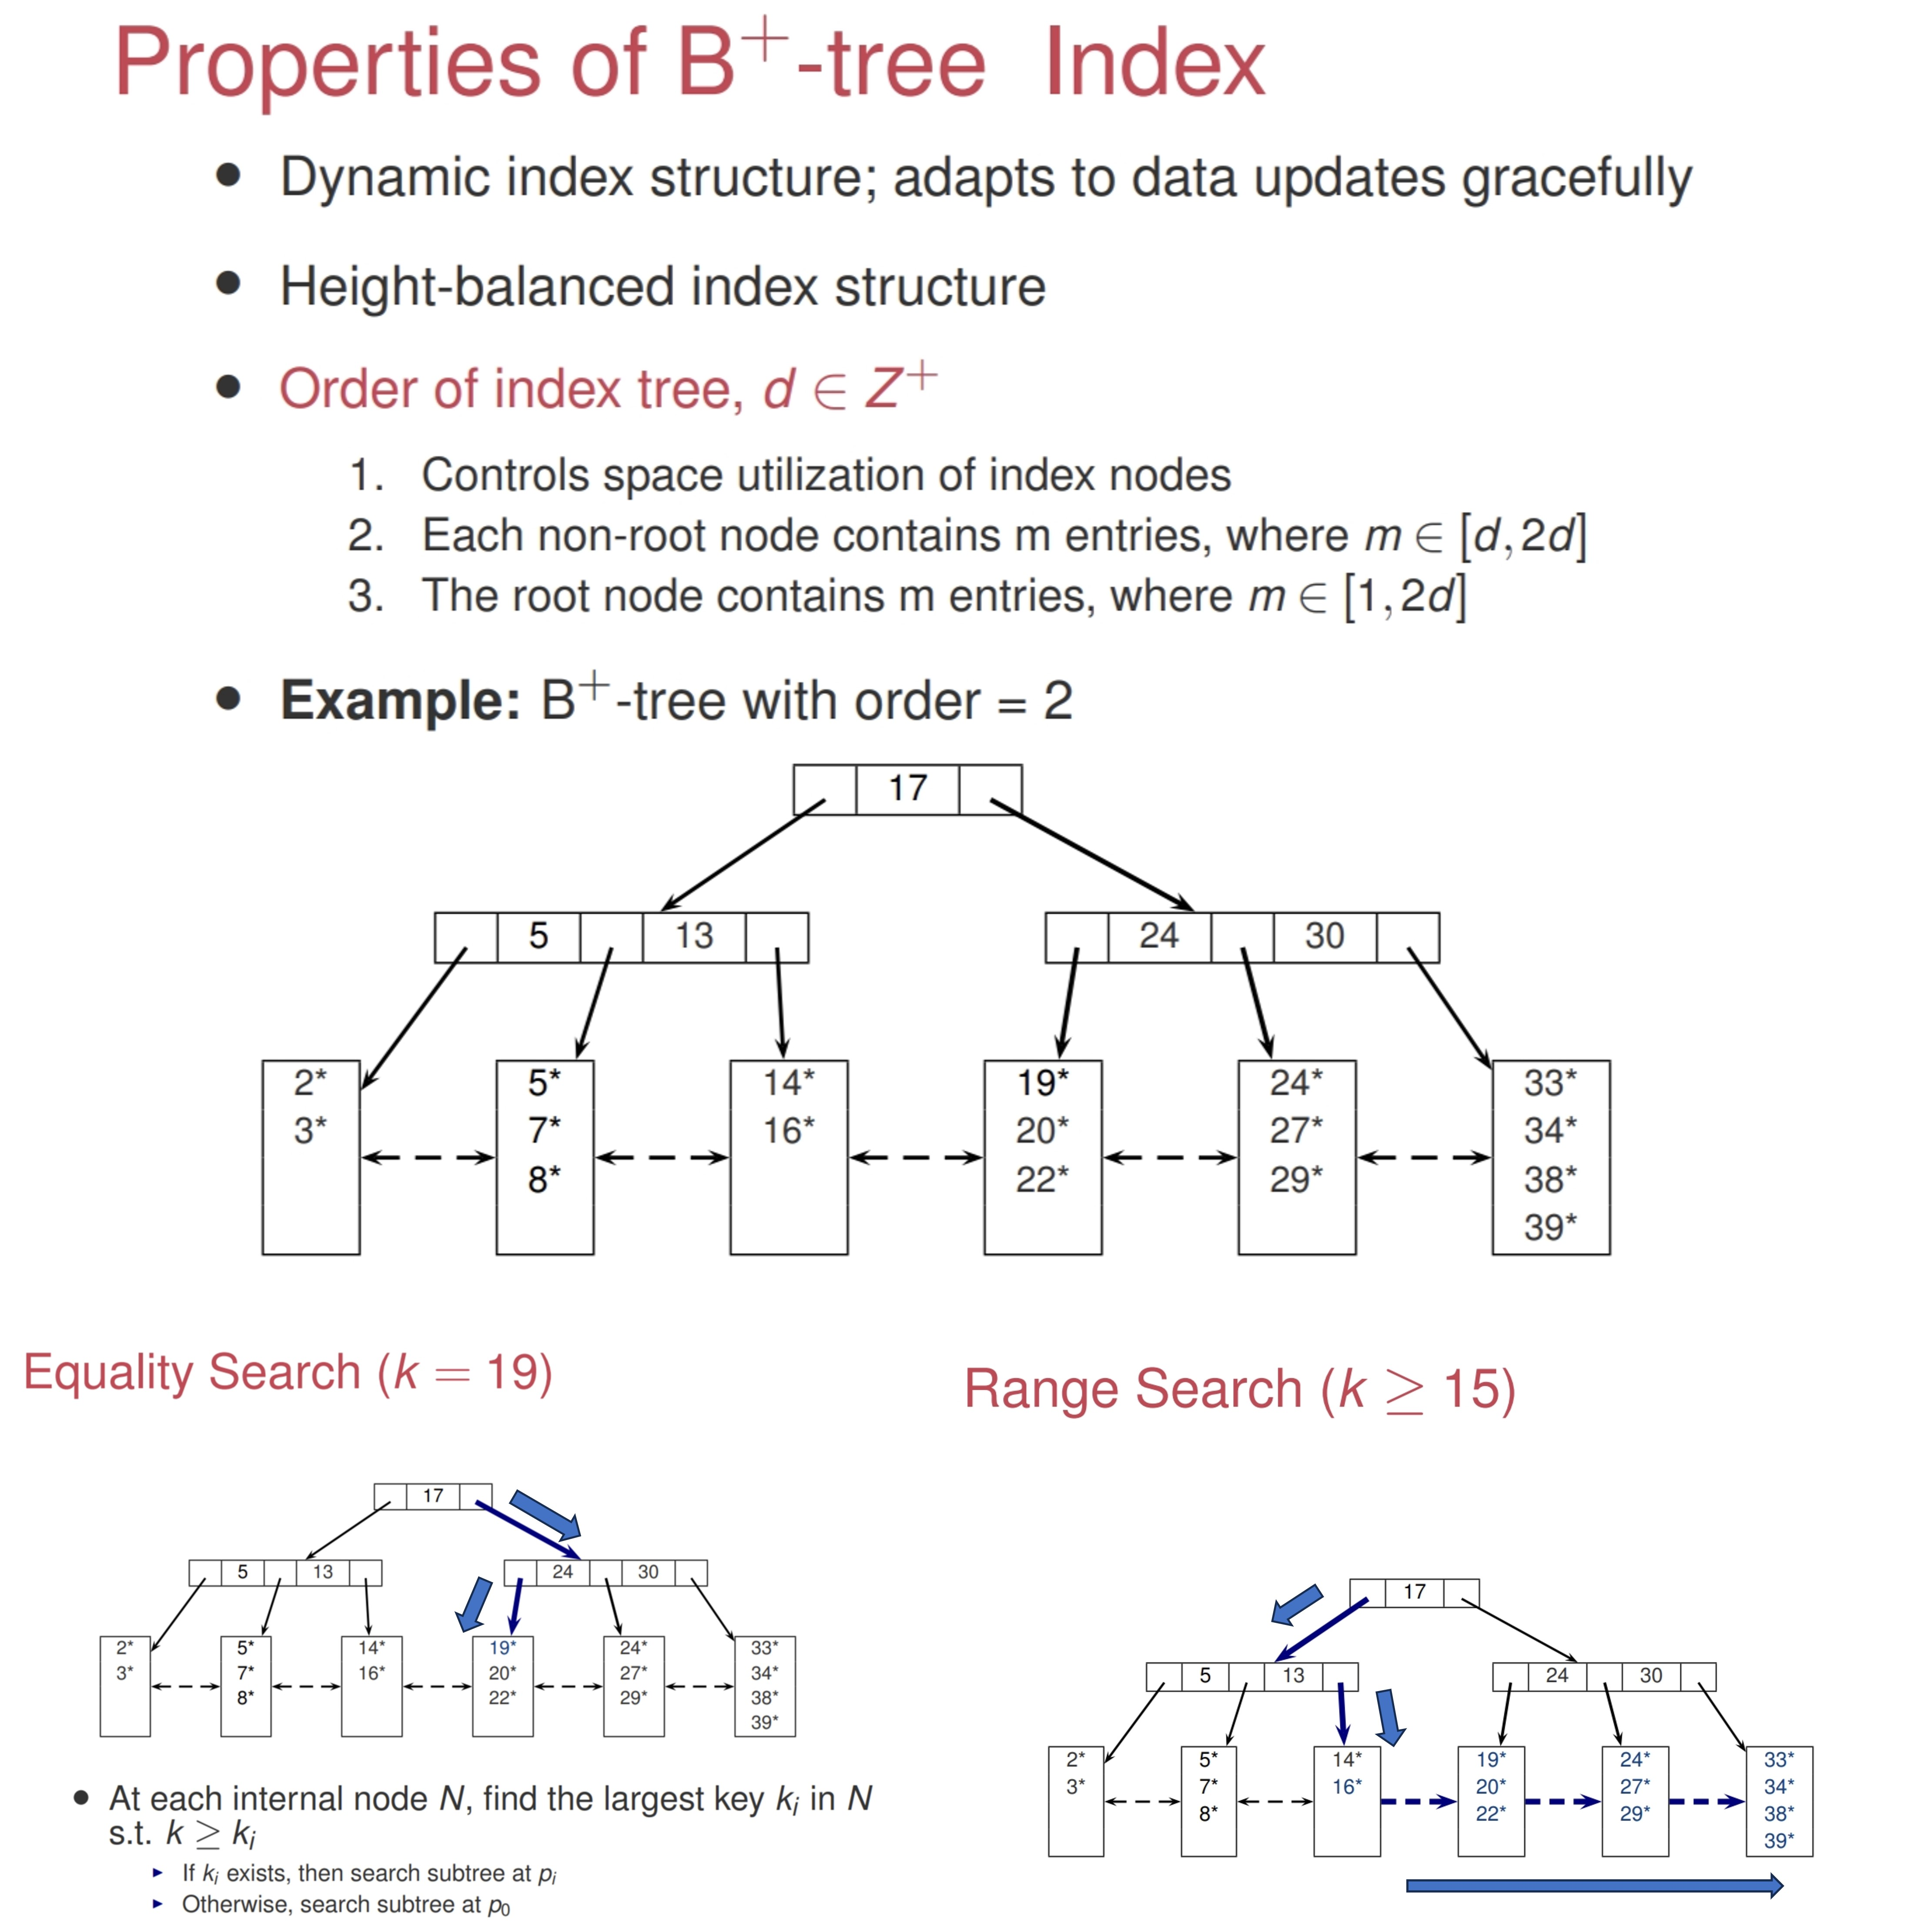
\includegraphics[width = 1\linewidth]{Bproperties}}

\subsubsection{Formats of Data Entries in B-Tree}
\begin{itemize}
\item \textbf{Format 1}: k* is actual \textit{data record} (with search key value $k$)
\item \textbf{Format 2}: k* is of form \textit{(k, rid)}, where rid is record identifier of record with search key value $k$.
\item \textbf{Format 3}: k* is of form \textit{(k, rid-list)}, where rid-list is list of record identifiers of data records with search key value $k$.
\item Note, examples assume Format 2.
\end{itemize}
\centerline{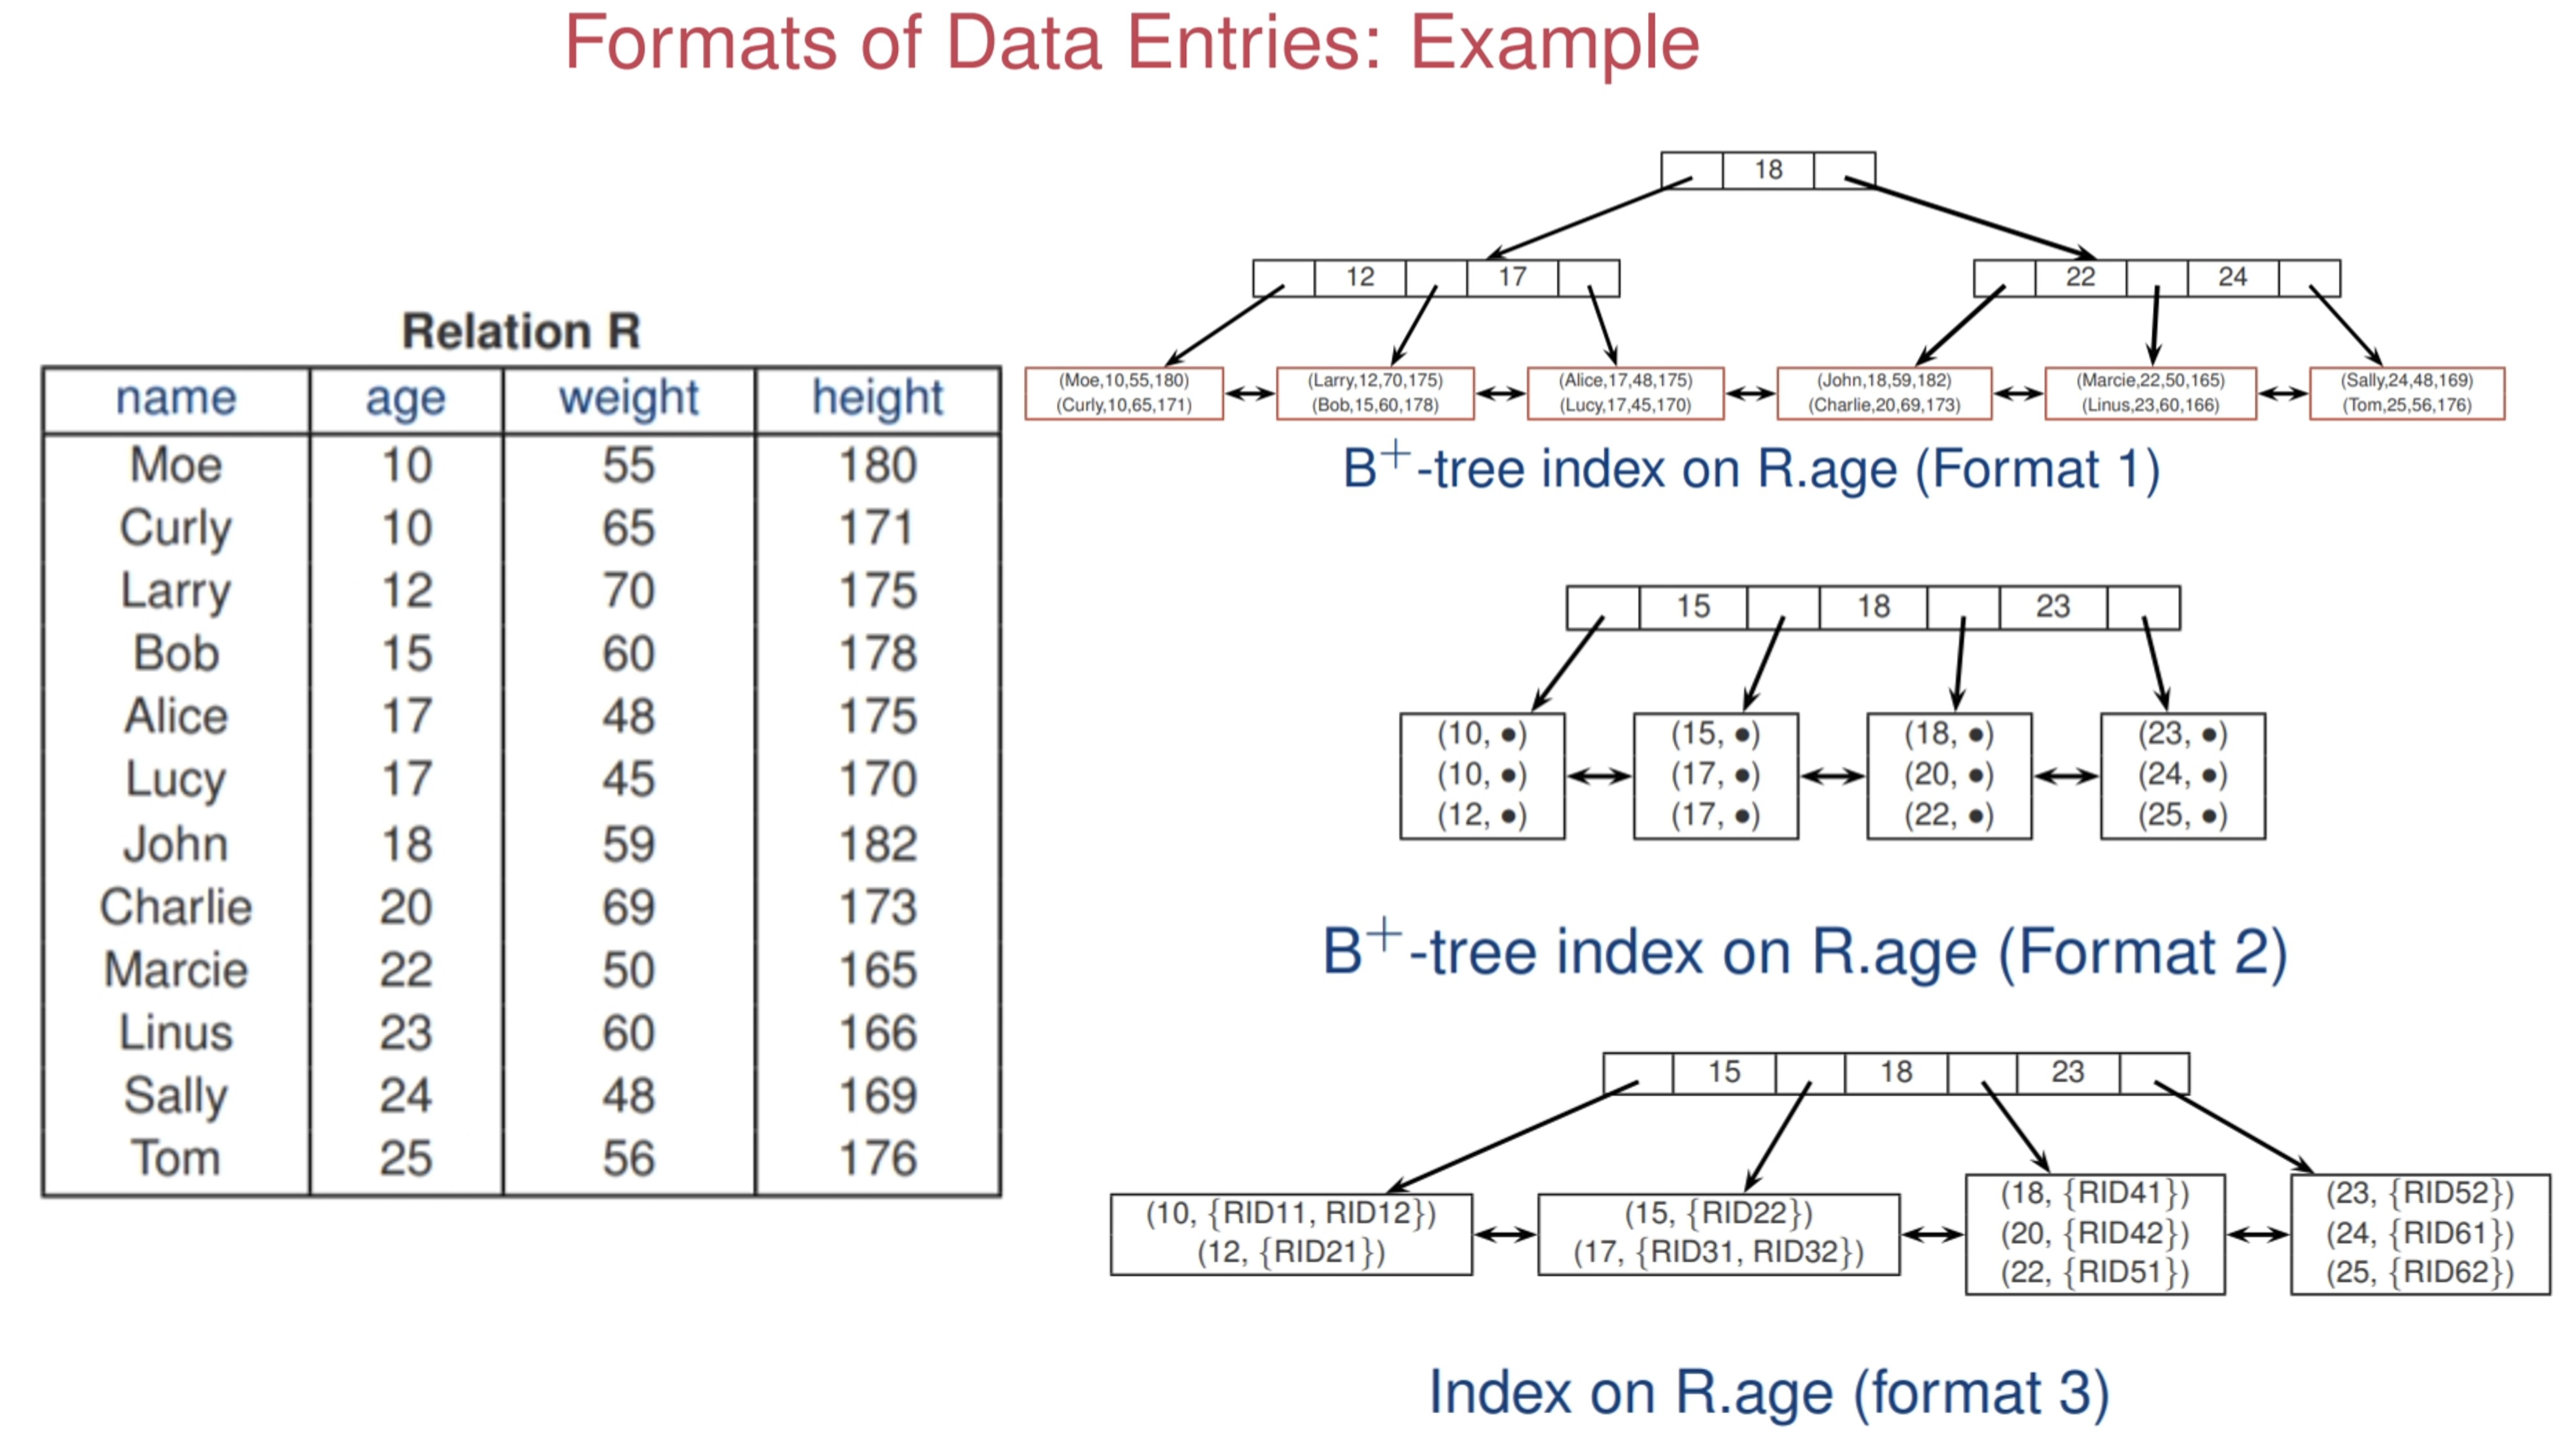
\includegraphics[width = 0.9\linewidth]{dataFormat}}

\subsubsection{$B^+$-tree Search Algorithms }
\begin{itemize}
\item Search algorithm finds the leaf node a given data entry belongs to.
\item We assume no duplicates, no data entries same key value. Note in practice, duplicates arise whenever search key does not contain candidate key, must be dealt with.
\end{itemize}
\centerline{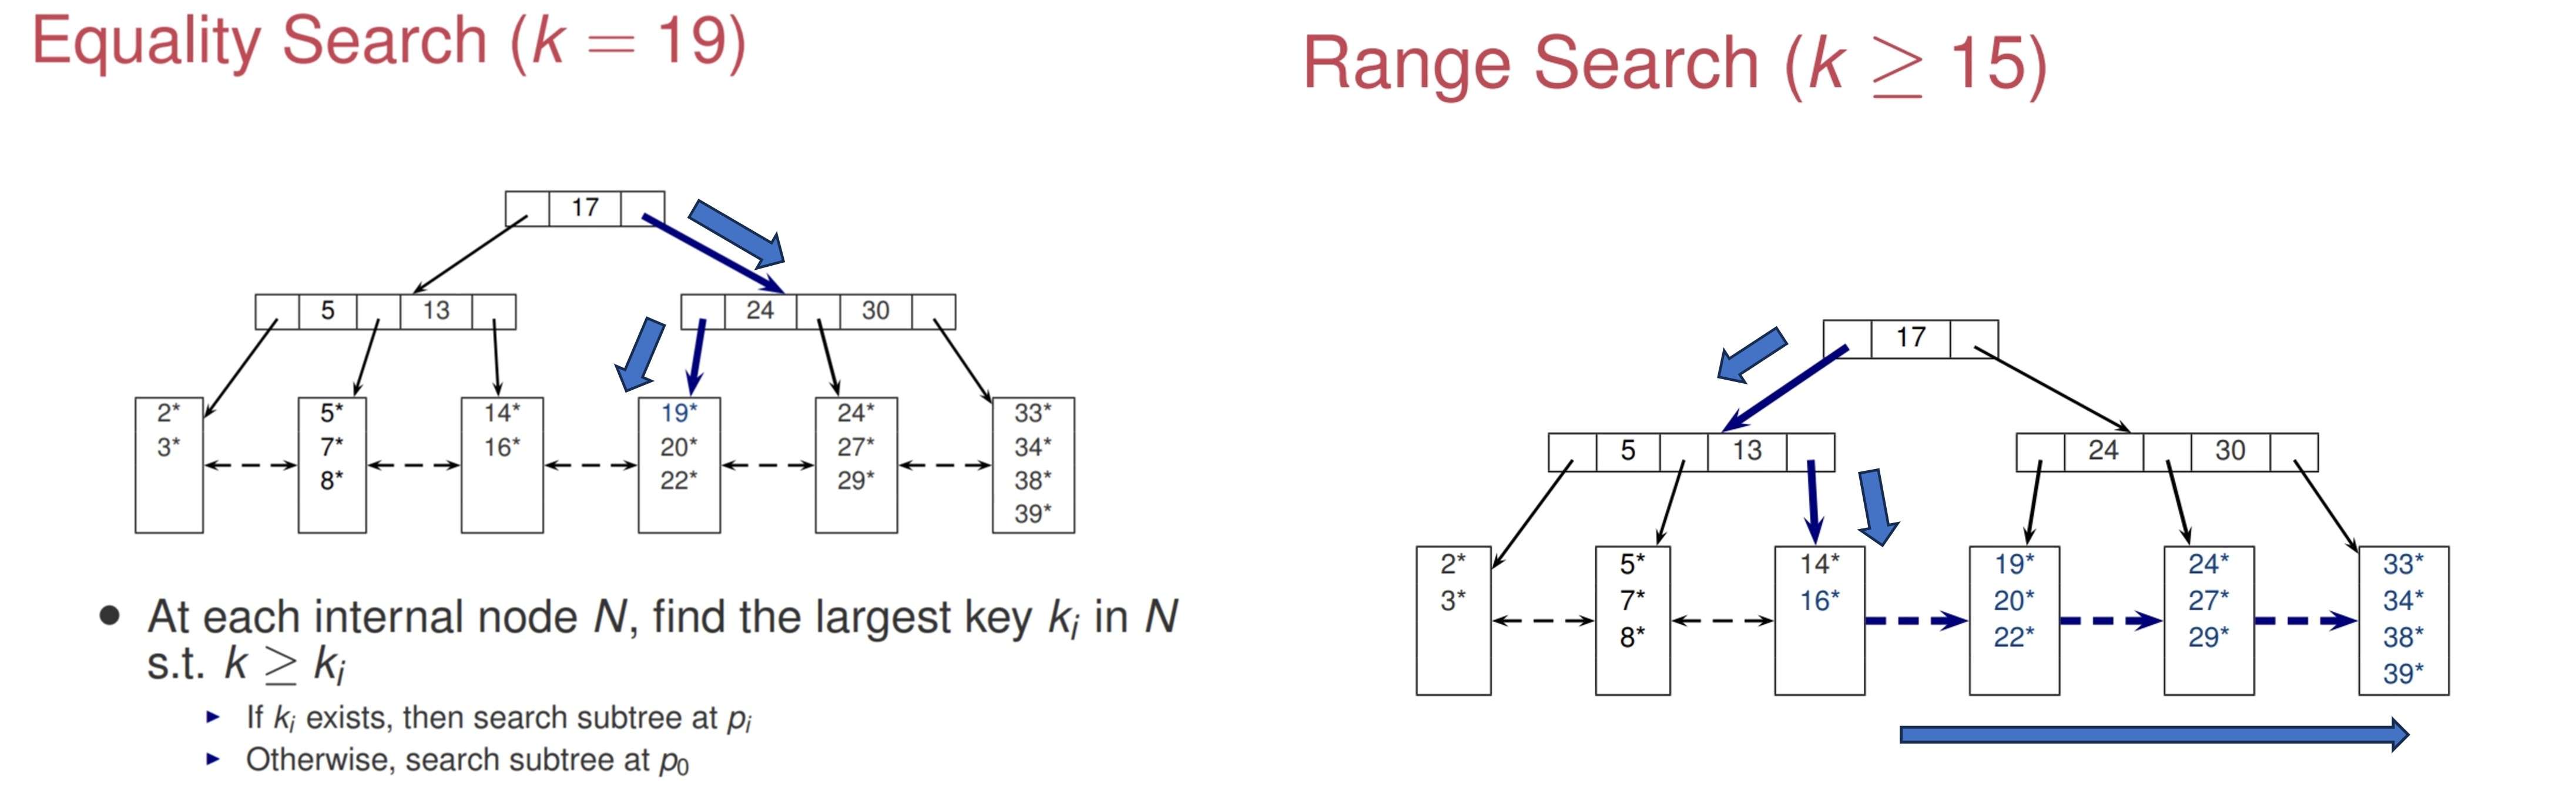
\includegraphics[width = 1\linewidth]{Bsearch}}

\columnbreak

\subsection{$B^+$-Tree Insertion}
\begin{itemize}
\item \textbf{Algorithm for insertion} takes an entry, finds the leaf node where it belongs, and inserts it there.
\item Occasionally, a \textbf{node is full and must be split}. (More than $2d$ entries) When node is split, entry pointing to the node created by the split must be inserted into the parent. 
\item If the (old) root is split, a new root node is created and height of tree increases by 1. 
\end{itemize}


\subsubsection{Splitting of overflowed node}
\begin{itemize}
\item Split overflowed leaf node by distributing $d + 1$ entries to new leaf node.
\item Create a new entry index using smallest key in leaf node.
\item Insert new index entry into parent node of overflowed node.
\end{itemize}
\centerline{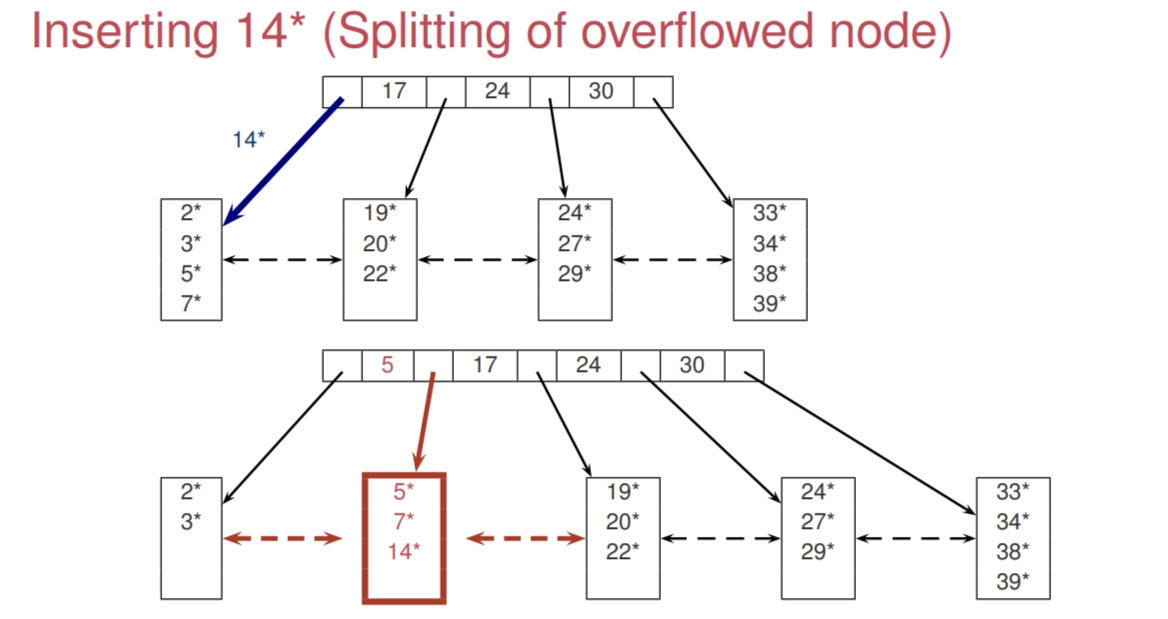
\includegraphics[width = 0.7\linewidth]{Binsertion}}
\begin{itemize}
\item Sometimes, \textbf{node split is propagated upwards} to ancestor internal nodes.
\item When splitting an \textbf{internal node}, the middle key is pushed to parent node.
\end{itemize}
\centerline{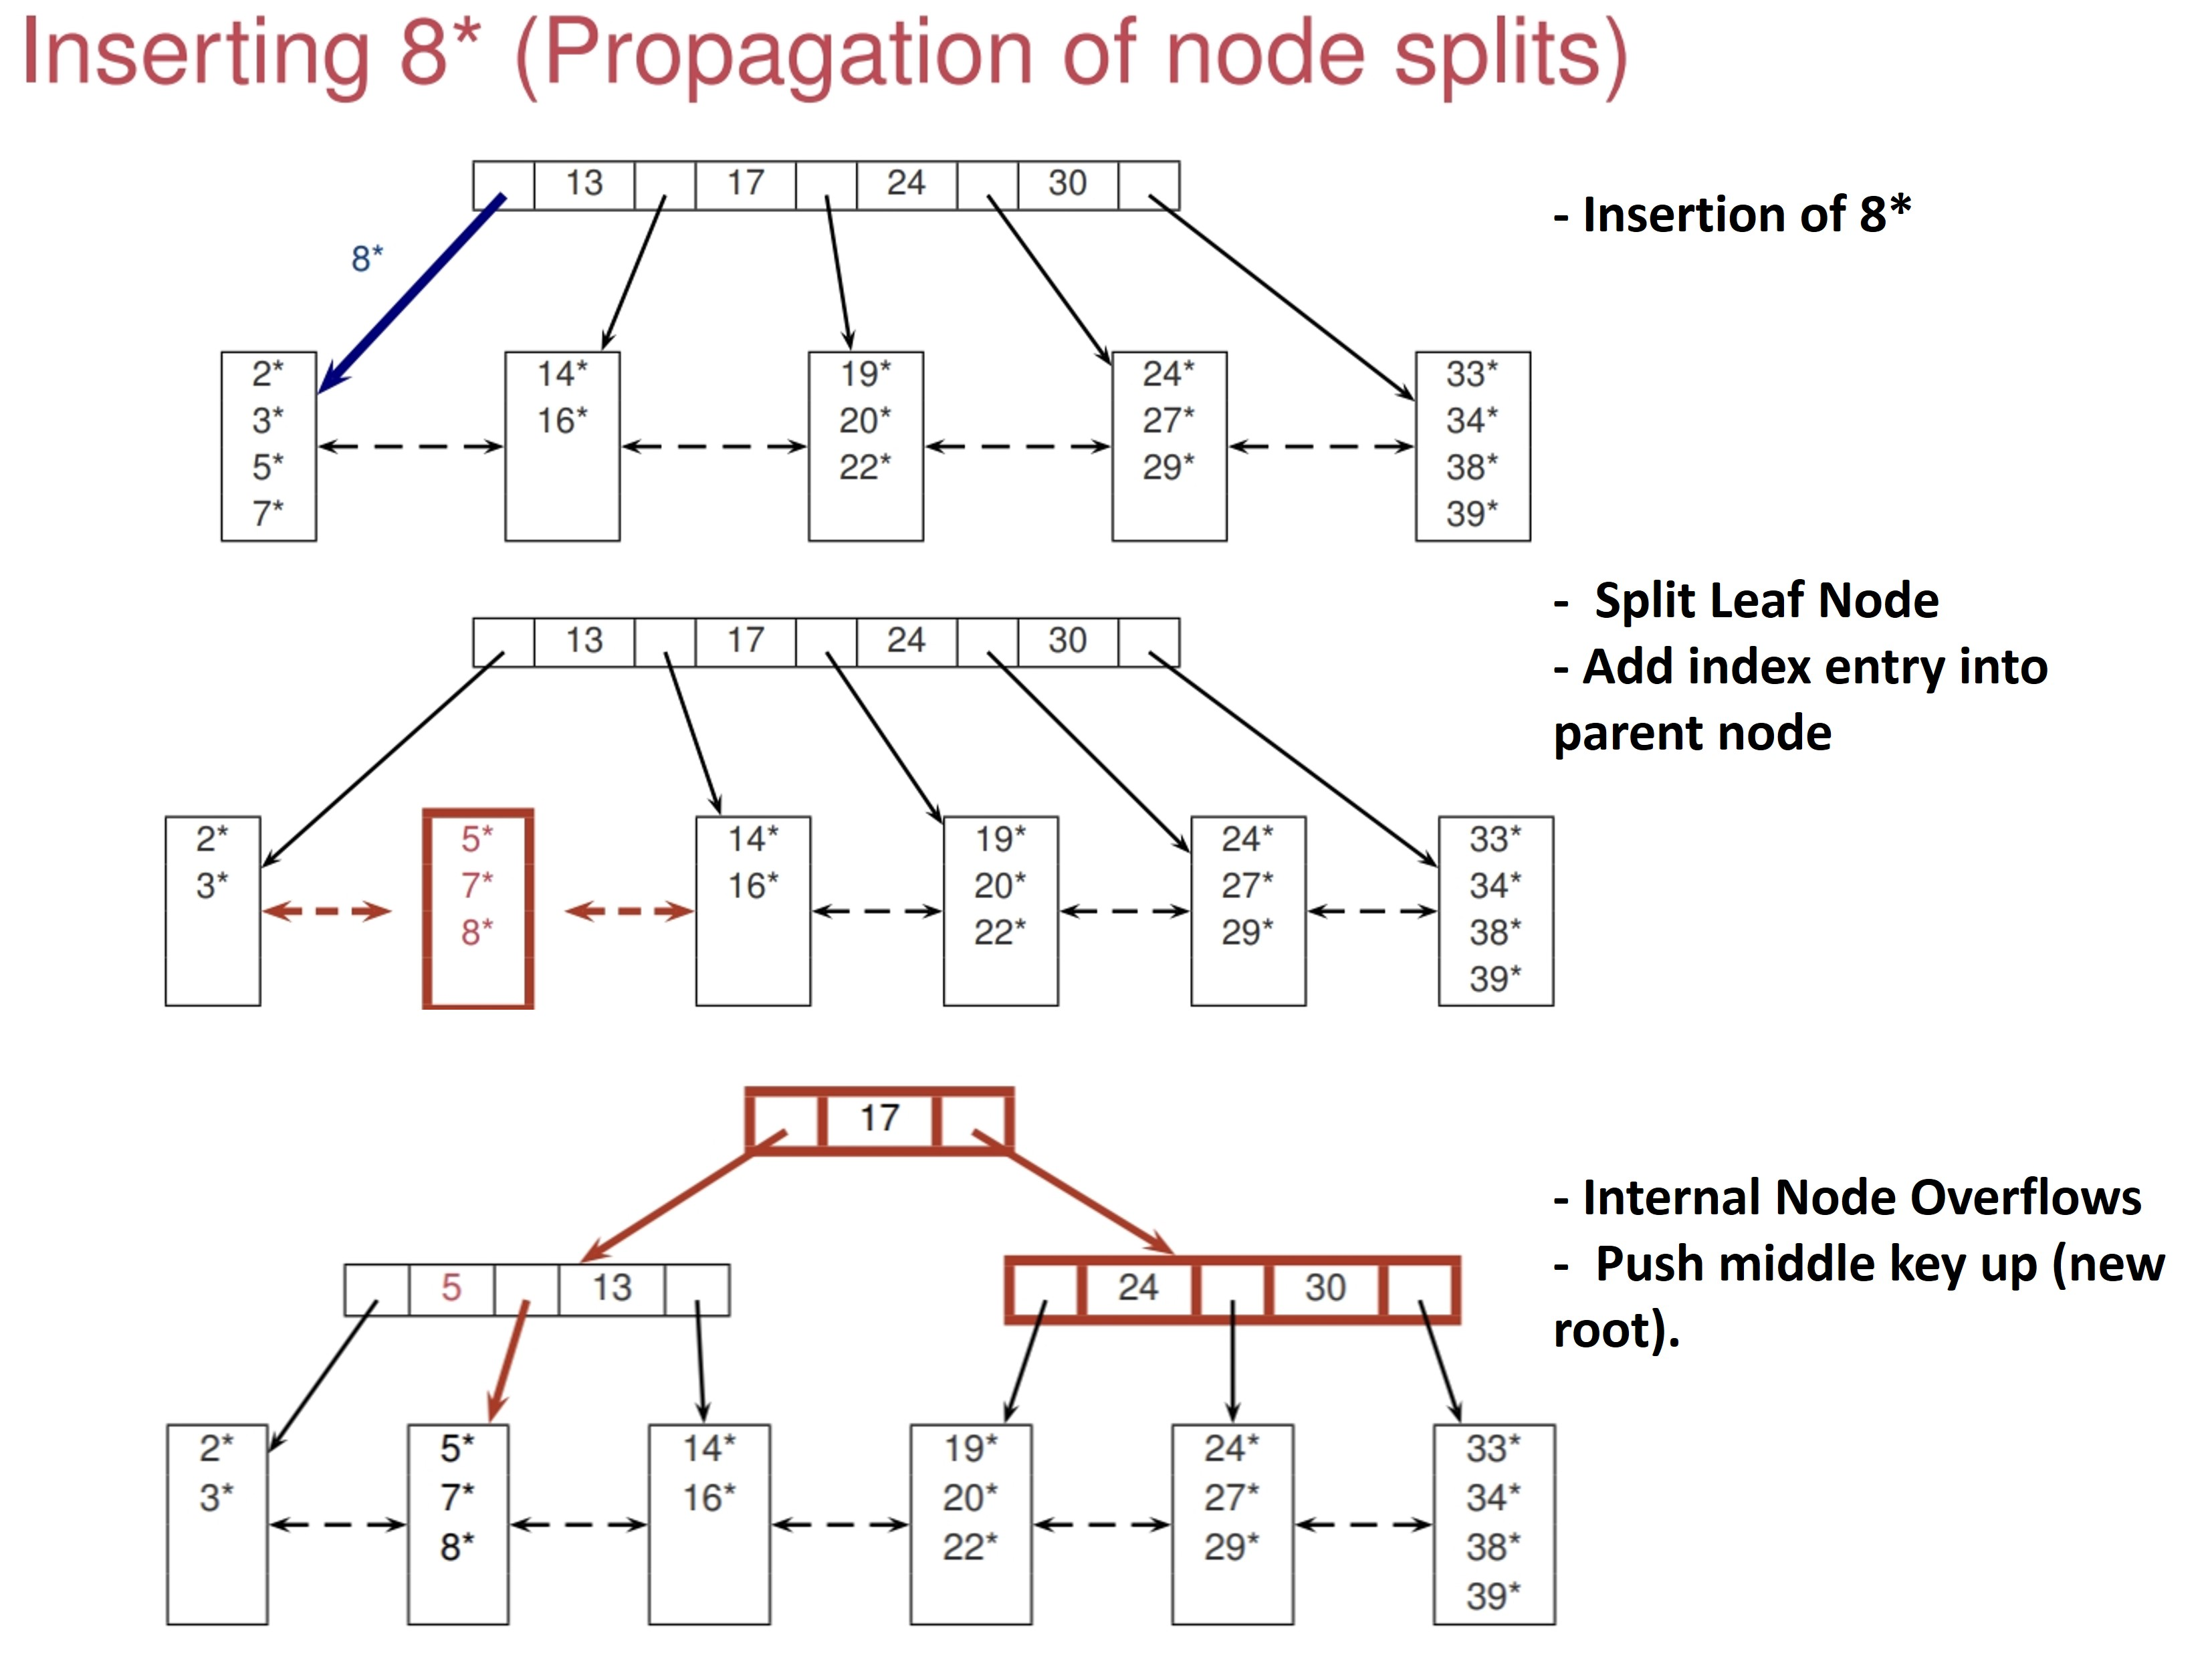
\includegraphics[width = 0.95\linewidth]{Binsertion2}}
\centerline{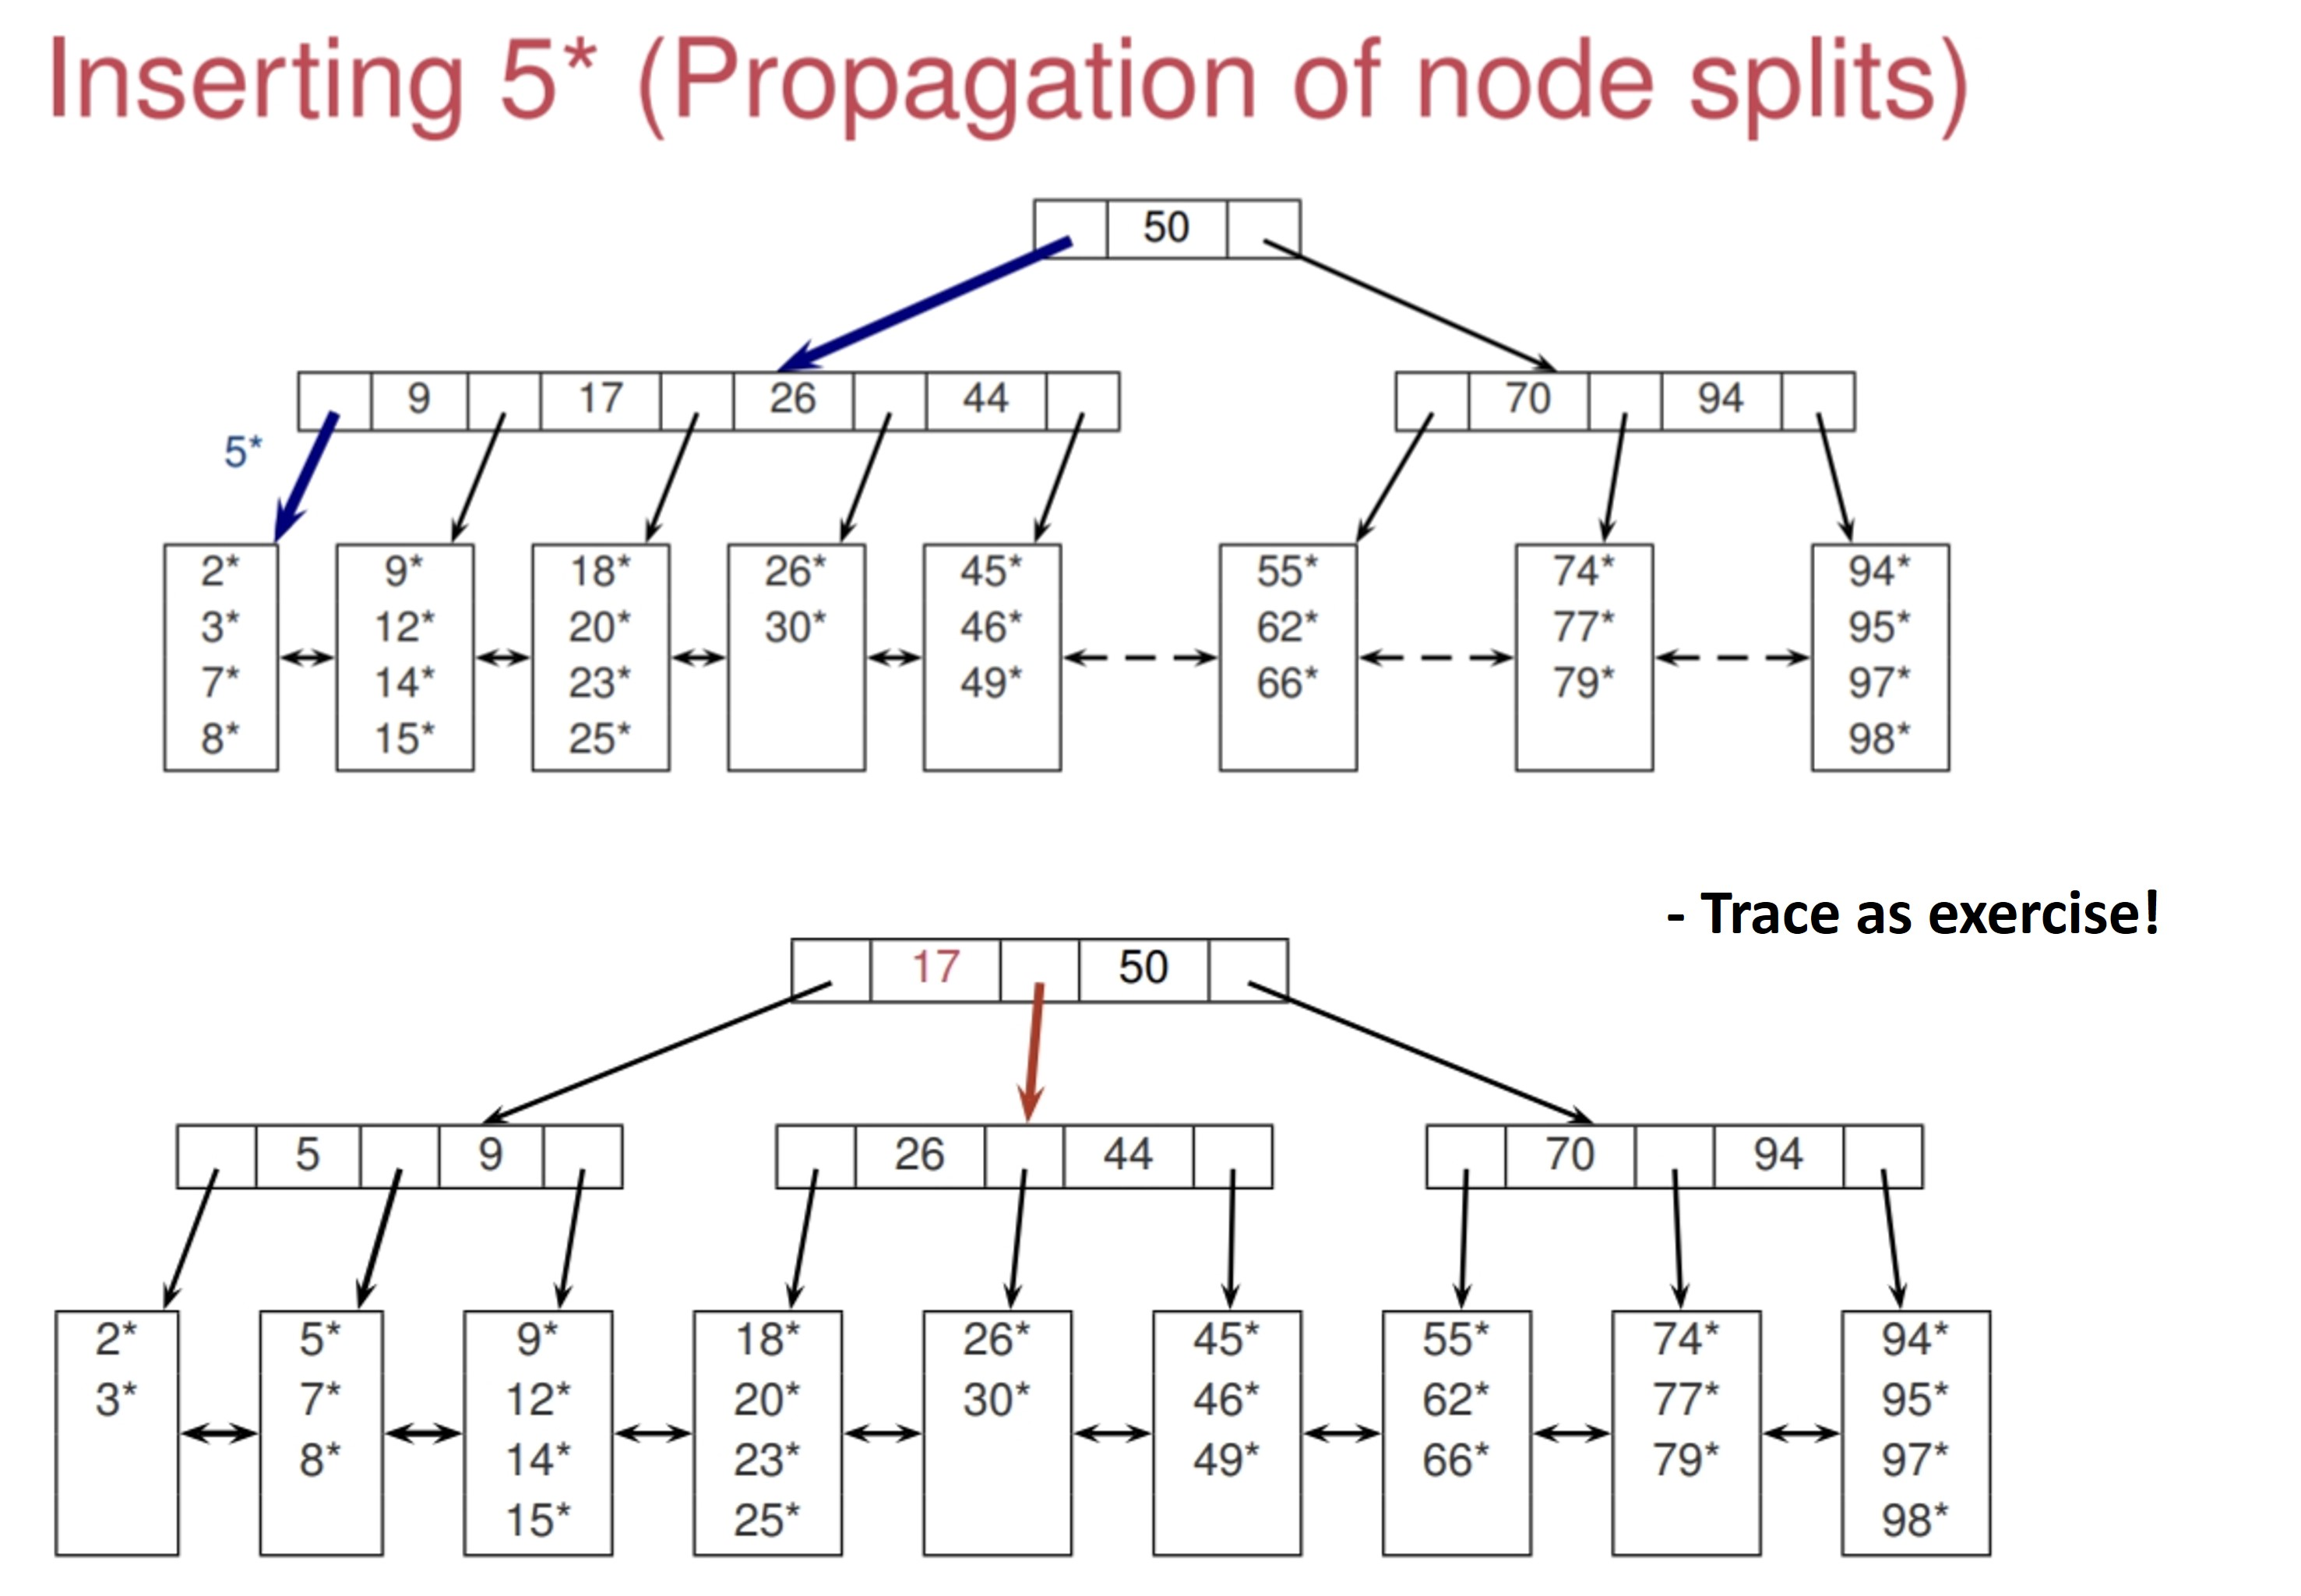
\includegraphics[width = 0.8\linewidth]{Binsertion3}}

\subsubsection{Redistributing of data entries in Overflow}
\begin{itemize}
\item A node split can sometimes be avoided by distributing entries from overflowed node to a non-full adjacent sibling node.
\end{itemize}
\centerline{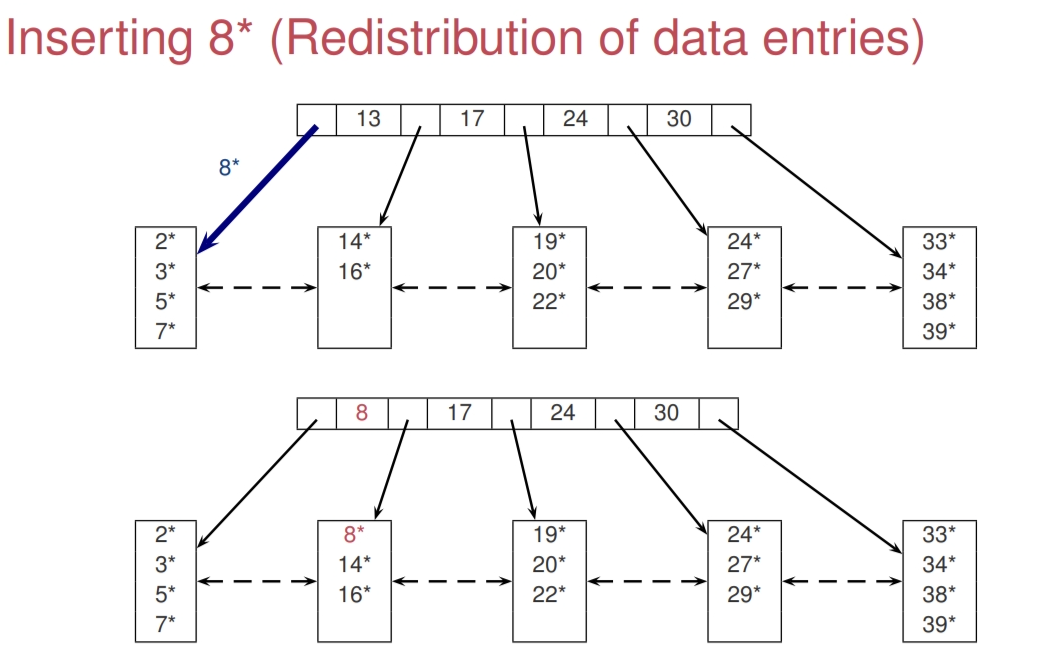
\includegraphics[width = 0.8\linewidth]{Binsertion4}}

\subsection{$B^+$-Tree Deletion}
\begin{itemize}
\item \textbf{Algorithm for deletion} takes an entry, finds leaf node it belongs to, and deletes it.
\item \textbf{Underflowed node}: When node is at minimum occupancy before deletion, and goes below threshold, we must either \textbf{redistribute entries from adjacent sibling}, or \textbf{merge node with sibling} to maintain minimum occupancy.
\item \textbf{Merging}: Underflowed node needs to be merged if each of \textbf{adjacent} sibling nodes has exactly $d$ entries.
\end{itemize}
\centerline{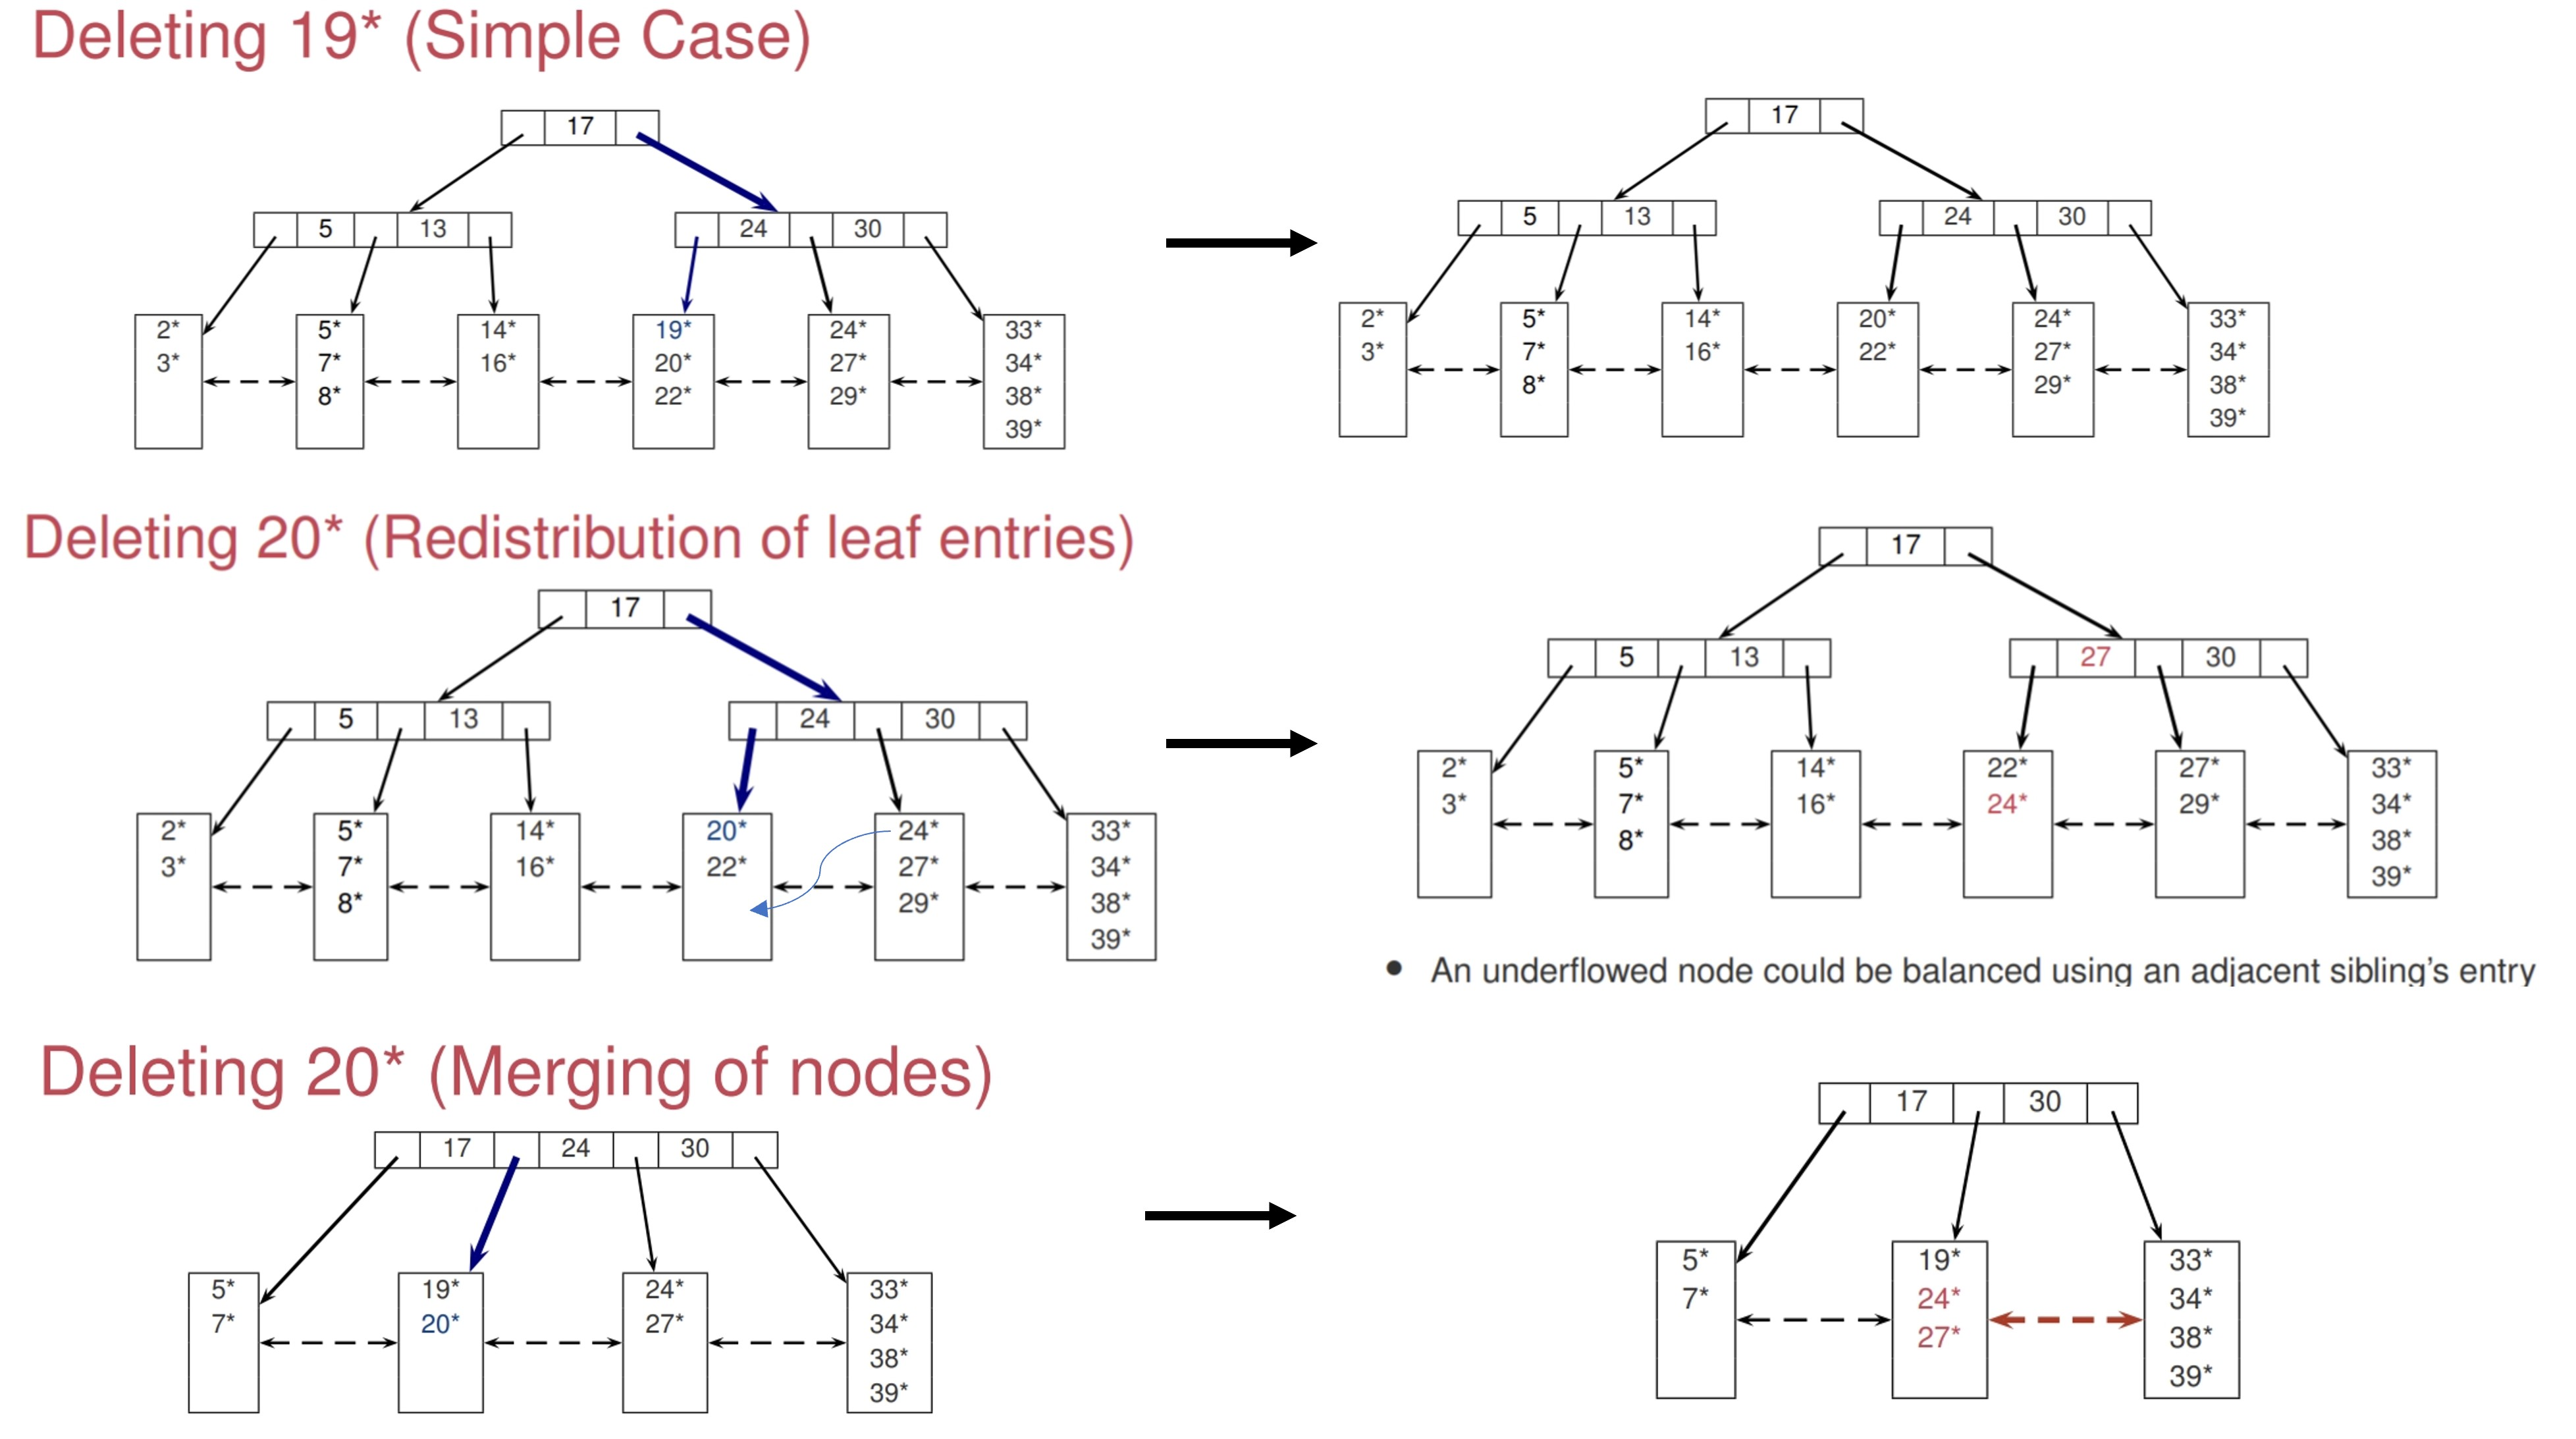
\includegraphics[width = 1\linewidth]{Bdeletion1}}
\begin{itemize}
\item  Node mergers may propagate upwards.
\end{itemize}
\centerline{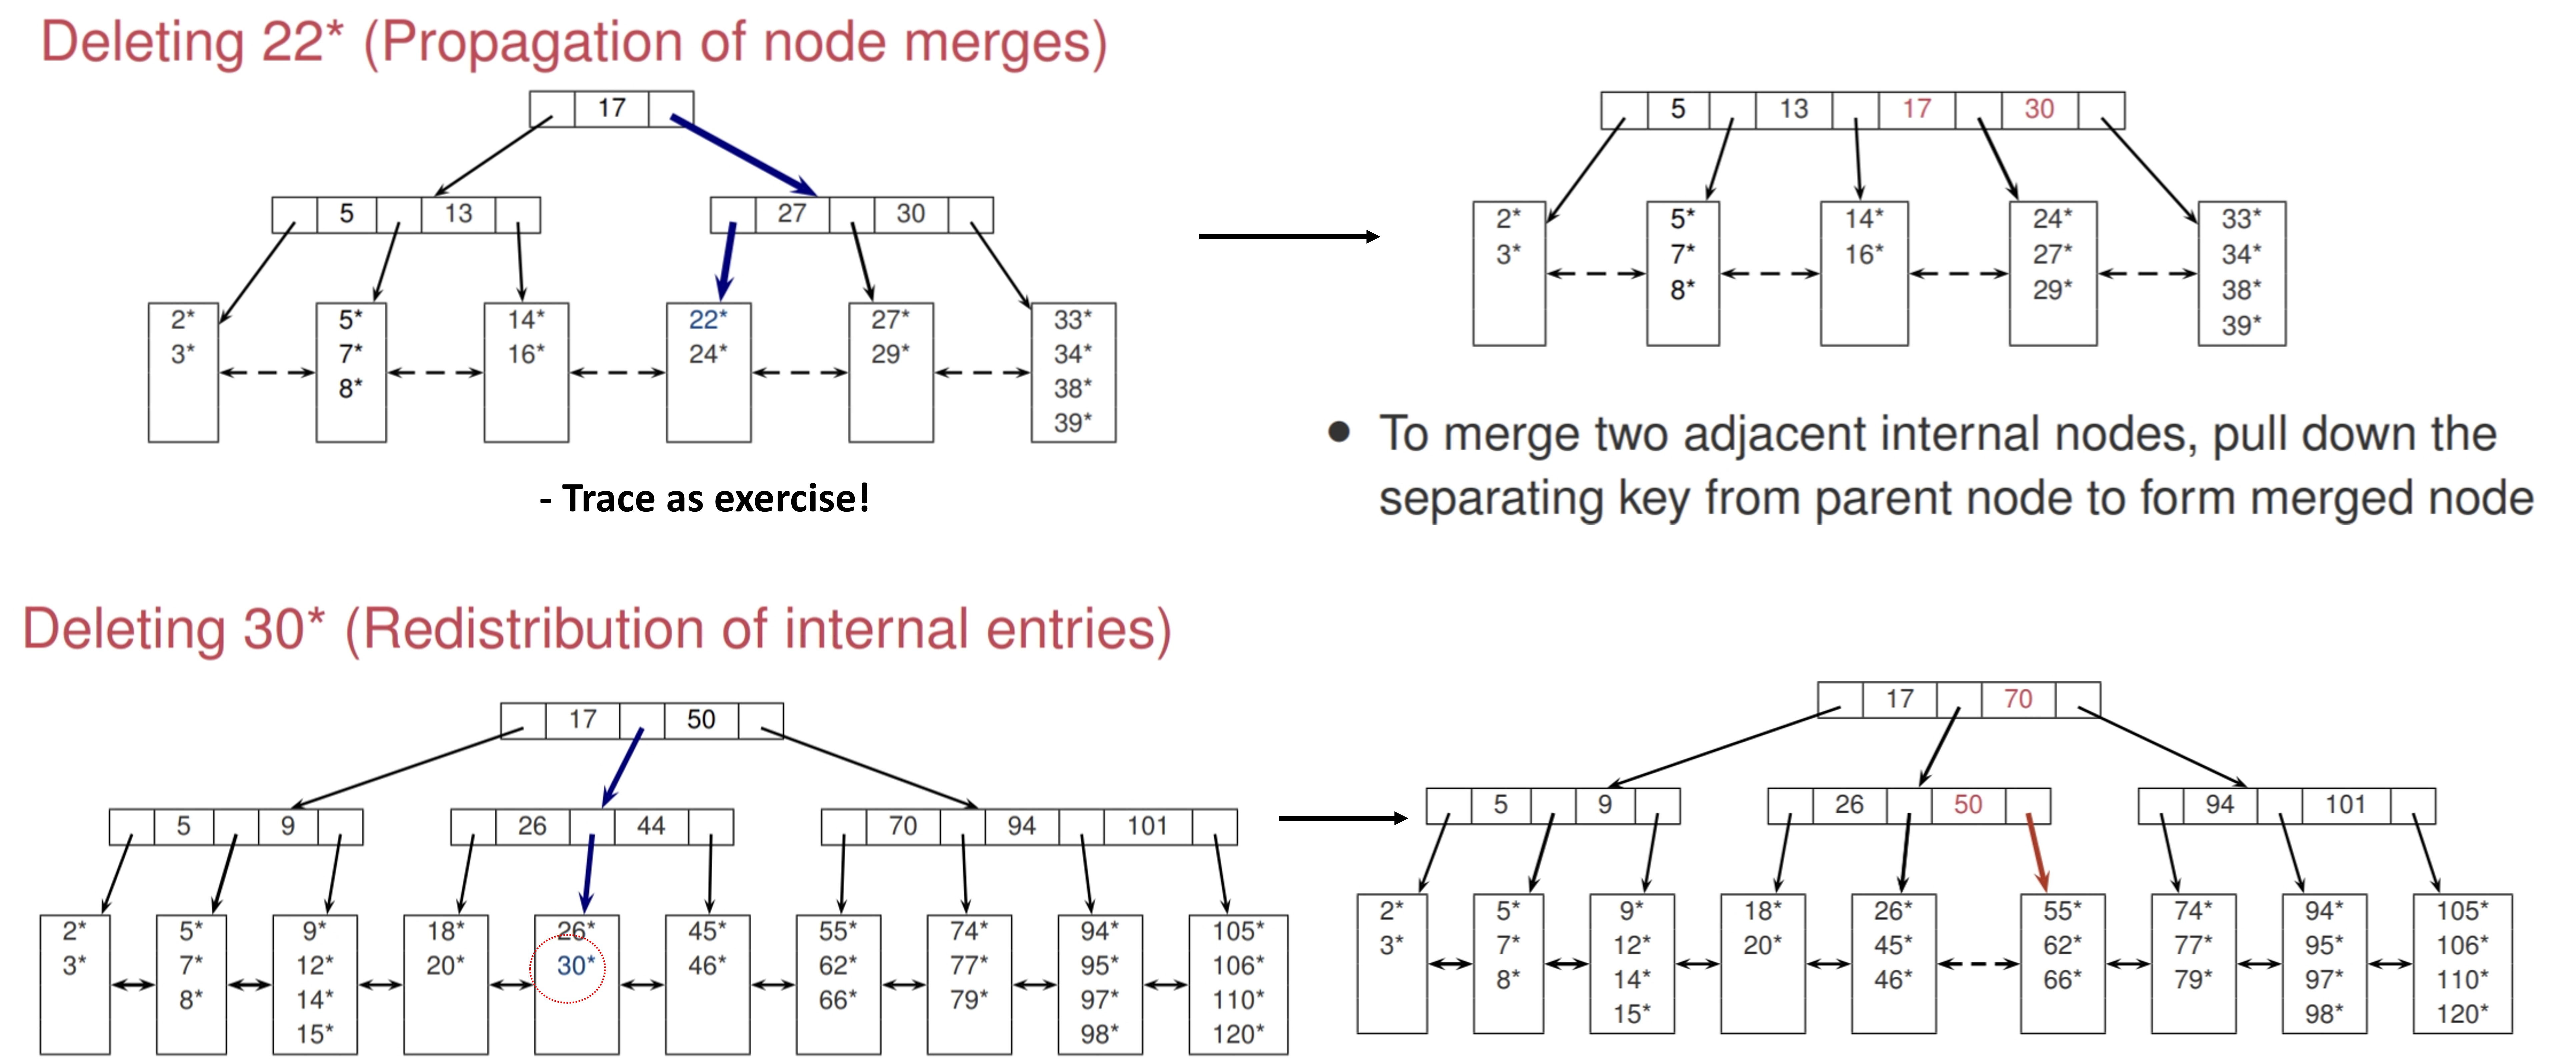
\includegraphics[width = 1\linewidth]{Bdeletion2}}
\begin{itemize}
\item Chances are high that redistribution is possible if node has two siblings, and unlike merging, redistribution is guaranteed to propagate no further than parent node. Also, pages have more space, reducing likelihood of split on subsequent insertions.
\end{itemize}

\columnbreak

\subsection{$B^+$-Tree Bulk Loading}
\begin{itemize}
\item Entries added to a $B^+$ in two ways.
	\begin{enumerate}
	\item Have existing collection of data records with $B^+$ tree index on it. When record added to collection, corresponding entry added to $B^+$ tree. (Insert, Delete individually)
	\item Have collection of data records we want to create new $B^+$ tree index on some key field(s). Start with an empty tree. Inserting one by one expensive due to overhead, systems provide \textbf{bulk loading} utility.
	\end{enumerate}
\item \textbf{Bulk Loading}: 
	\begin{enumerate}
	\item Sort data entries $k*$ to be inserted into $B^+$ tree according to search key $k$. (Here, $d$ = 1).
	\item Allocate empty page to serve as root. Insert a pointer to first page of (sorted entries into it).
	\centerline{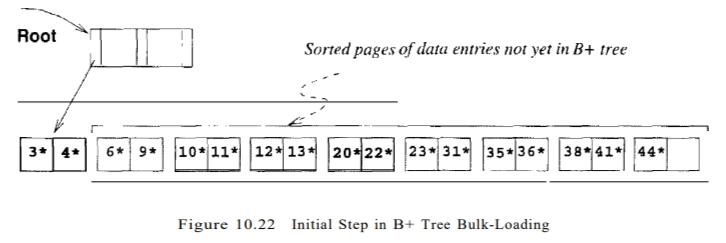
\includegraphics[width = 0.8\linewidth]{bulkloading1}}
	\item Add one entry to root page for each page of sorted data entries. Proceed until root page is full. Here, we must split root and create a new root page.
	\centerline{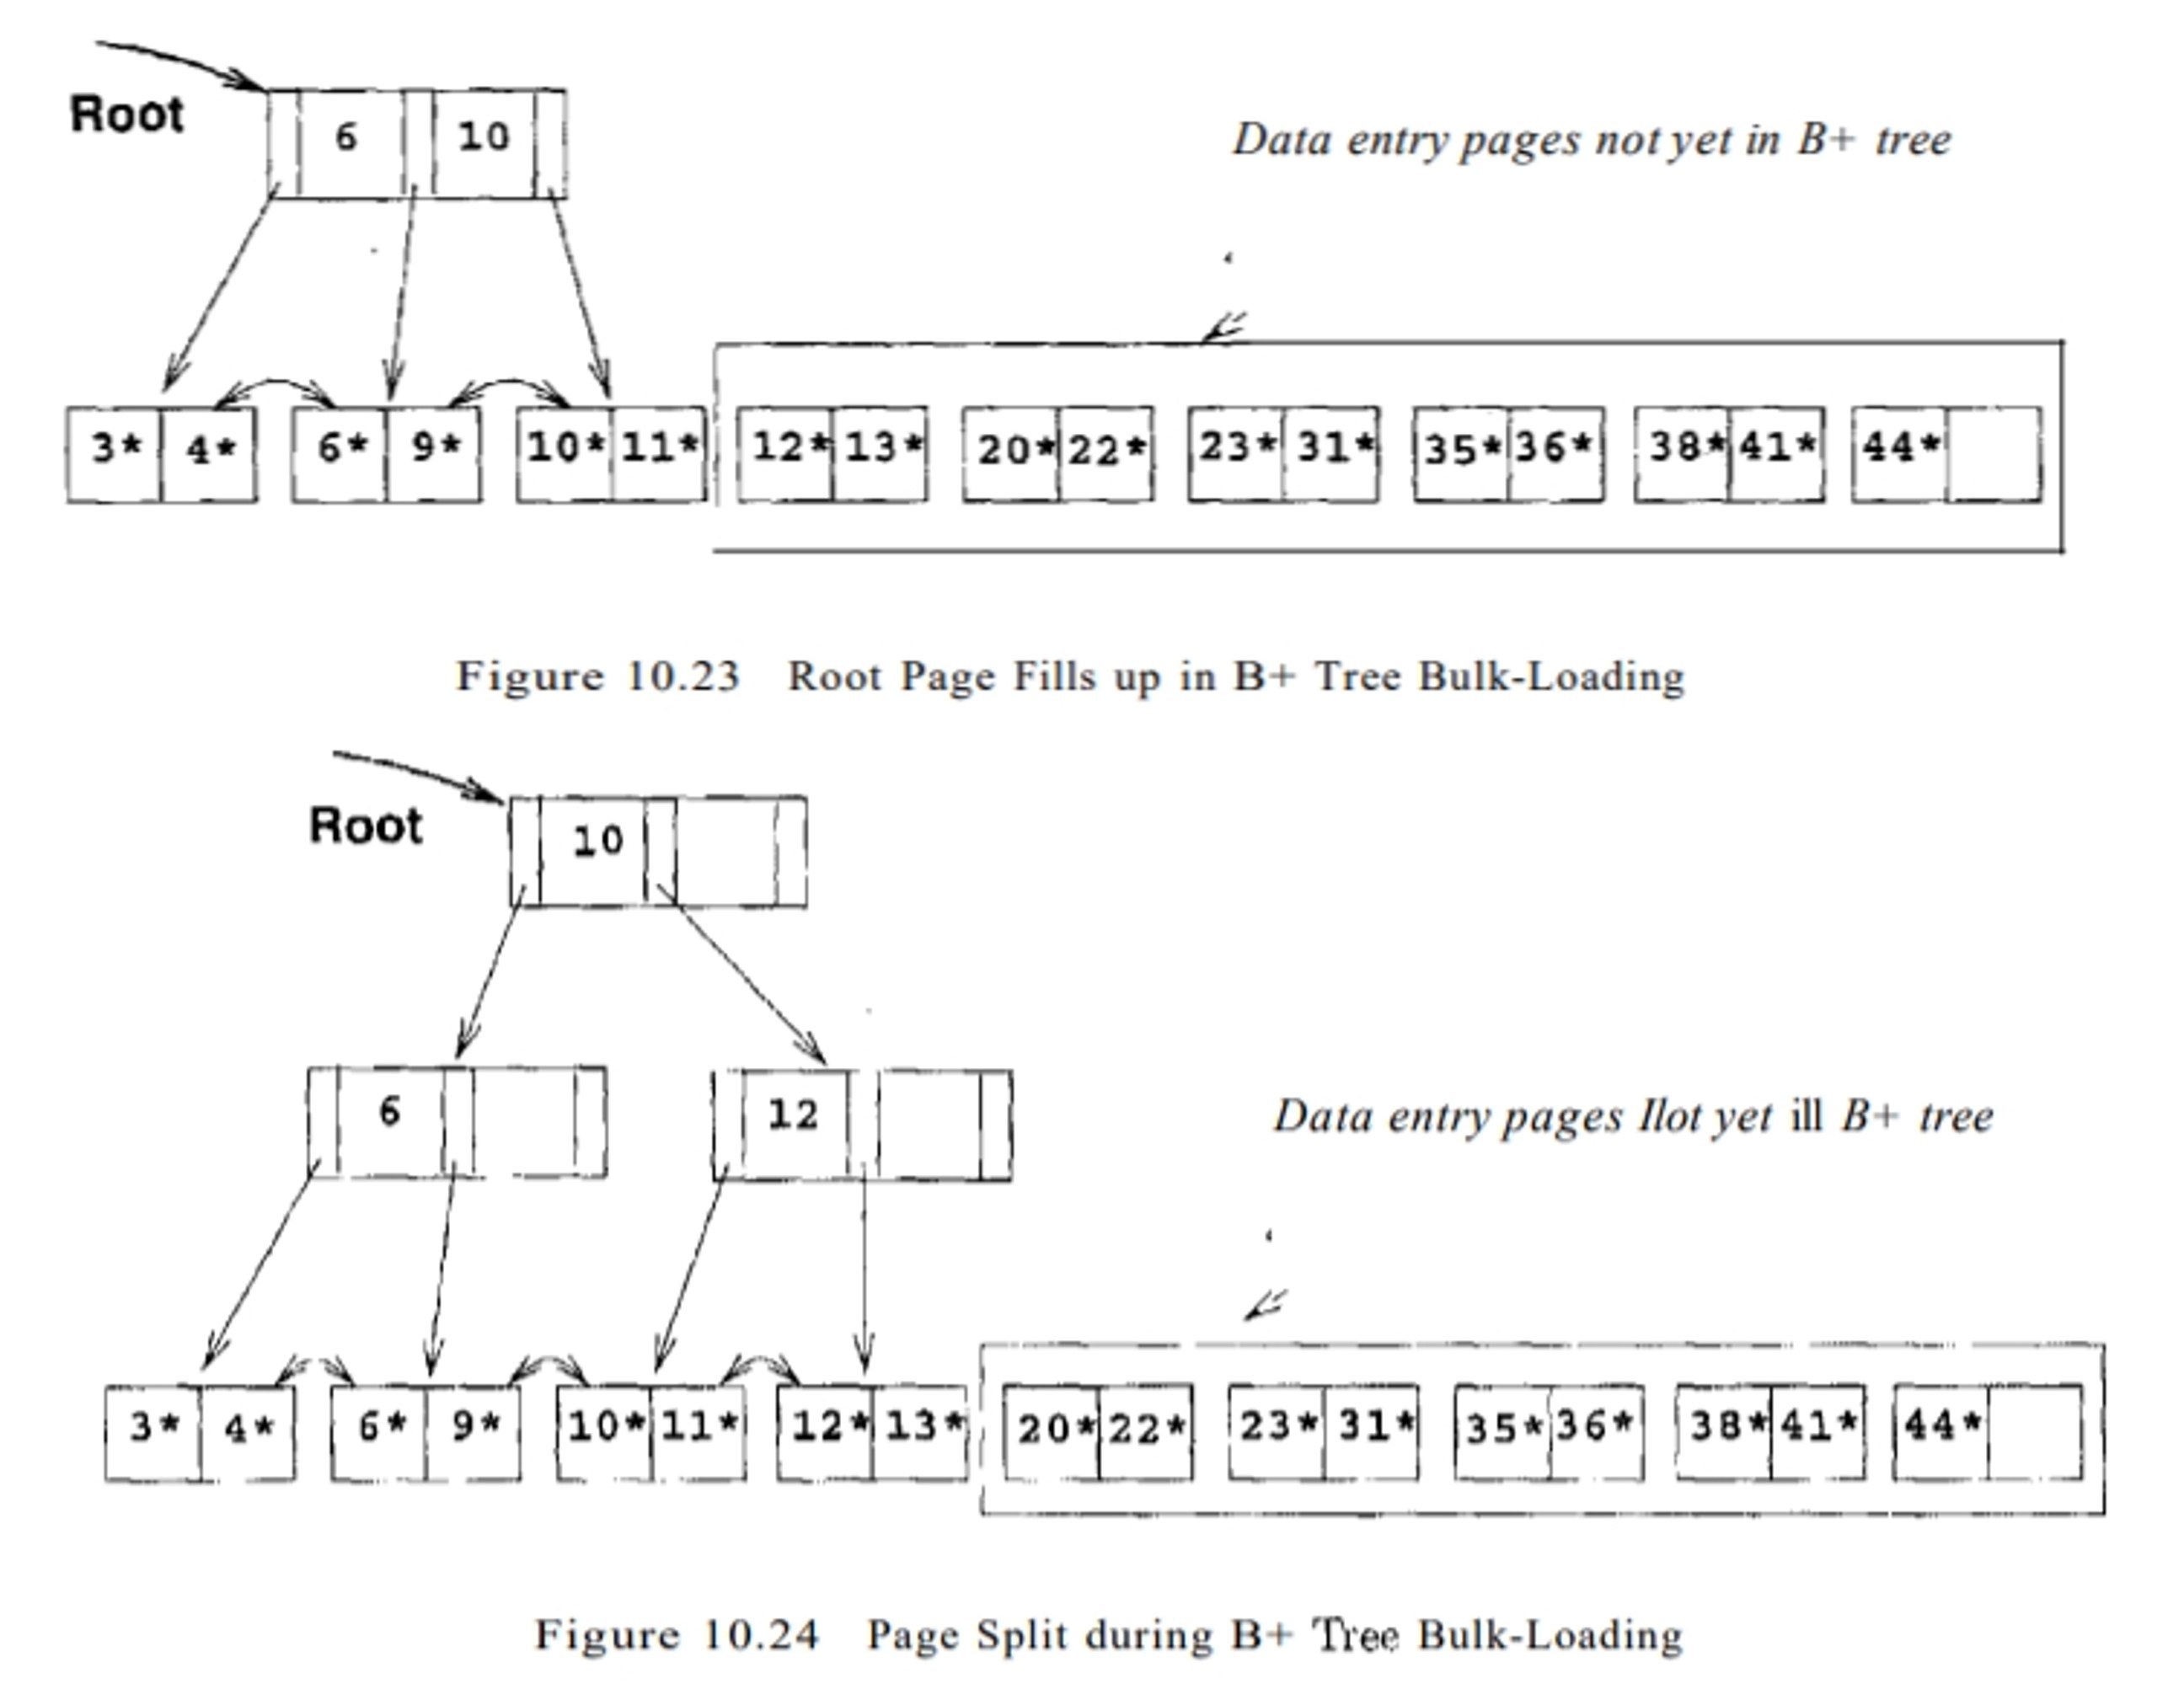
\includegraphics[width = 0.8\linewidth]{bulkloading2}}
	\item To continue, entries for leaf pages \textbf{always inserted into right-most index page just above the leaf level}. When right-most page above leaf level fills up, it is split.
	\centerline{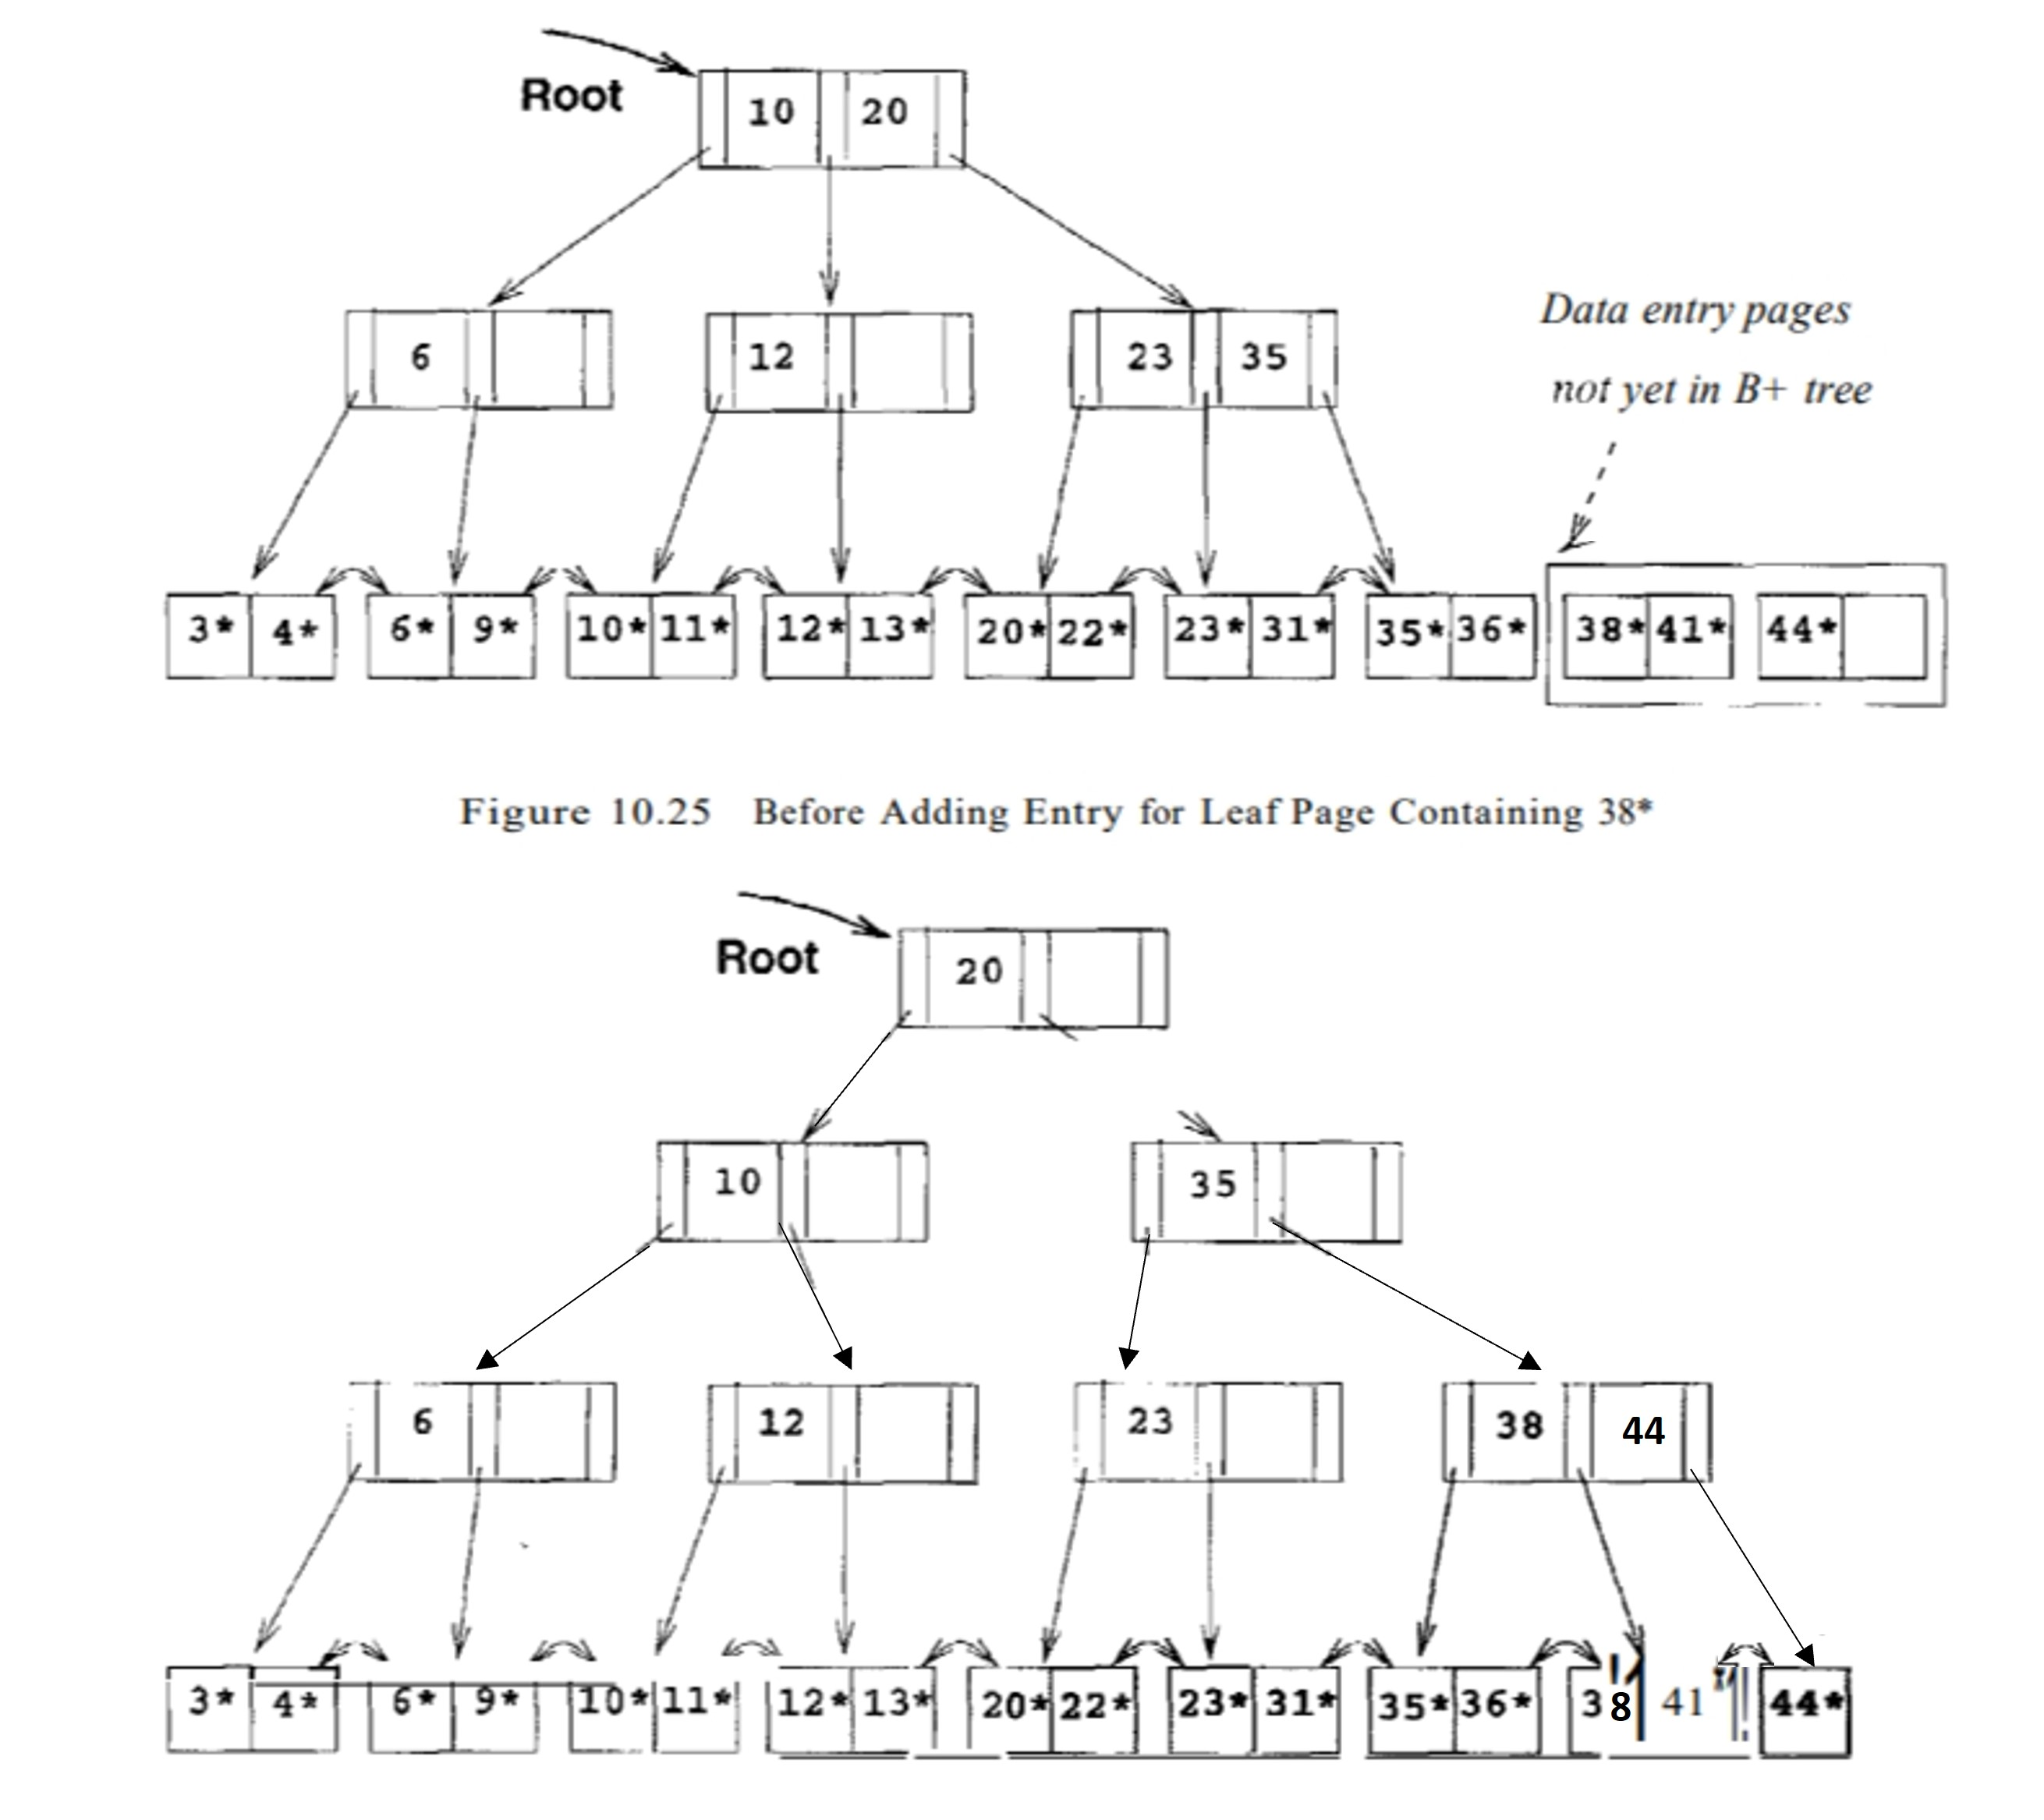
\includegraphics[width = 0.7\linewidth]{bulkloading3}}
	\end{enumerate}
\end{itemize}

\section{3. Hash-based Indexing}
\begin{itemize}
\item Used for \textbf{equality queries}, not for range queries.
\item \textbf{Hashing techniques}: \textbf{Static hashing, dynamic hashing} (linear hashing, extendible hashing, etc).
\end{itemize}

\subsection{Static Hashing}
\begin{itemize}
\item \textbf{Data stored in $N$ buckets}, fixed at creation time. Bucket consists of \textbf{one primary data page \& chain} of zero or more overflow data pages.
\item $v$* represents data entry $e$ with h(e.key) = $v$, not search entry with RID. 
\item \textbf{Problem with static hashing}: As data grows, longer overflow chain, efficiency drops. Need to periodically rehash and increase no. of buckets.
\end{itemize}
\centerline{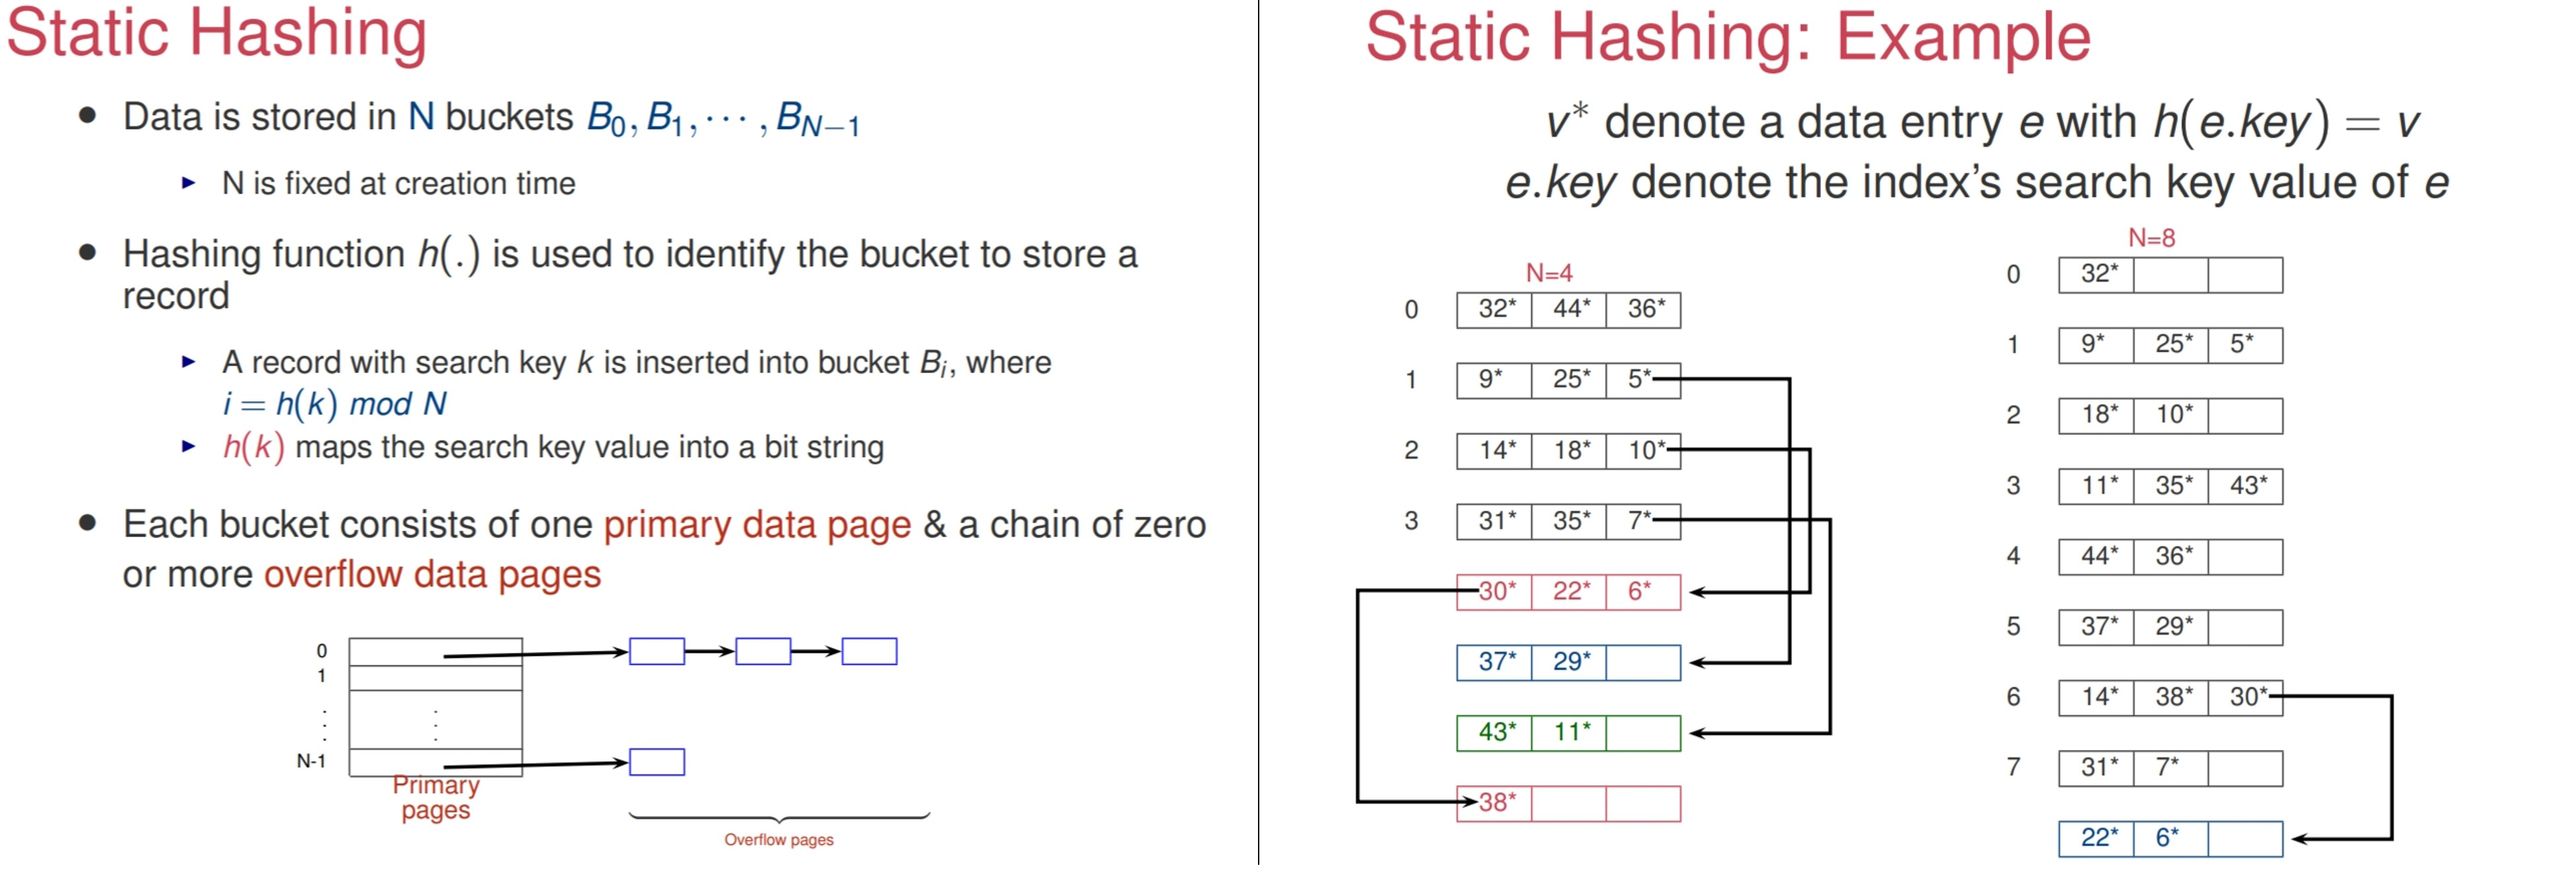
\includegraphics[width = 0.95\linewidth]{staticHashing}}


\subsection{Dynamic Hashing: Linear Hashing}
\begin{itemize}
\item Hash file grows / shrinks linearly, systematic \textbf{splitting of buckets}.
\item Overflow pages needed as overflowed bucket may not be split immediately. 
\item Hashing function changes dynamically and at given instant, \textbf{at most two (successive) hashing functions} used by the scheme during search.
\item Each bucket has primary data page \& chain of zero+ overflow pages.
\item Insert in bucket $B_i$ overflows if all pages in $B_i$ (primary + overflow) full.
\end{itemize}
\centerline{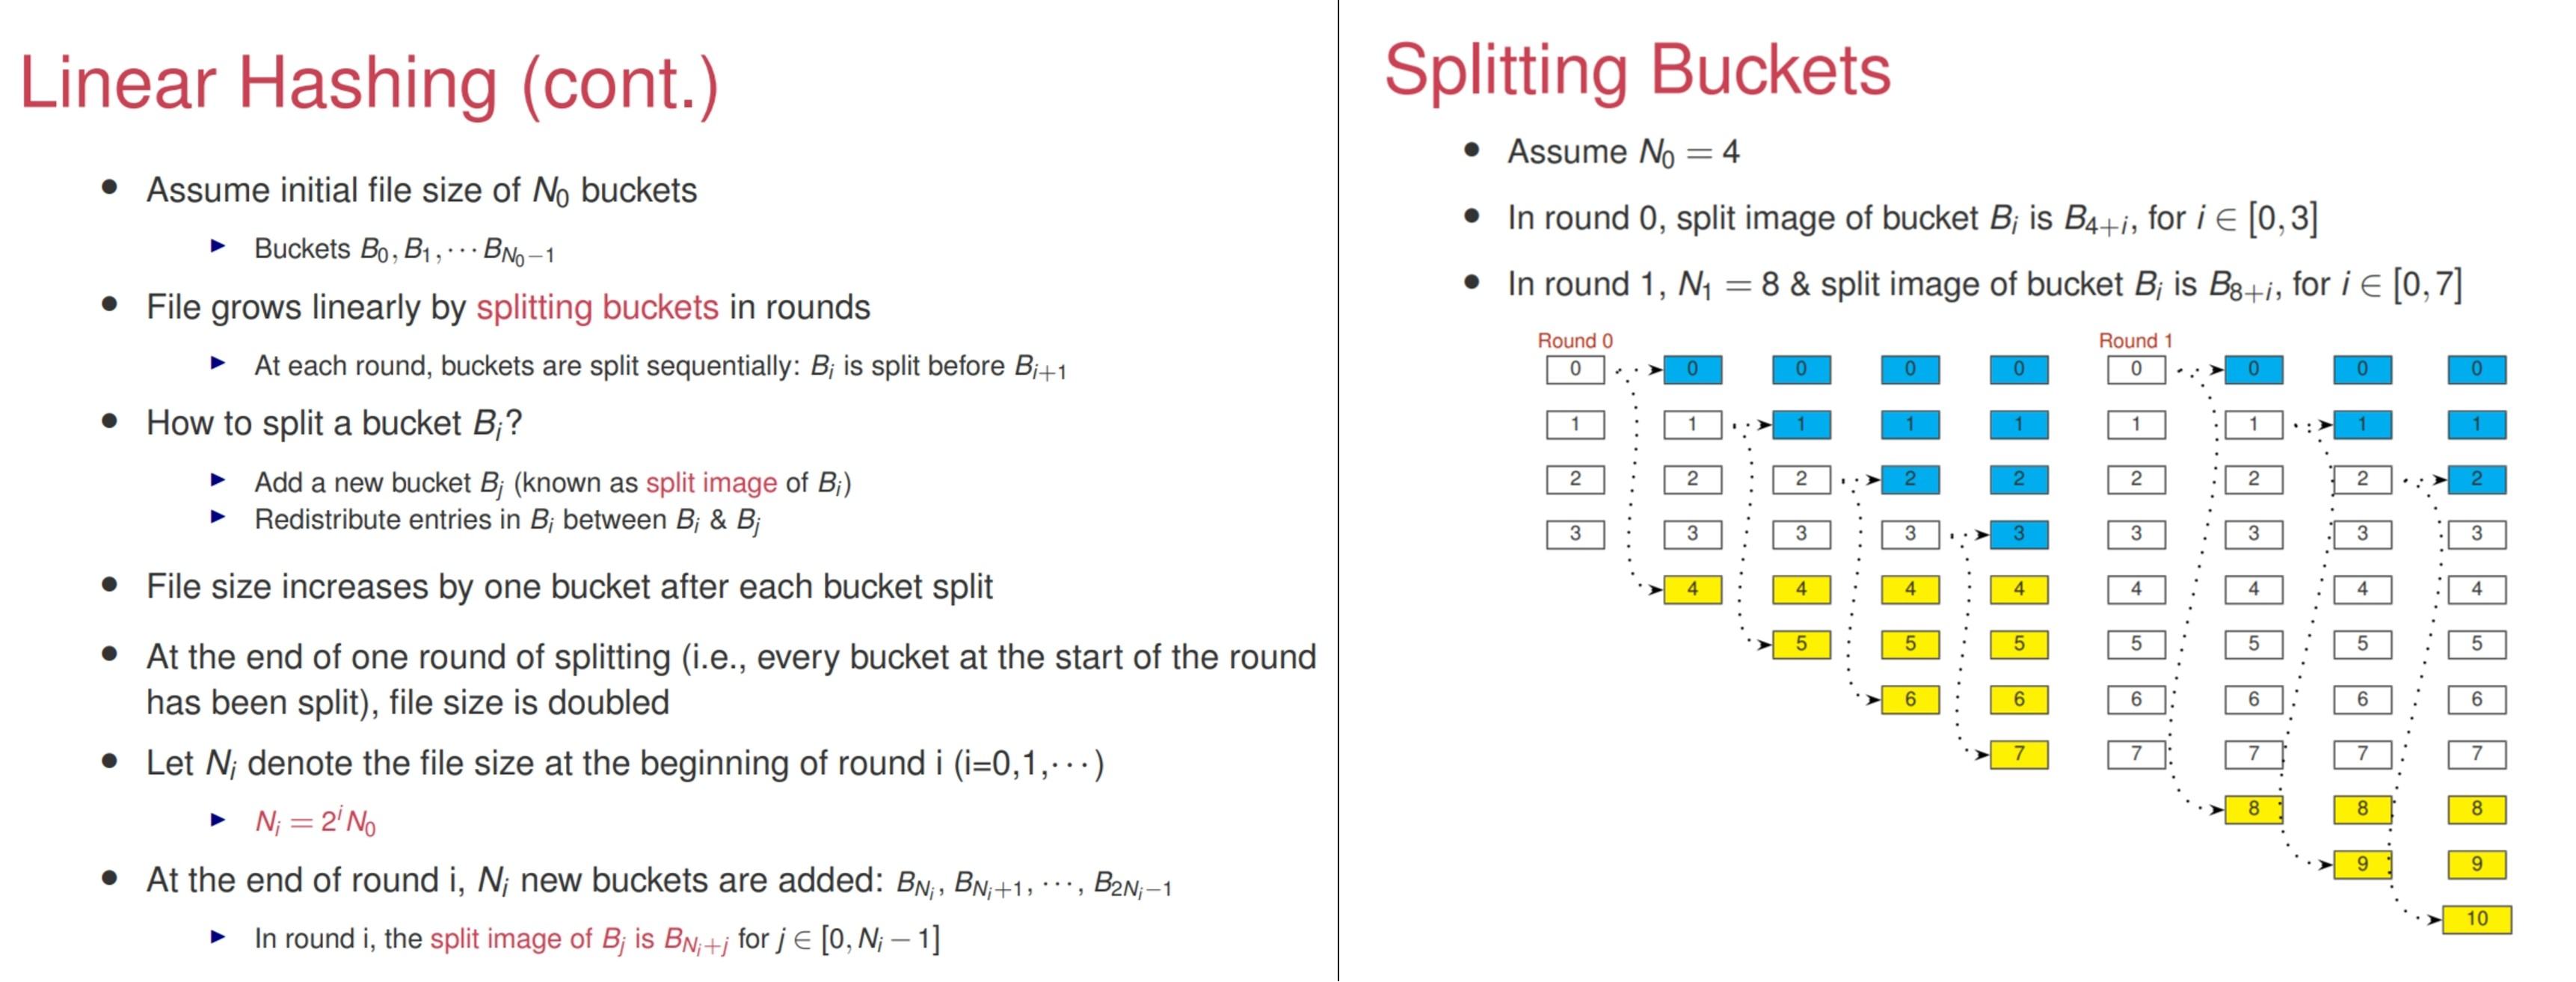
\includegraphics[width = 1\linewidth]{linearHashing}}

\subsubsection{Dynamicity of Linear Hashing}
\centerline{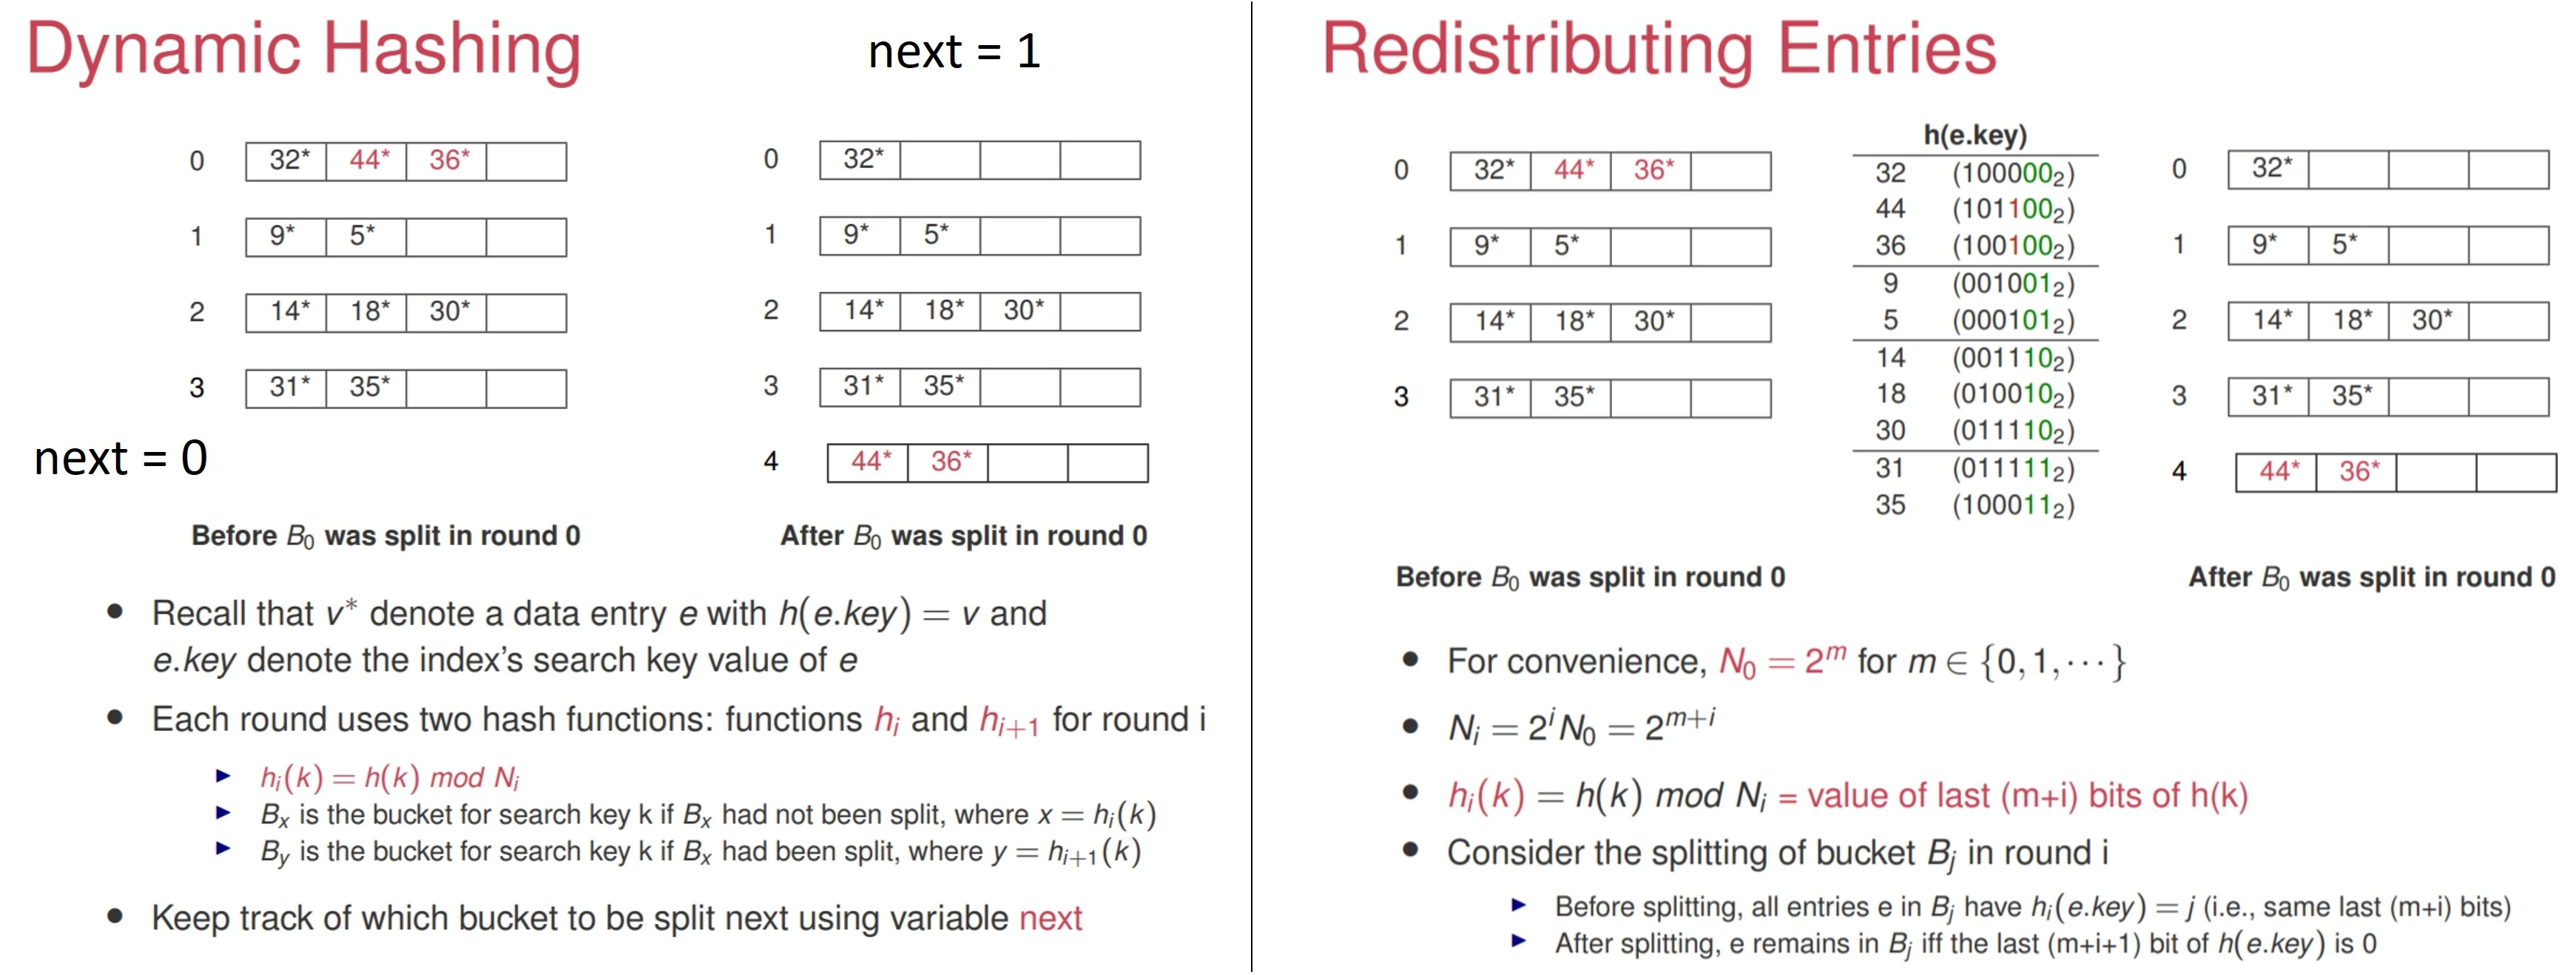
\includegraphics[width = 1\linewidth]{dynamicHashing}}

\subsubsection{Linear (Hashing) Splitting of Buckets (Insertion)}
\begin{itemize}
\item Number in buckets represent the rightmost bit values.
\item \textbf{Split Criteria}: variable, could be when some bucket overflow, space utilization of file above some threshold etc.
\item \textbf{Level}: We use level to denote splitting round number (use with \textbf{next}).
\end{itemize}
\centerline{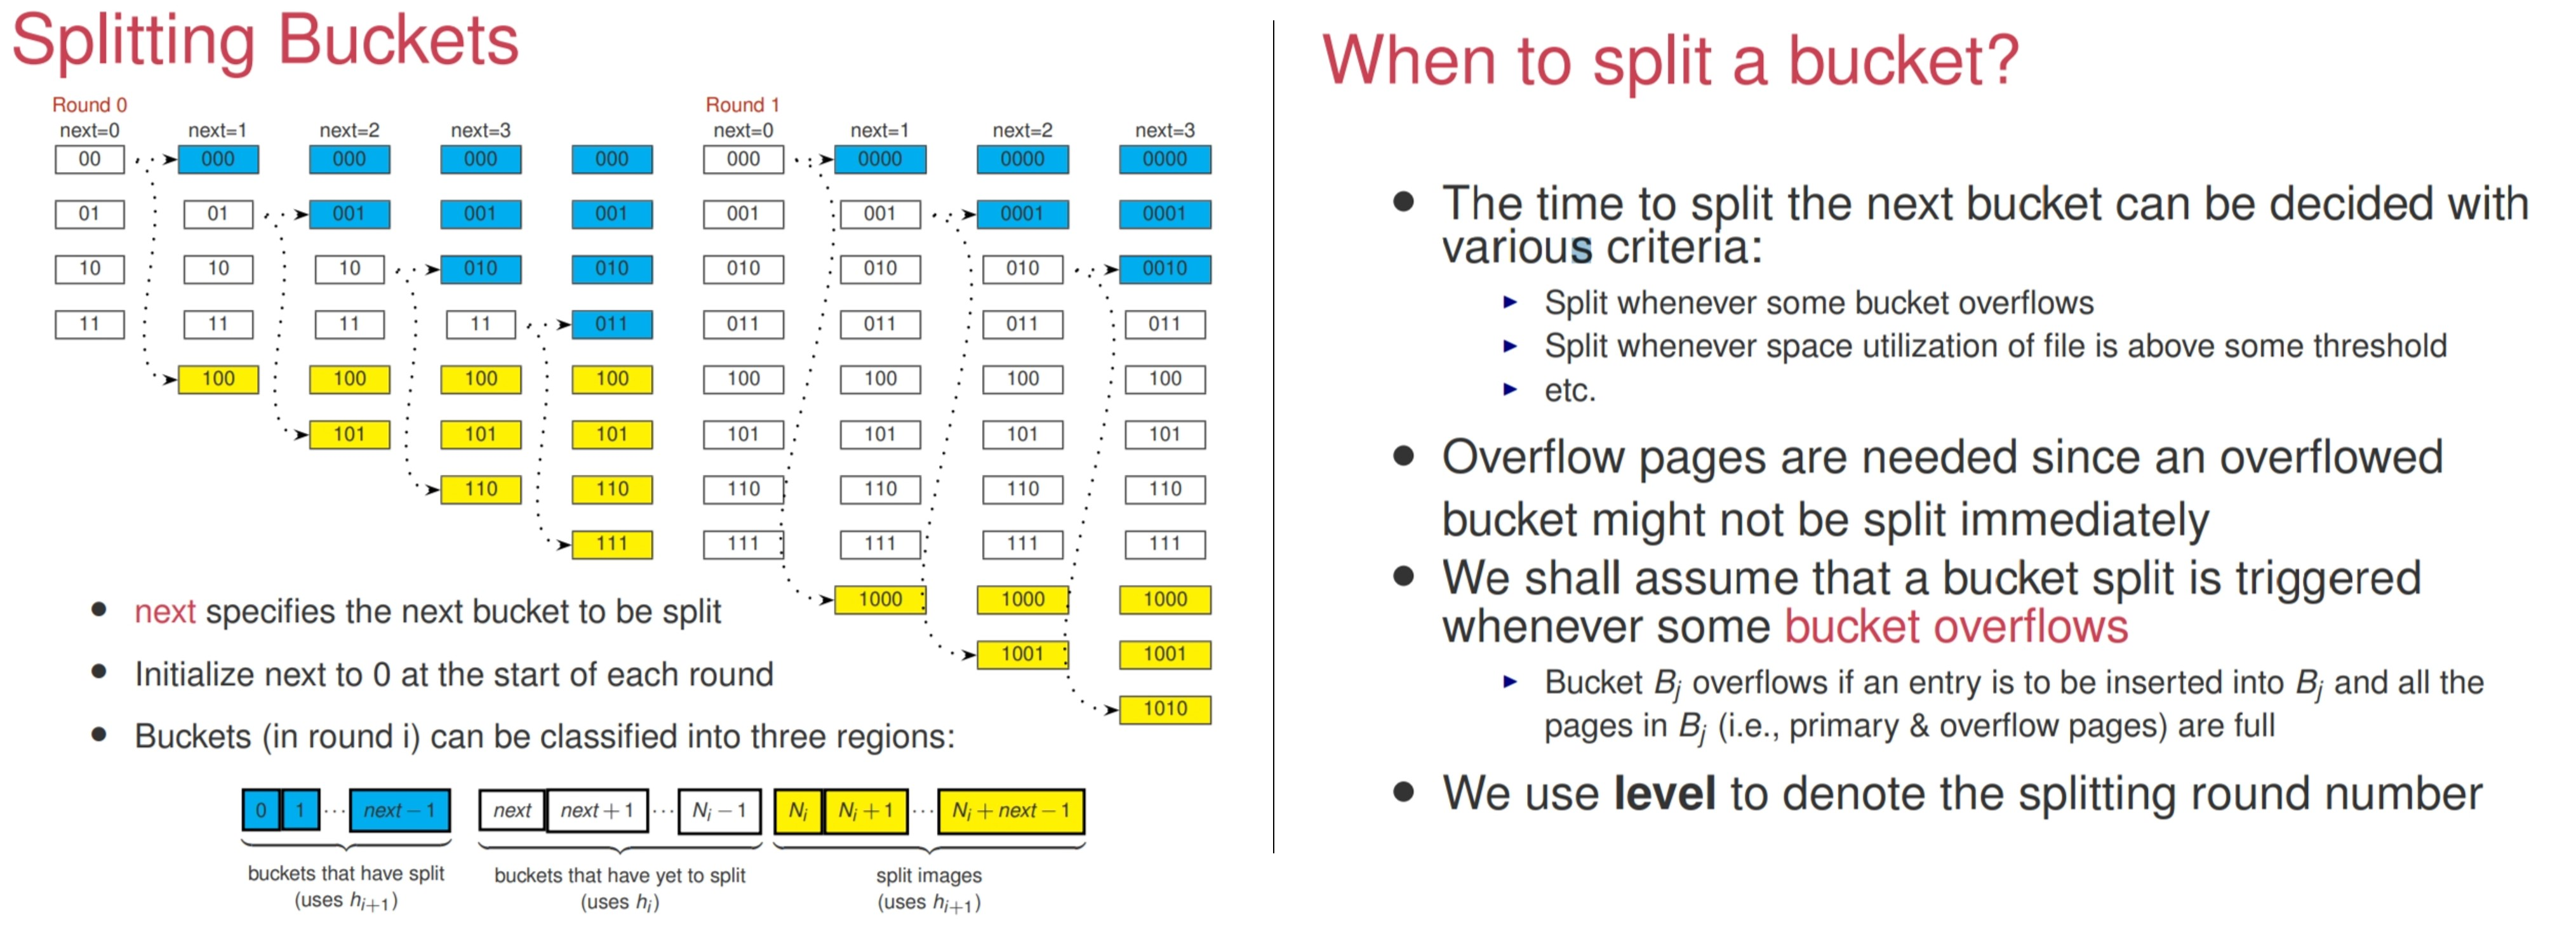
\includegraphics[width = 1\linewidth]{splitBucket}}

\subsubsection{Examples: Linear Hashing Search \& Insert}
\begin{itemize}
\item Even though overflowed bucket split, not necessary mean enough space if bit value not right. Still require overflow page.
\item Using \textbf{level and next}, we determine how many additional bits to consider in \textbf{second hashing function}.
\item \textbf{Second hashing function}: Is simply looking at the m rightmost bits of the hash.
\end{itemize}
\centerline{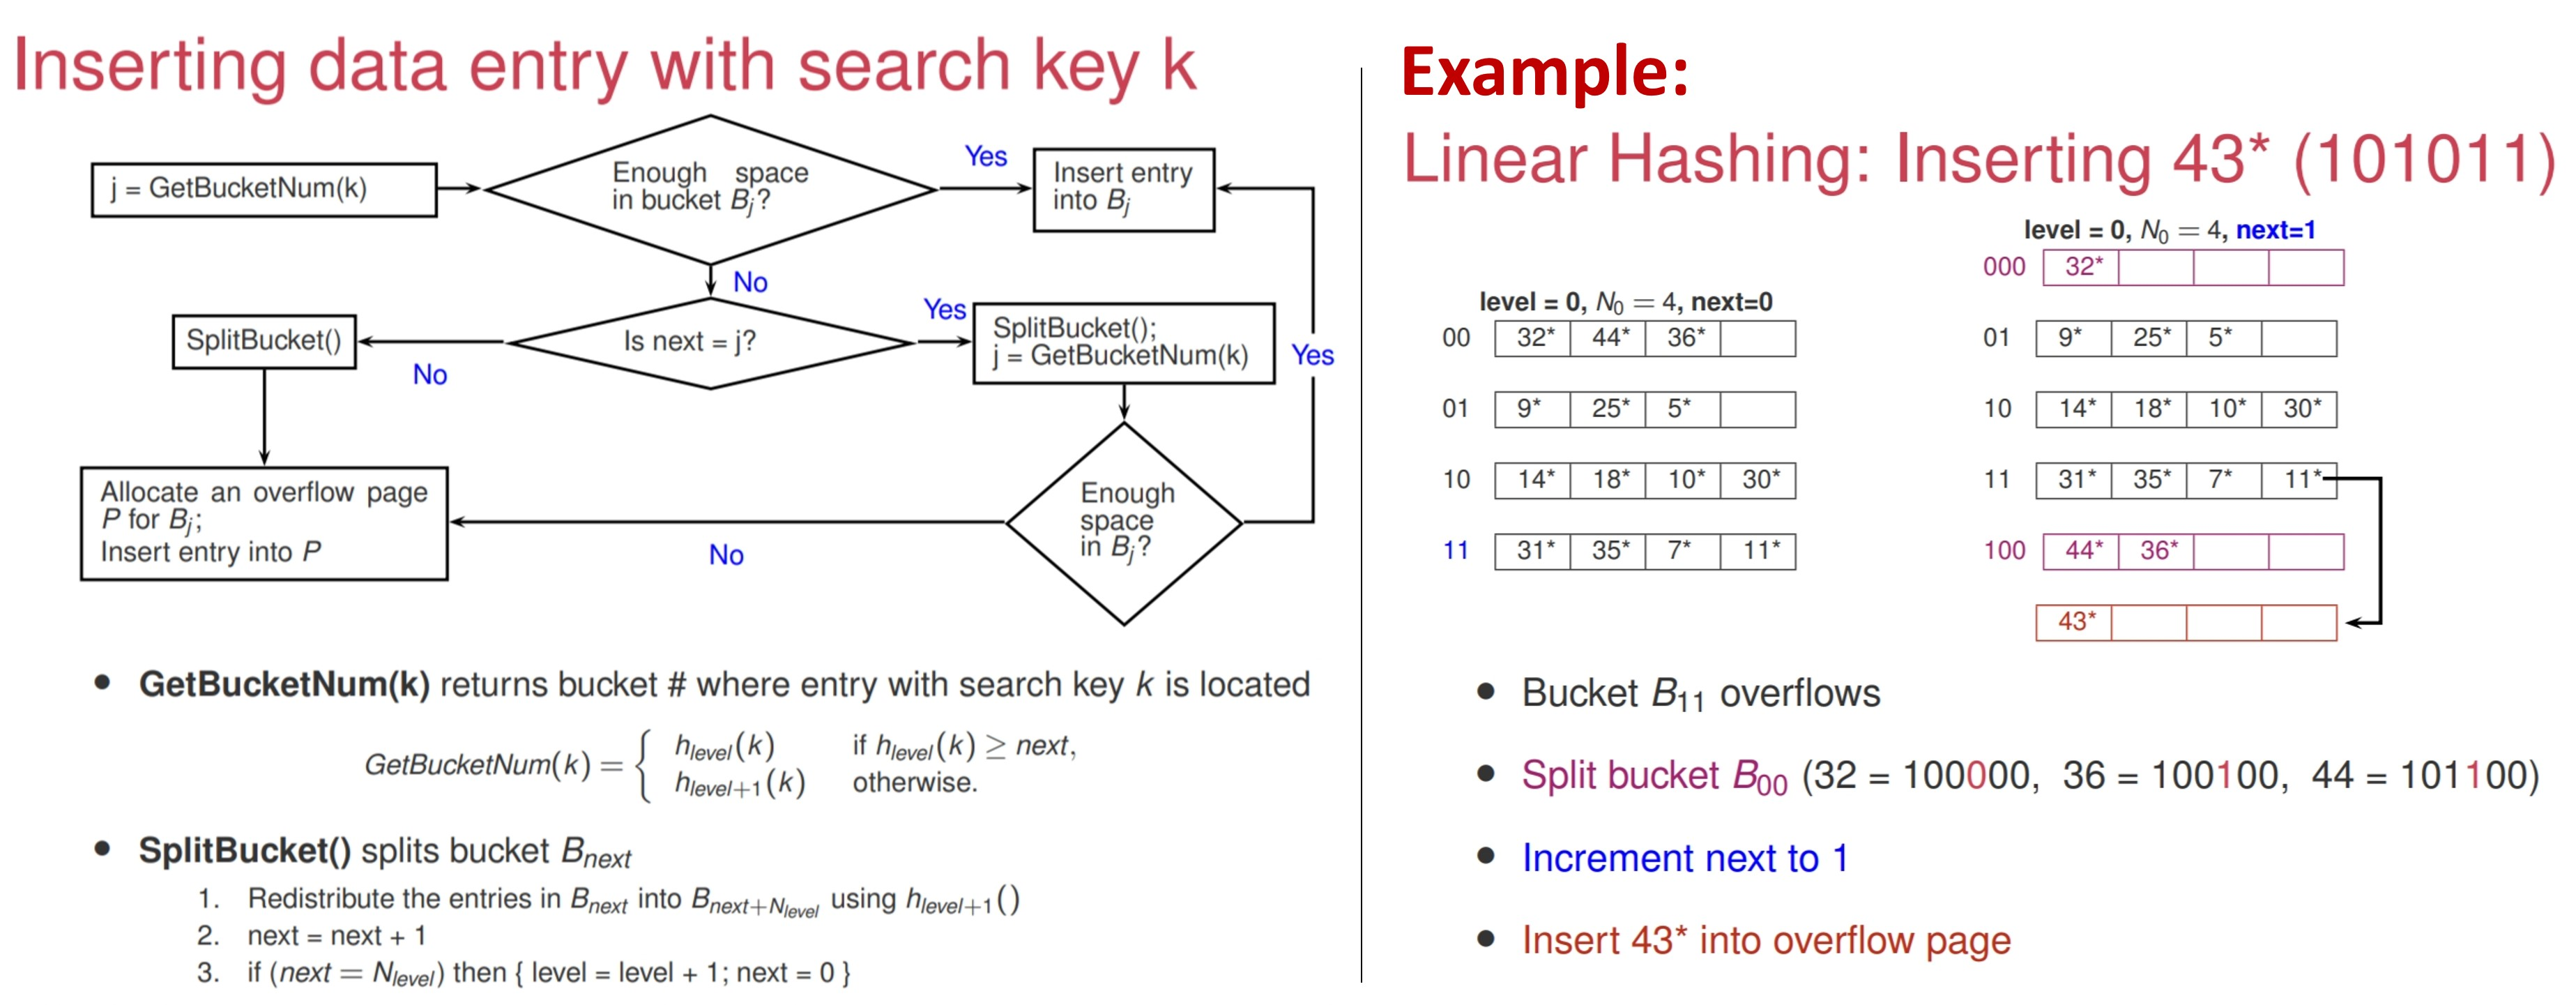
\includegraphics[width = 0.9\linewidth]{splitBucket1}}
\centerline{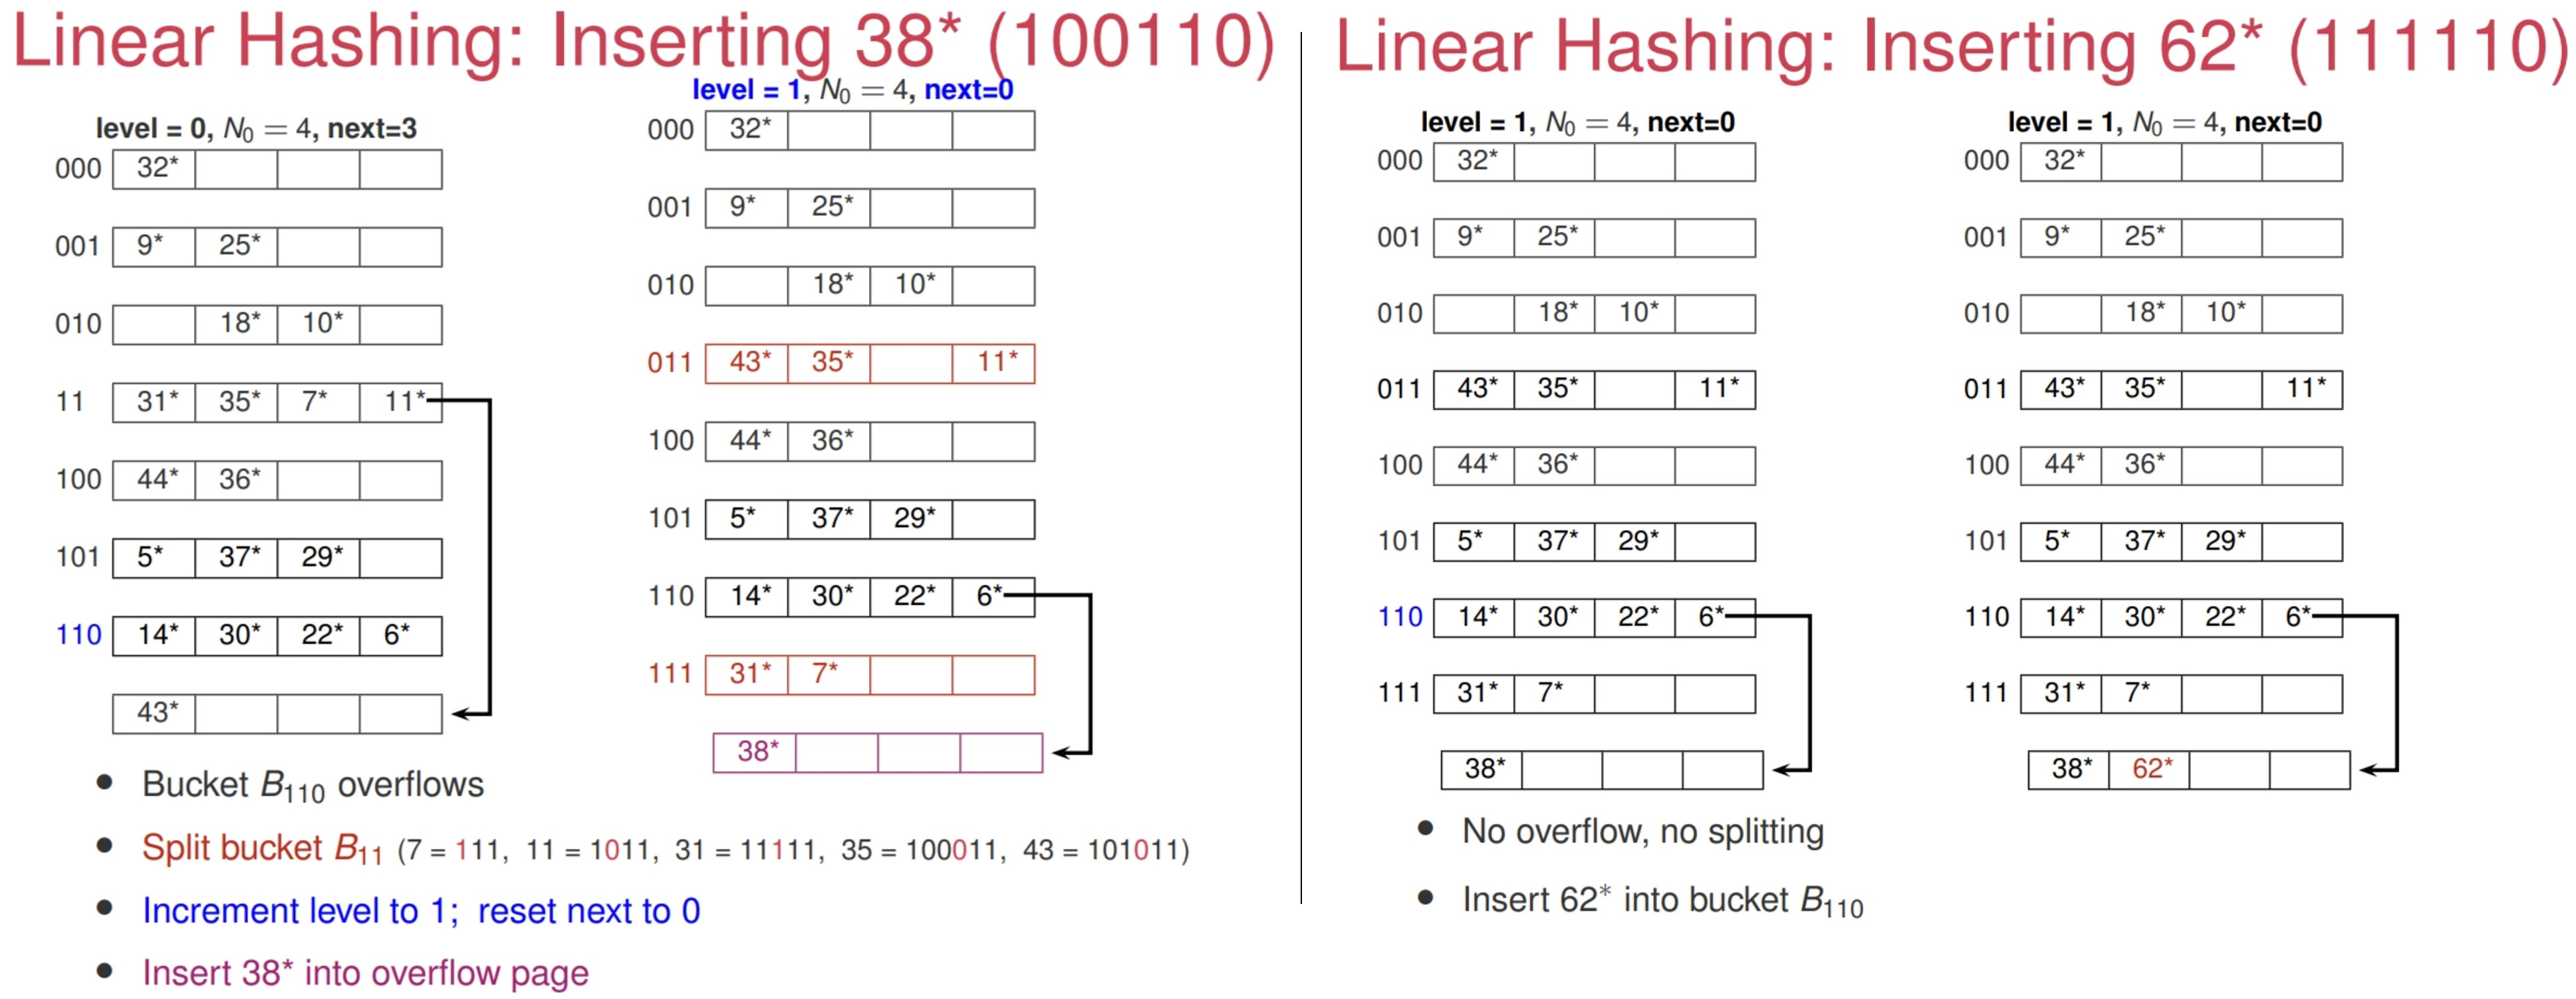
\includegraphics[width = 0.85\linewidth]{splitBucket2}}

\subsubsection{Linear Hashing Deletion}
\begin{itemize}
\item Opposite of insertion.
\item \textbf{Two cases}: 1. (Next > 0), 2. (Next = 0, and level $>$ 0.)
\end{itemize}
\centerline{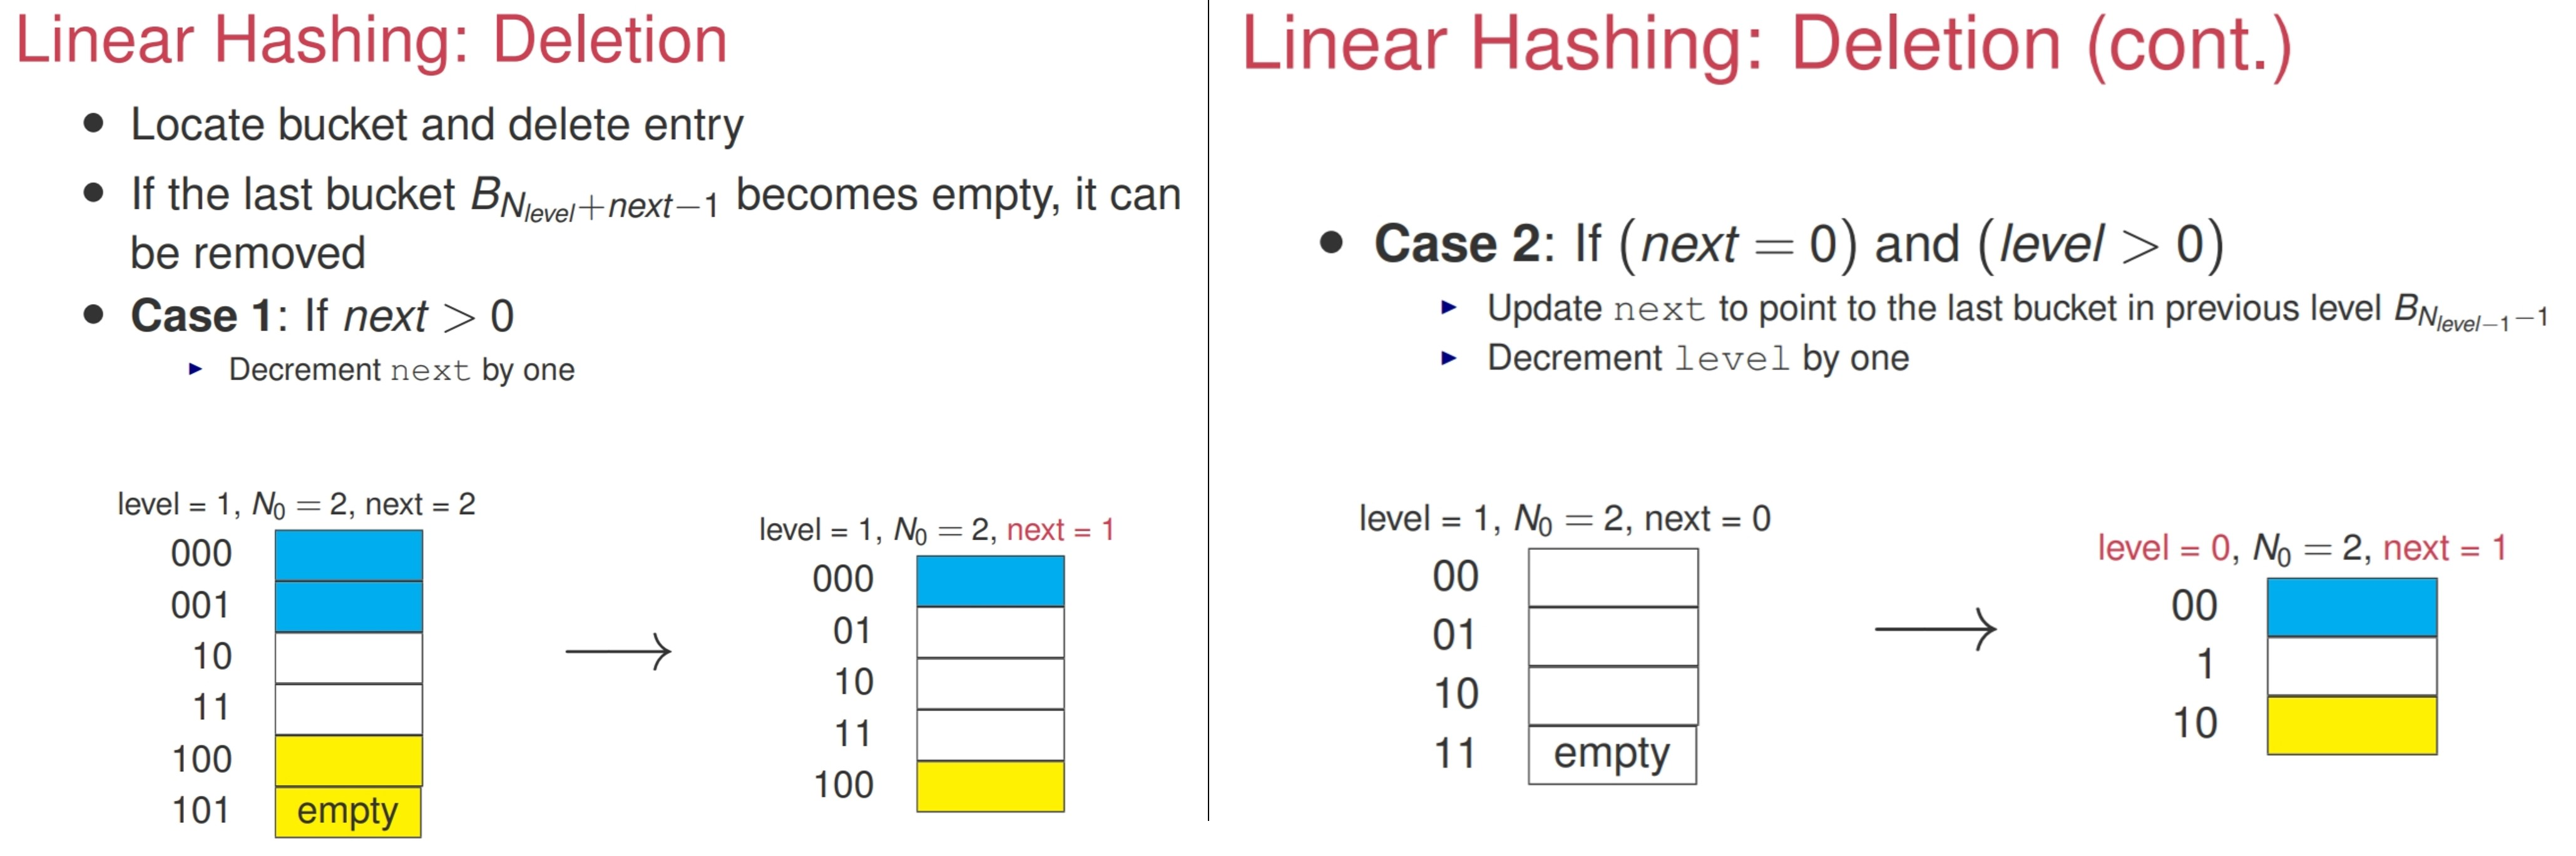
\includegraphics[width = 1\linewidth]{deletionBucket}}

\subsubsection{Linear Hashing Performance, Summary}
\centerline{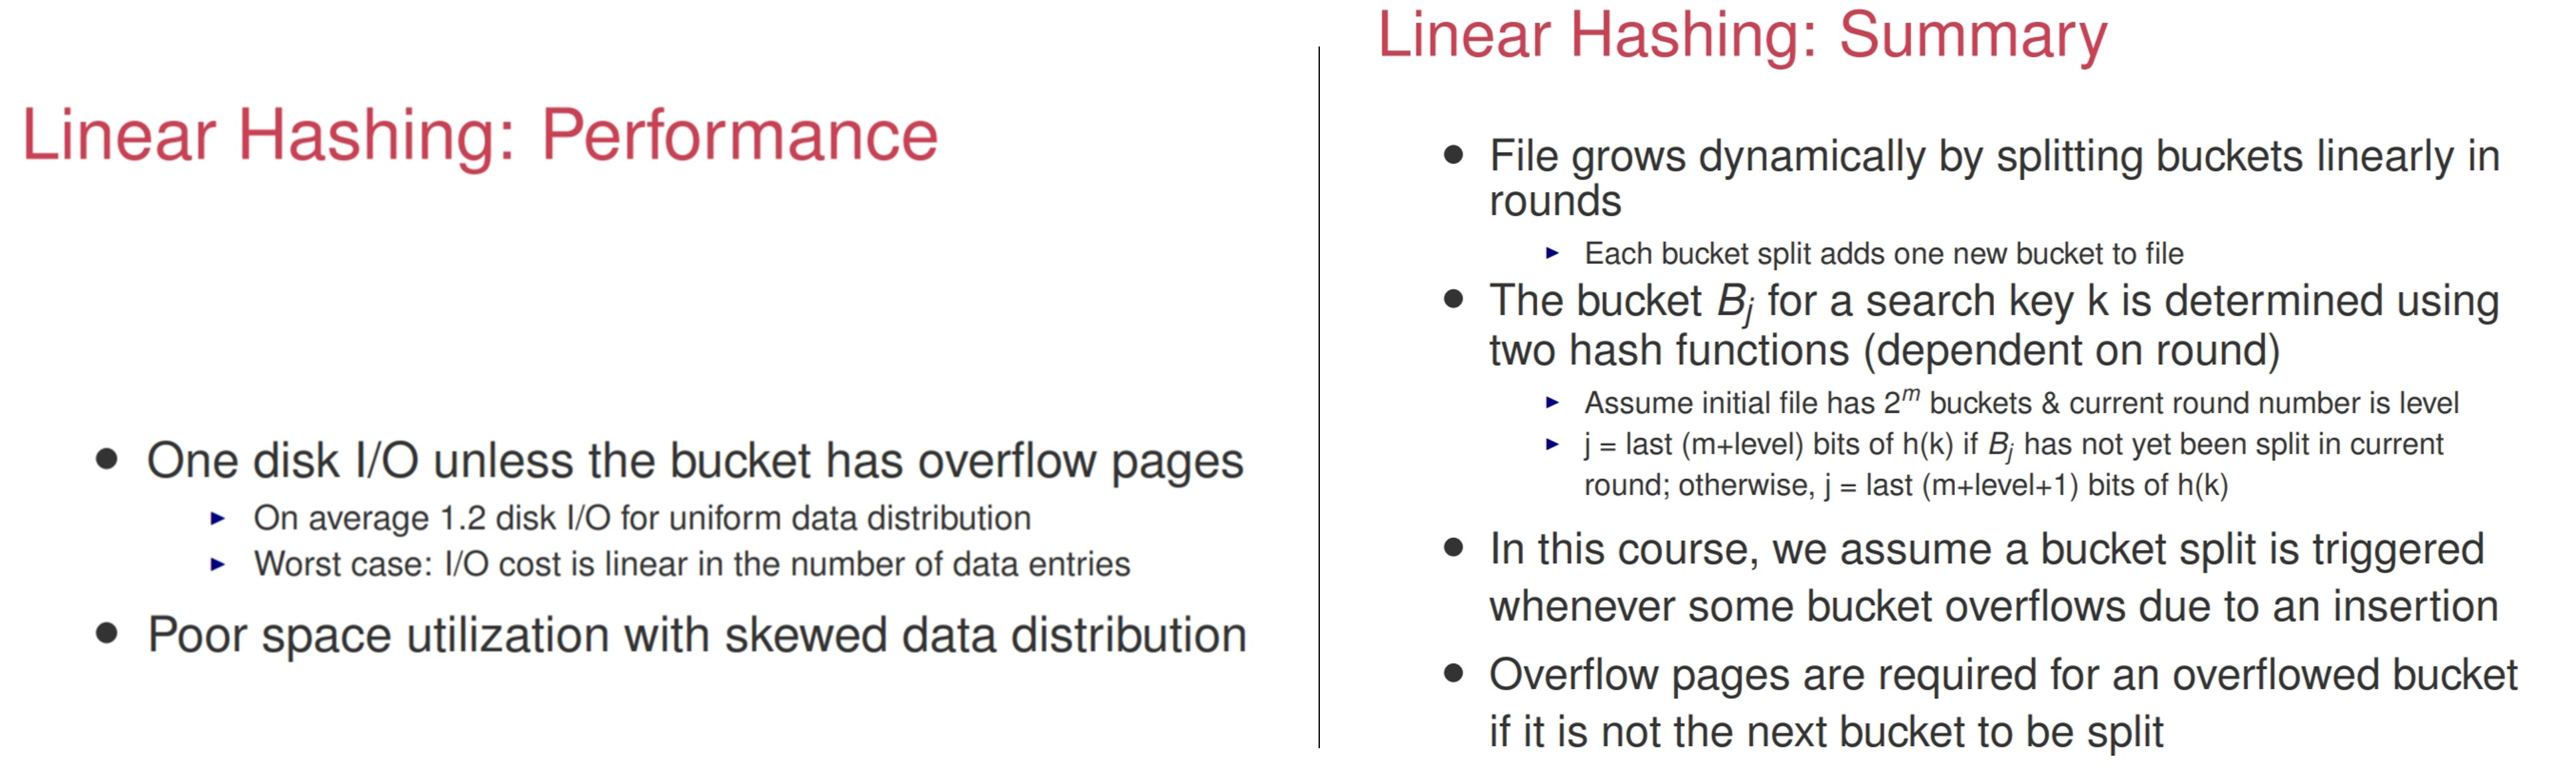
\includegraphics[width = 1\linewidth]{linearHashingSummary}}

\columnbreak

\subsection{Dynamic Hashing: Extendible Hashing}
\begin{itemize}
\item \textbf{Similar to Linear Hashing}: we want \textbf{bucket number to grow dynamically}, and use some \textbf{number of least significant bits} of h(k) to determine bucket address for search key $k$.
\item \textbf{Difference}: Add new bucket (as split image) when existing bucket overflows, No overflow pages (except when number of collisions exceed page capacity, two page entries collide if they have same h(.) hash value).
\end{itemize}

\subsection{Extendible Hashing}
\begin{itemize}
\item \textbf{Extendible hashing}: dynamically updatable disk-based index structure, implements hashing scheme utilizing a \textbf{directory of pointers to buckets}. 
\item Overflows handled by doubling the directory which logically doubles the number of buckets. \textbf{Physically, only the overflown bucket is split}.
\end{itemize}
\centerline{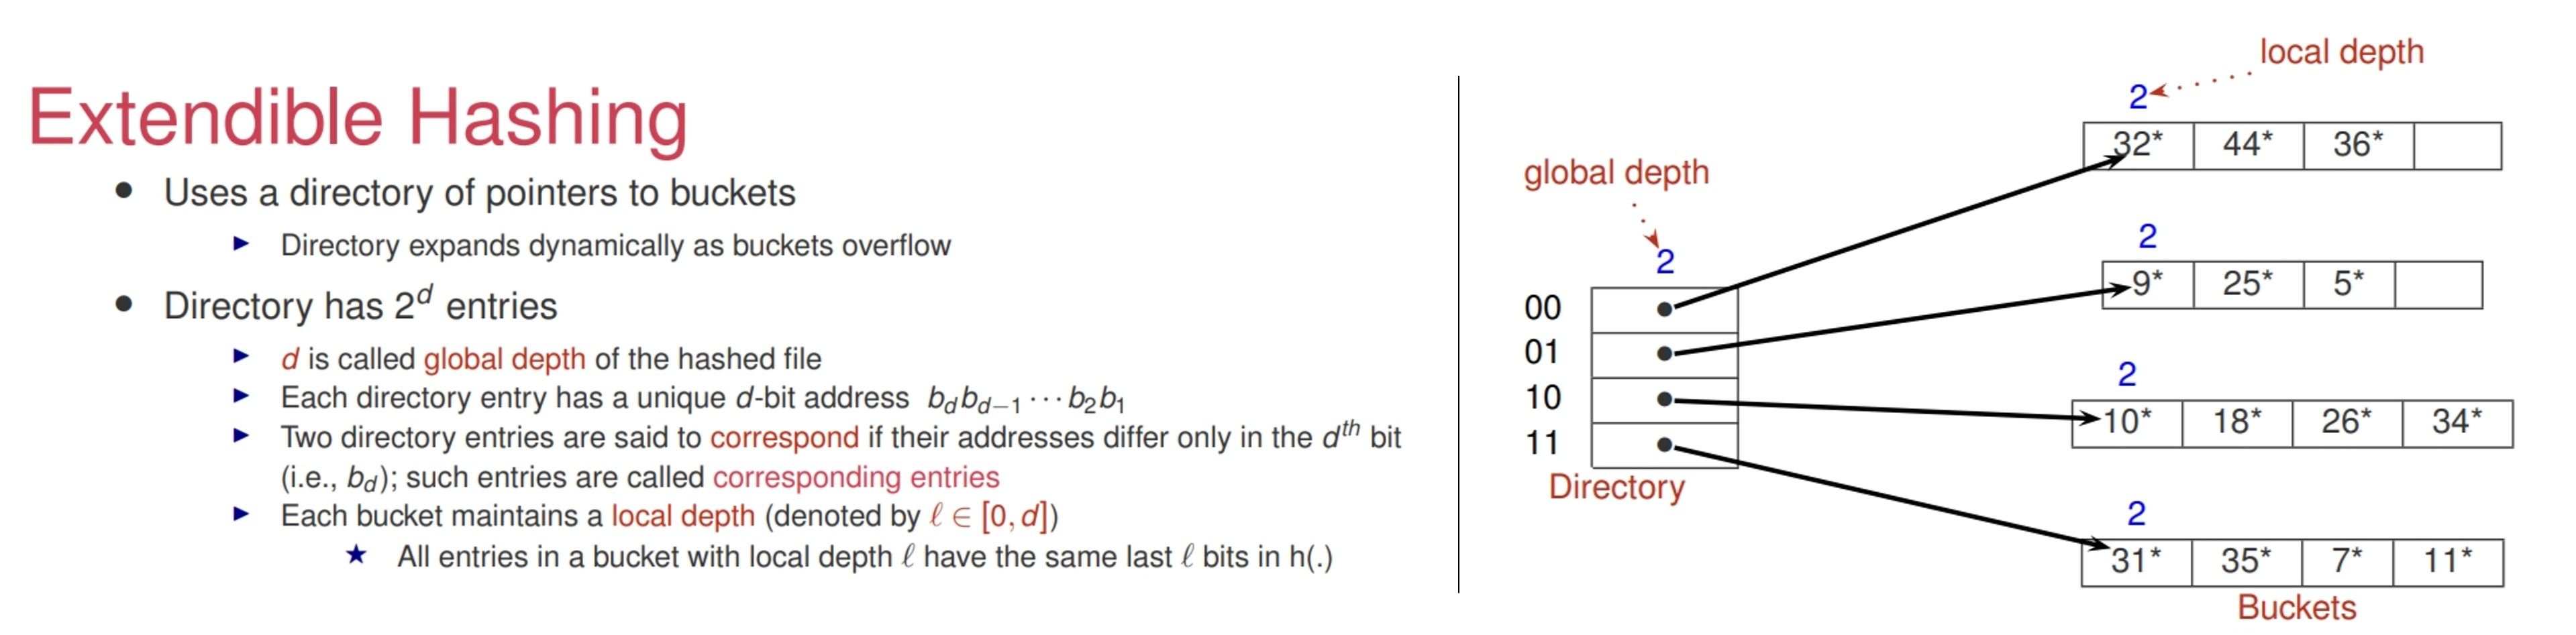
\includegraphics[width = 1\linewidth]{extendibleHashing}}

\subsubsection{Extendible Hashing Performance}
\begin{itemize}
\item \textbf{Performance}: At most 2 disk I/O for equality selection, at most 1 I/O if directory fits in main memory.
\item \textbf{Handling collision}: Two data entries \textbf{collide} if same hashed value, overflow pages need when number of collisions exceed page capacity.
\item Compared with B+-tree index exact match queries (log number of I/Os), E. Hashing better expected query cost O(1) I/O. 
\end{itemize}

\subsubsection{Extendible Hashing: Handling Bucket Overflow}
\begin{itemize}
\item Main idea: Determine if there is empty directory entry to point to new bucket. \textbf{2 Cases}: decision to split, or use empty directory entry.
\end{itemize}

\subsubsection{Case 1: Split bucket local depth = global depth}
\centerline{\includegraphics[width = 1\linewidth]{extendibleHashing1}}

\subsubsection{Case 2: Split bucket local depth $<$ global depth.}
\centerline{\includegraphics[width = 1\linewidth]{extendibleHashing2}}

\columnbreak

\subsubsection{Extendible Hashing Deletion}
\begin{itemize}
\item To delete entry, simply locate Bucket and delete. 
\item \textbf{Merging}: Mergable if entries can fit within a bucket, and same local depth, $j$ differs on in $l^{th}$ bit.
\end{itemize}
\centerline{\includegraphics[width = 1\linewidth]{extendibleHashing3}}

\section{4. Query Evaluation: Sorting \& Selection}
DBMS describes data it manages using tables, indexes (metadata), which is stored in special tables (system catalogs). This data used to find best way to evaluate a query.
\centerline{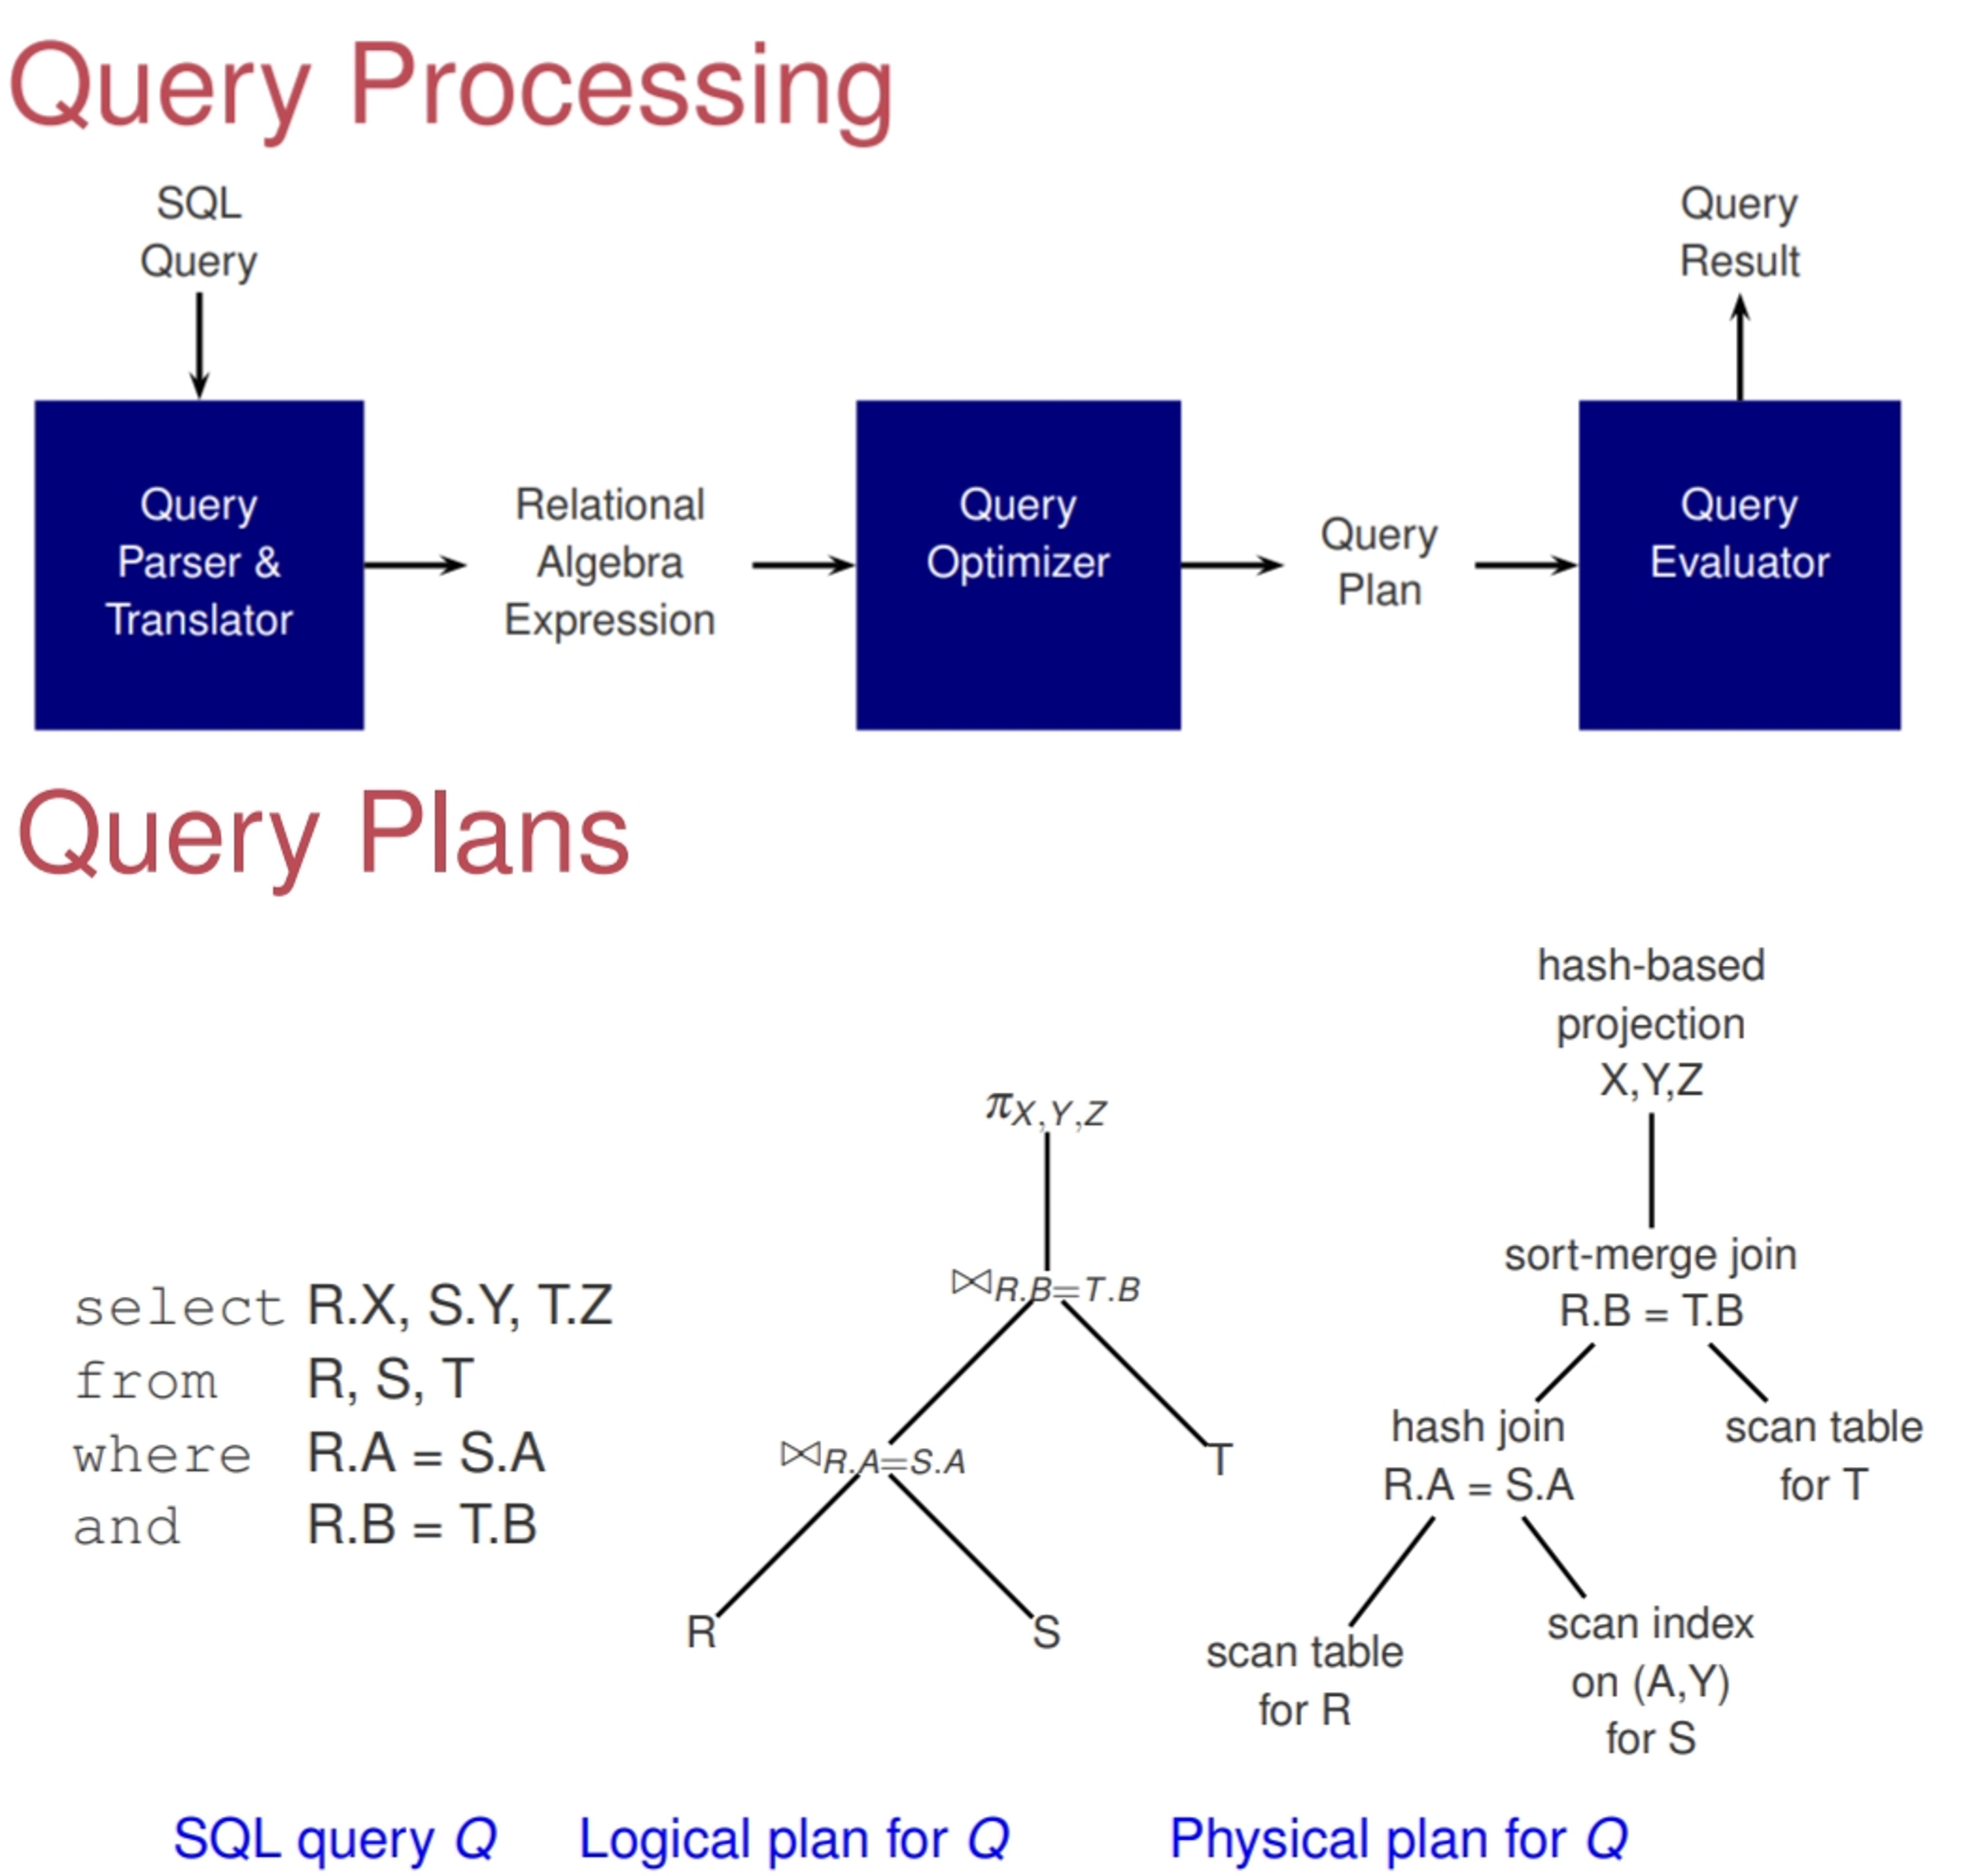
\includegraphics[width = 0.8\linewidth]{queryProcessing}}
\begin{itemize}
\item SQL queries translate into extended form of relational algebra
\item Query evaluation plans represented as tree of relational operators, with labels identifying algorithm to use at each node.
\item R. operators building blocks for evaluating queries, implementation of operators optimized for good perf.
\end{itemize}

\section{External Sorting}
Sorting collection of records on some (search) key is useful and required in variety of situations, including 
\begin{itemize}
\item Some sorted table of results: \code{SELECT * FROM student ORDER BY age}.
\item Bulk loading a $B^+$-tree index
\item Implementation of other relational algebra operators (e.g. projection, join), which require some sorting step.
\end{itemize}
When data to be sorted too large to fit into available main memory. Need some \textbf{external sorting algorithm}. Algos seek to minimize cost of disk accesses.

\subsection{External Merge Sort}
\begin{itemize}
\item \textbf{Main Idea}: Pass 0: Creating initial sorted runs (each of X memory pages), then continue during merging passes till you get final sorted pass.
\item Sort entire fire by breaking into smaller subfiles, sorting subfiles and merging using minimal amount of main memory at given time.
\item \textbf{Each sorted subfile is referred to as a run}.
\item Sorting 11-page data R using 3 vs 4 memory pages:
\end{itemize}
\centerline{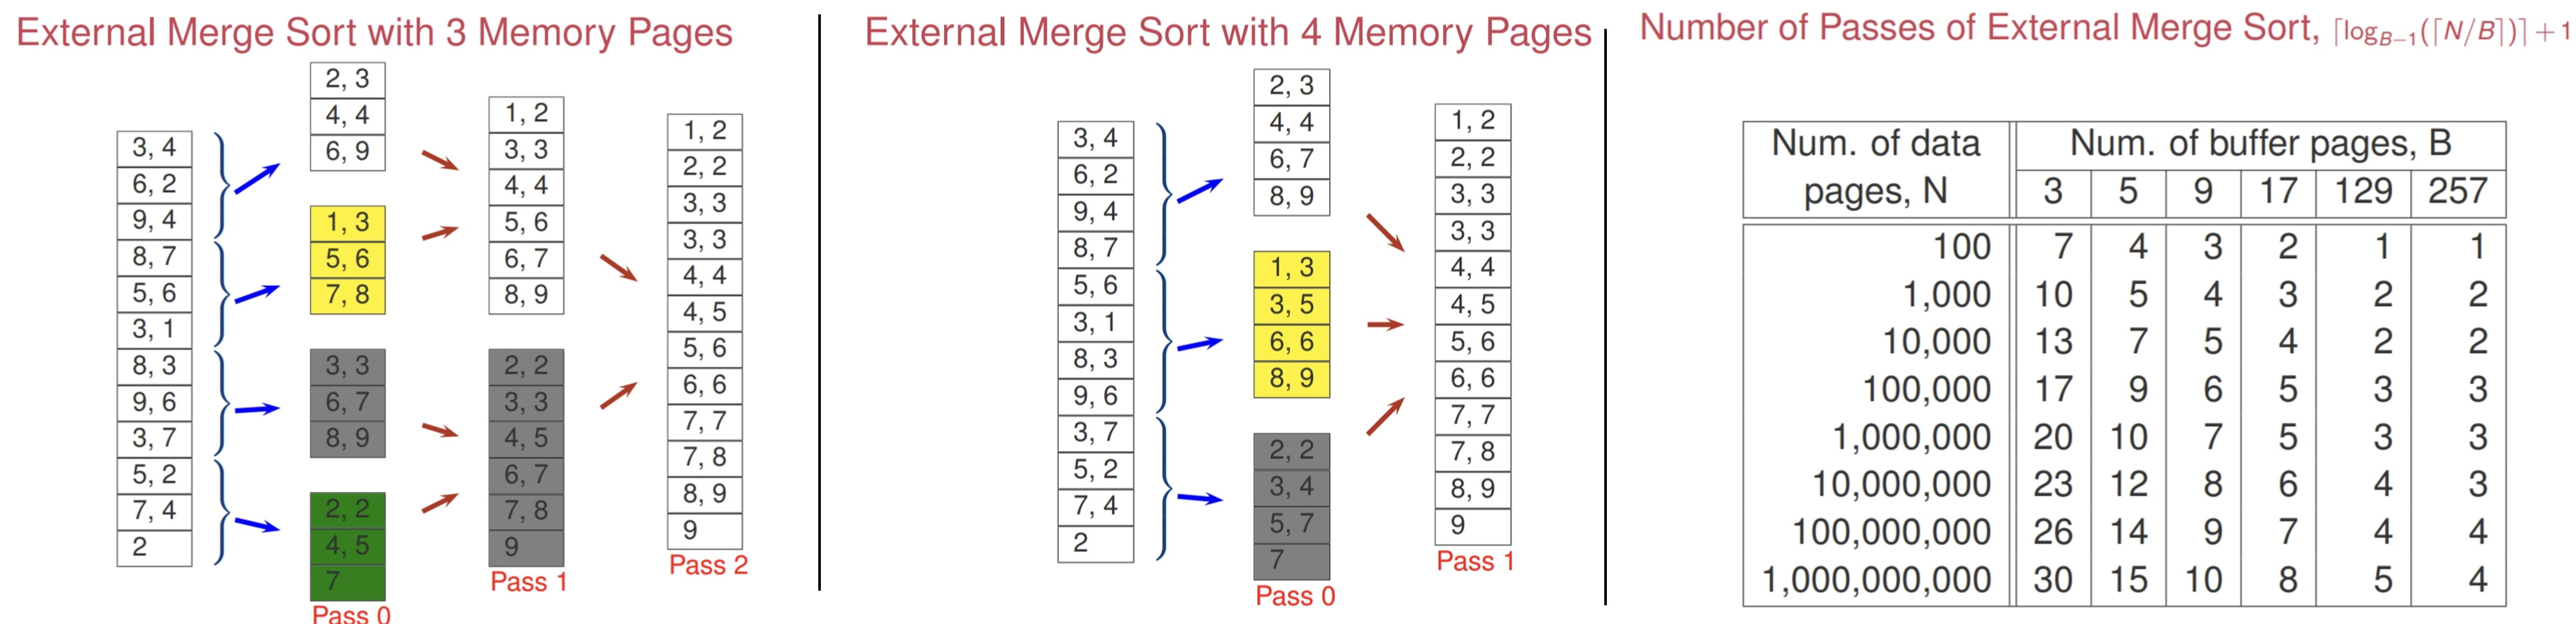
\includegraphics[width = 1\linewidth]{externalMergeSortExample}}
\subsection{External Merge Sort Analysis}
\begin{itemize}
\item \textbf{Note}: We consider only I/O costs, which approx by counting no. of pages read/written as per cost model. (Simple cost model to convey main idea).
\end{itemize}
\centerline{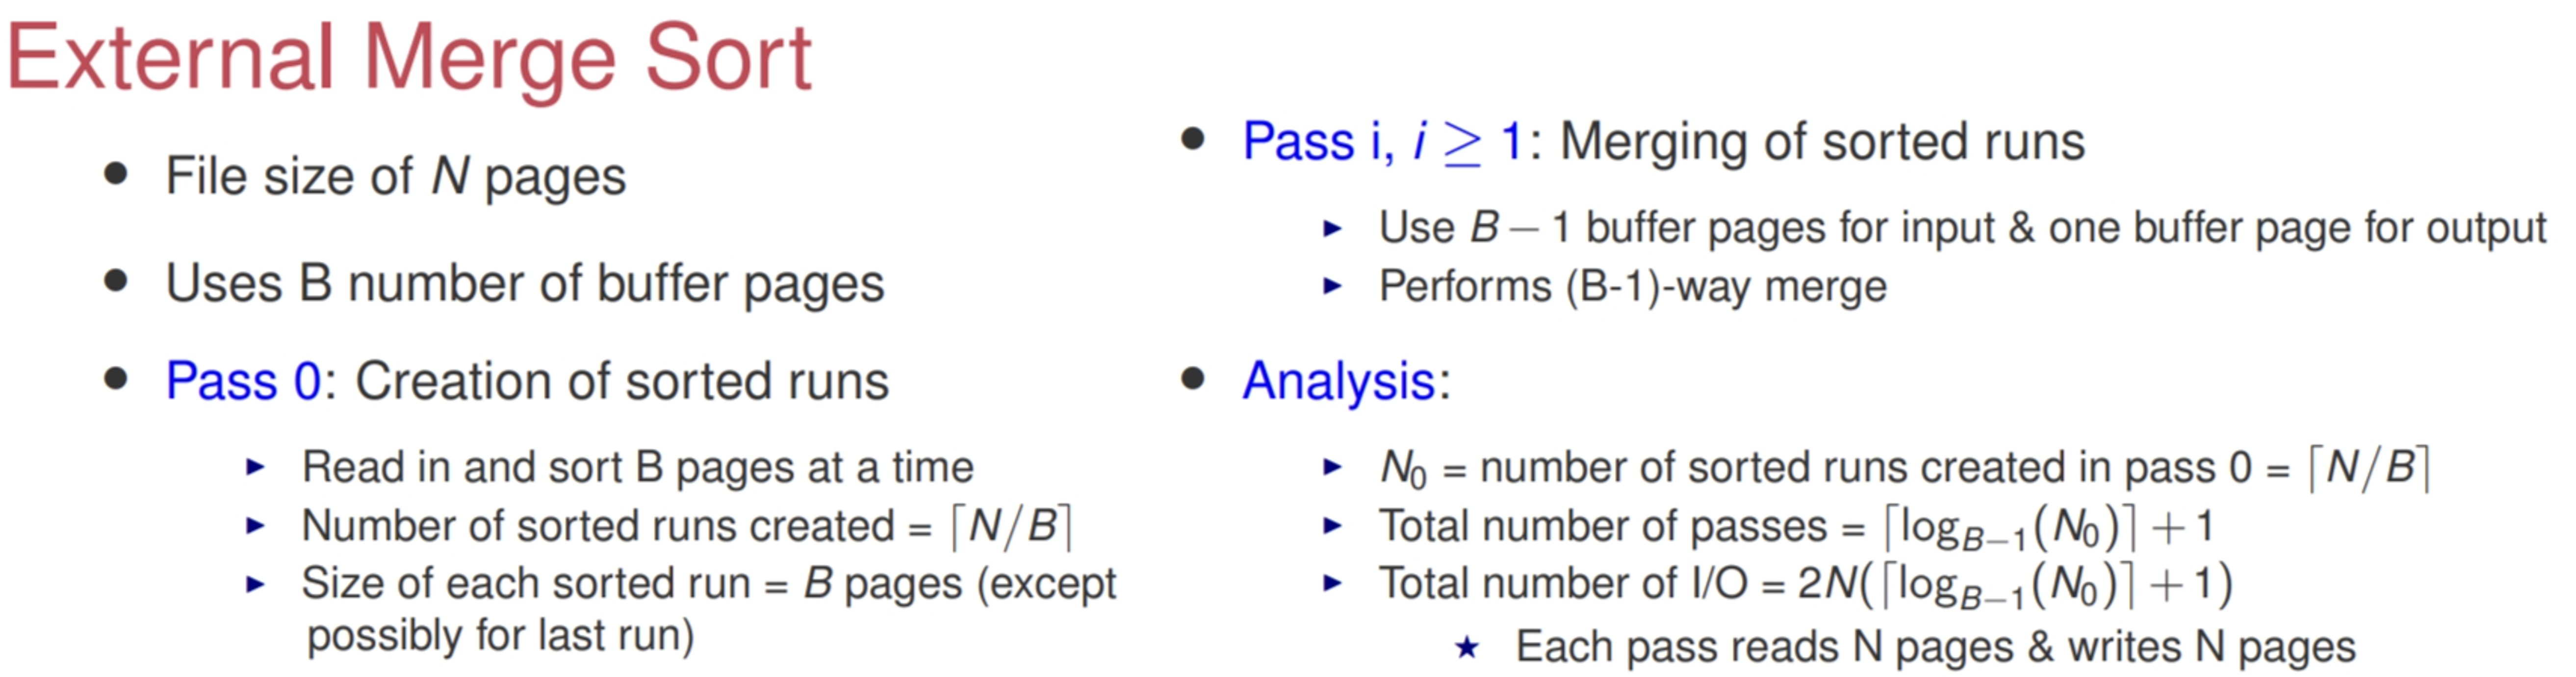
\includegraphics[width = 1\linewidth]{externalMergeSortSummary}}


\subsubsection{External Merge Sort Steps}
\centerline{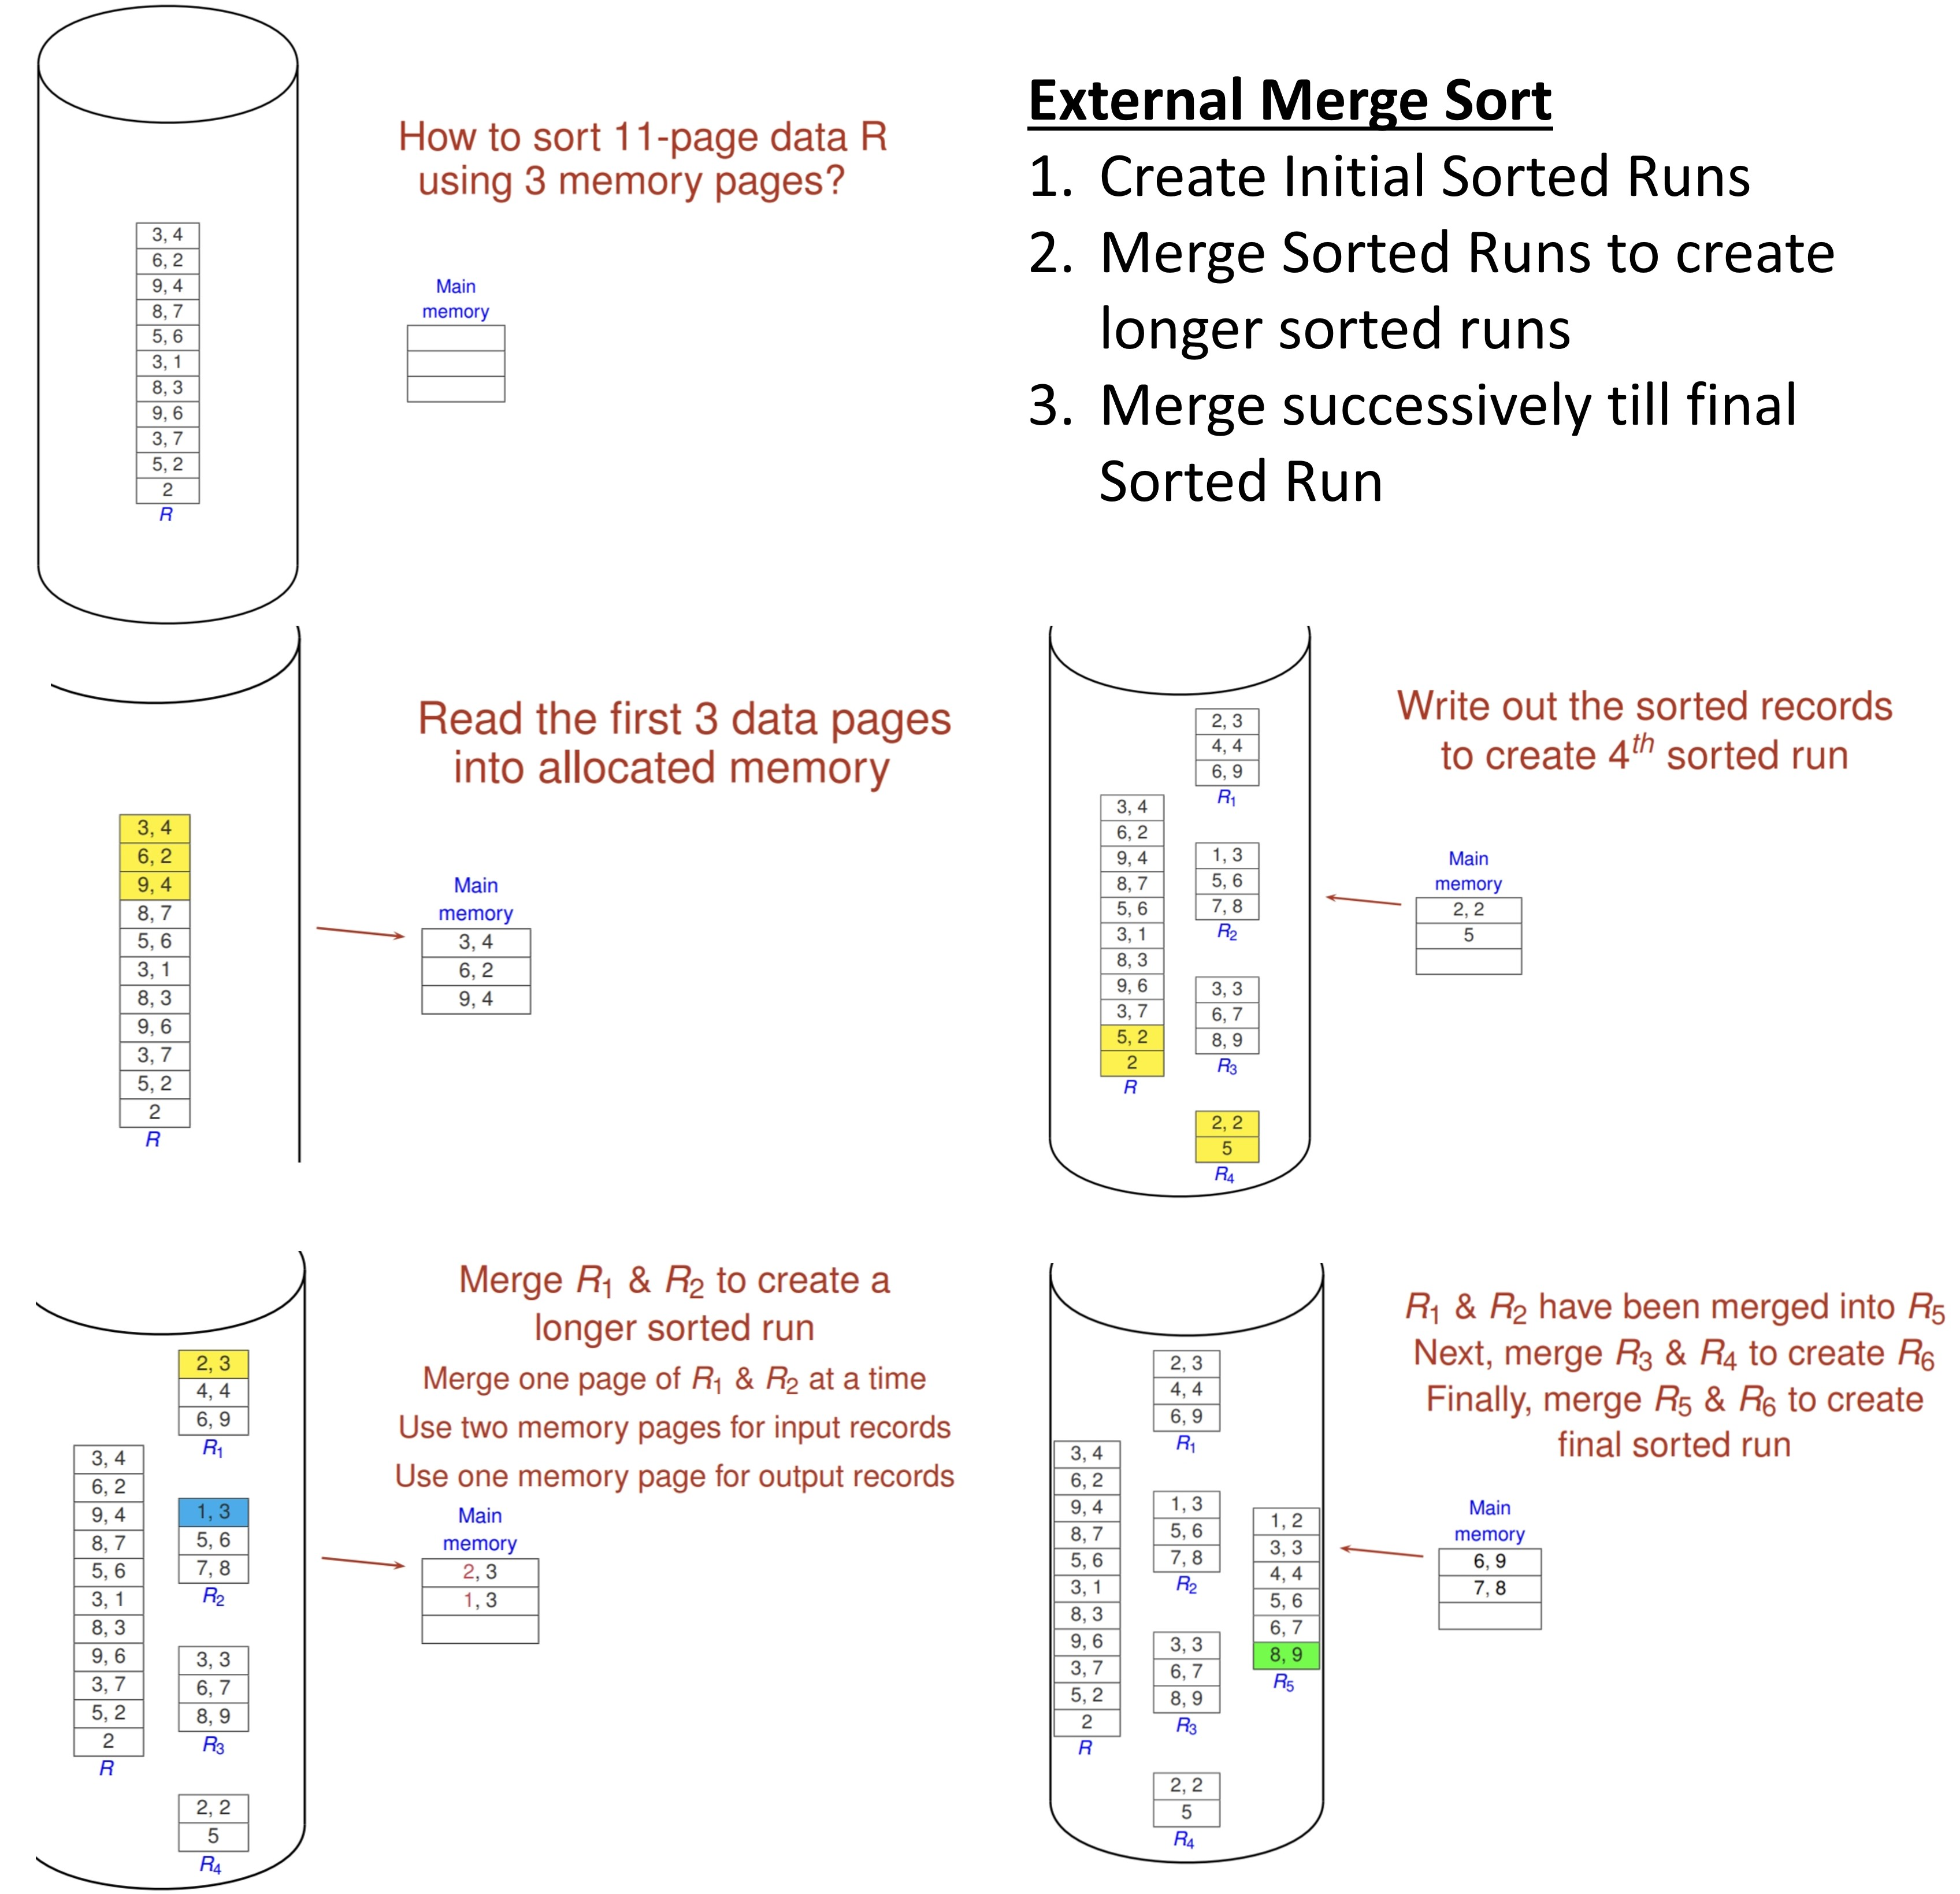
\includegraphics[width = 1\linewidth]{externalMergeSort}}

\columnbreak

\subsection{External Sort Optimization: I/O Cost vs. No. of I/Os}
\begin{itemize}
\item \textbf{Cost Metric}: No. of page I/Os. 
\item Only an approx of true I/O costs, ignores effect of \textbf{block(ed)} I/O, \textbf{single request to read/write several consecutive pages can be cheaper} than read/write same number of pages through independent I/O requests.
\item \textbf{Others}: Consider CPU costs as well, can use \textit{double buffering} to keep CPU busy while I/O op. in progress.
\end{itemize}

\subsection{External Sort, Block(ed) Page I/O Optimization}
\subsubsection{Non-Block(ed) Page I/O}
\begin{itemize}
\item \textbf{Consider only No. of page I/O as metric}: Minimize no. of passes in sorting, as each page in file read and written in each pass. 
\item This means we maximise fan-in \textbf{during merging} (aka, how many runs merged per pass), allocate just one buffer pool page per run, and one buffer page for output of merge.
\item Hence, (B-1)-way merge per run, minimizing number of passes in sorting algorithm.
\end{itemize}

\subsubsection{Block(ed) Page I/O}
\begin{itemize}
\item \textbf{Optimization}: Access in blocks may reduce average cost to read/write single page, consideration to read/write in units of more than one page, or R/W in units of a \textbf{buffer block}.
\item \textbf{Buffer block}, of \textbf{$b$ pages}. \textbf{$B$ is total number of buffer pages} for sorting. 
\end{itemize}
\centerline{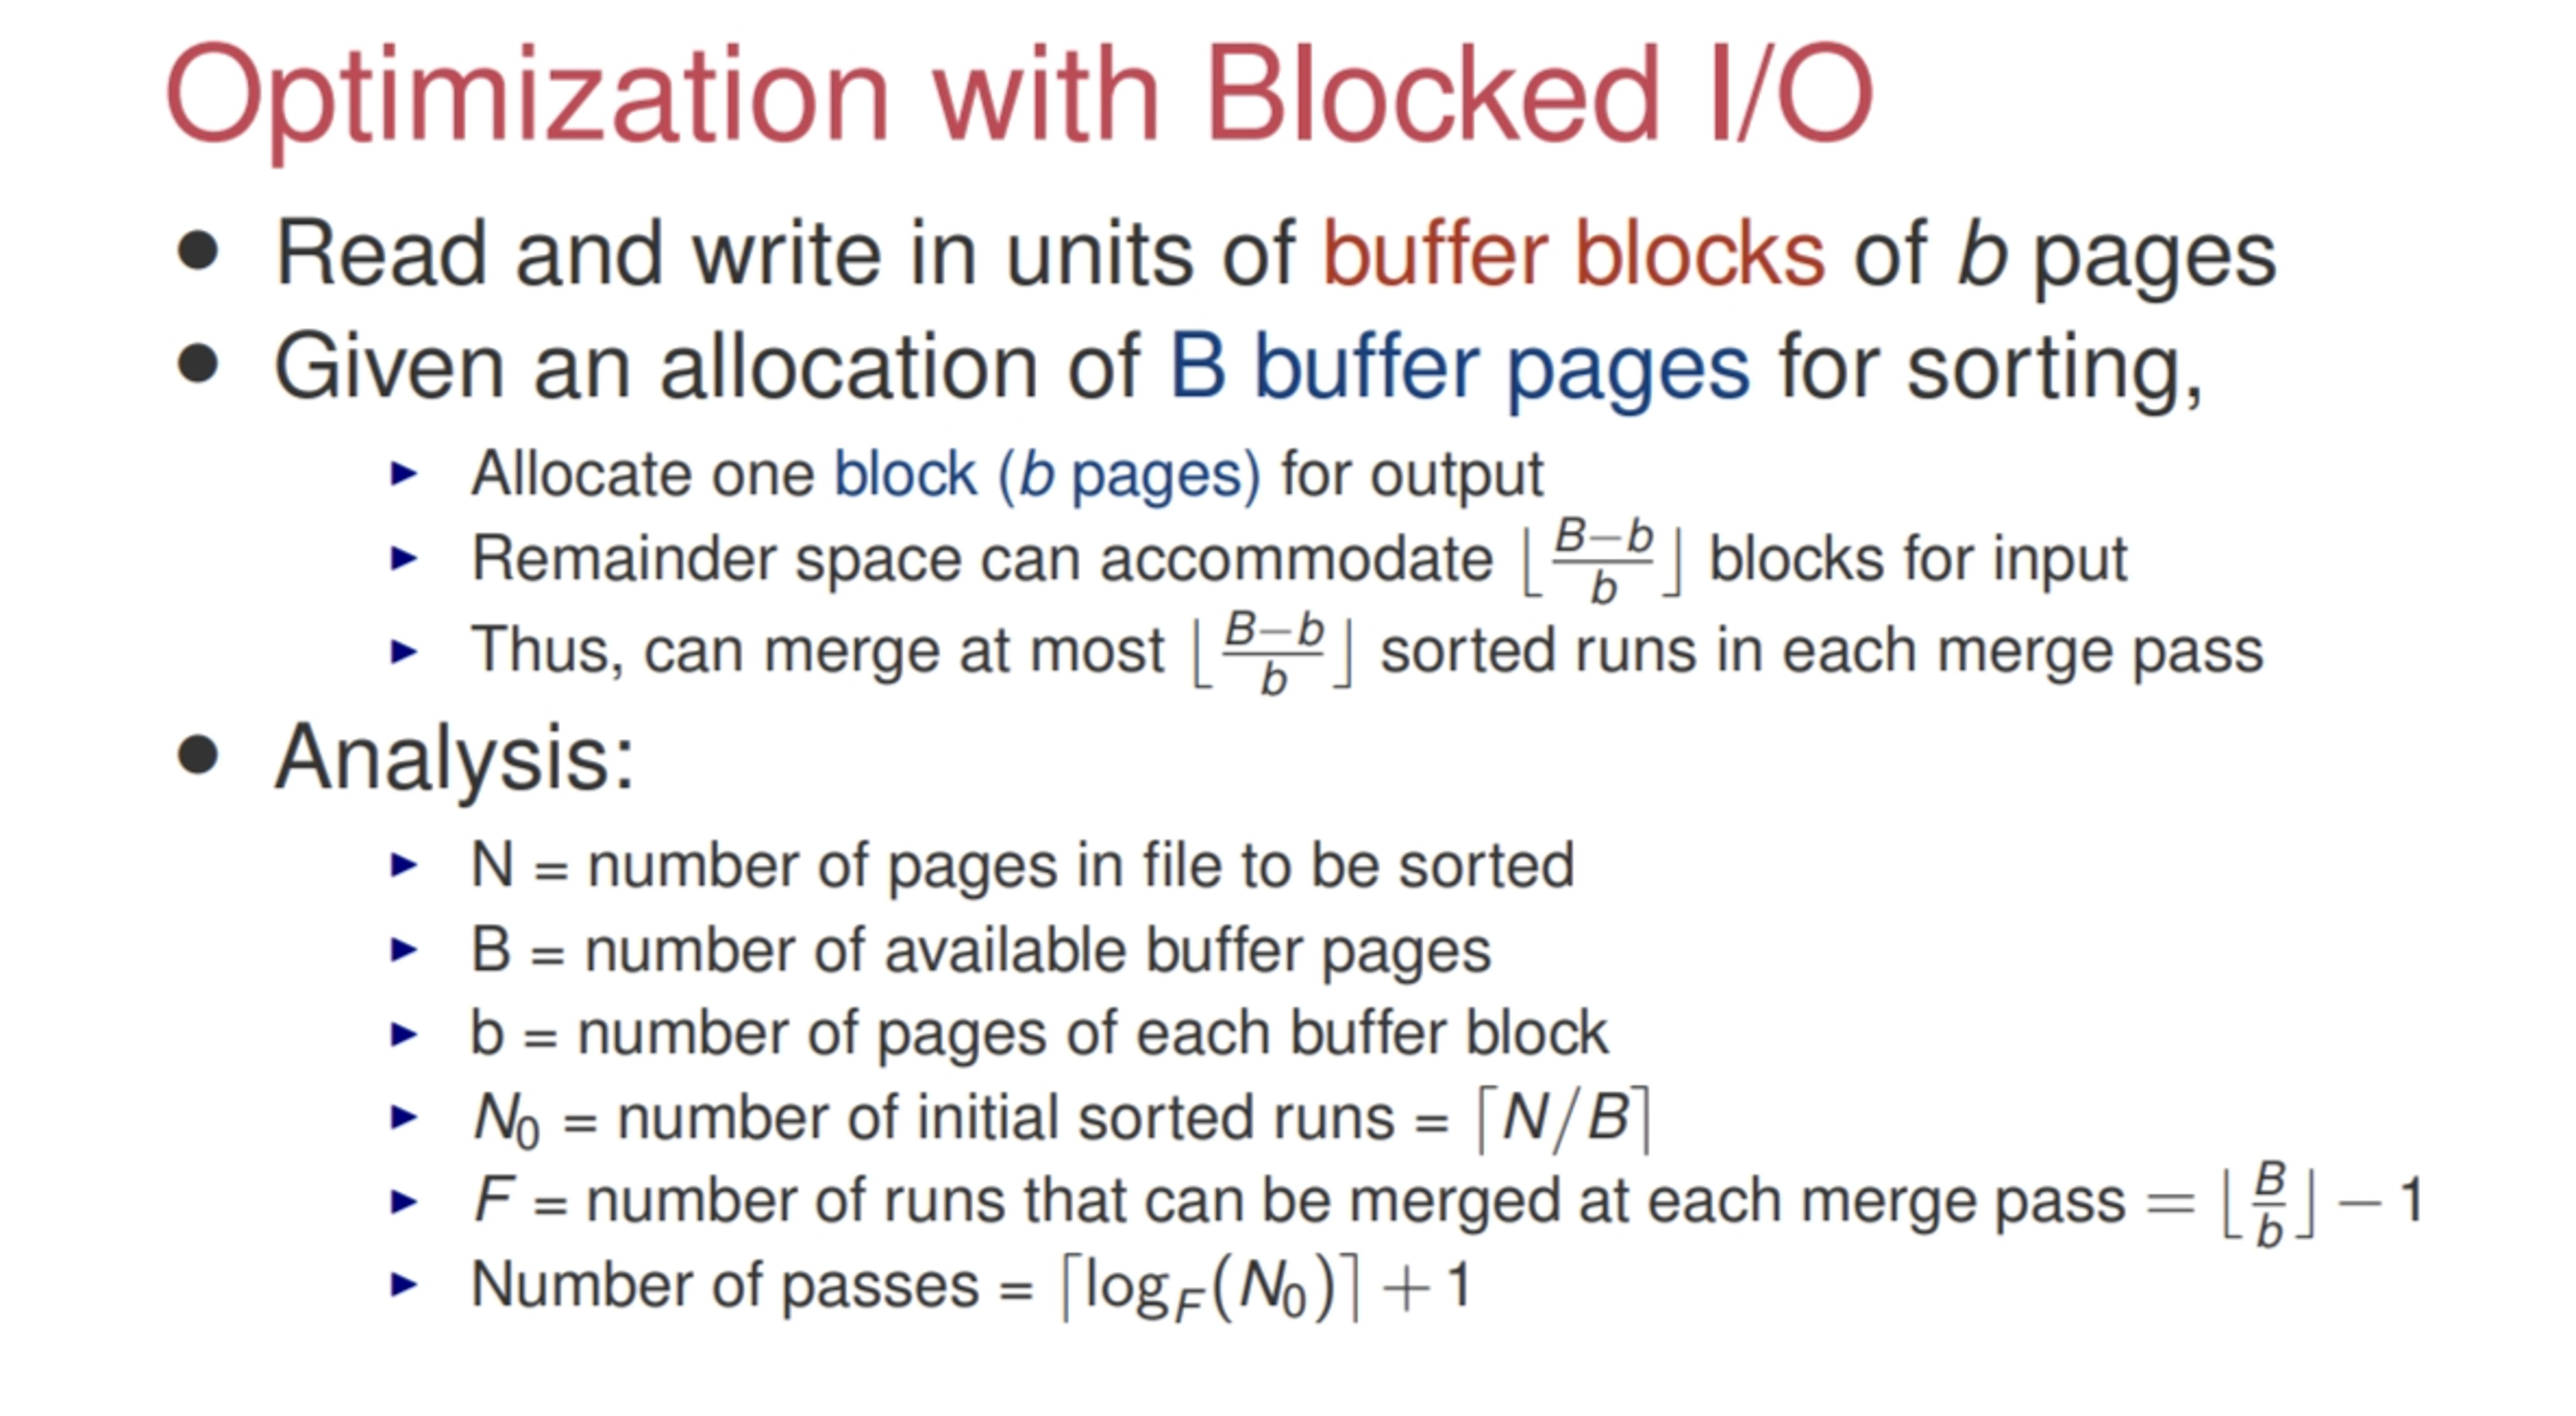
\includegraphics[width = 0.6\linewidth]{blockedIO}}
\begin{itemize}
\item Set aside one buffer block for output of merge. ($B-b$). One buffer block per input run ($\frac{B-b}{b}$). 
\item \textbf{Means can merge} at most floor($\frac{B-b}{b}$) sorted runs in each merge pass.
\end{itemize}
\centerline{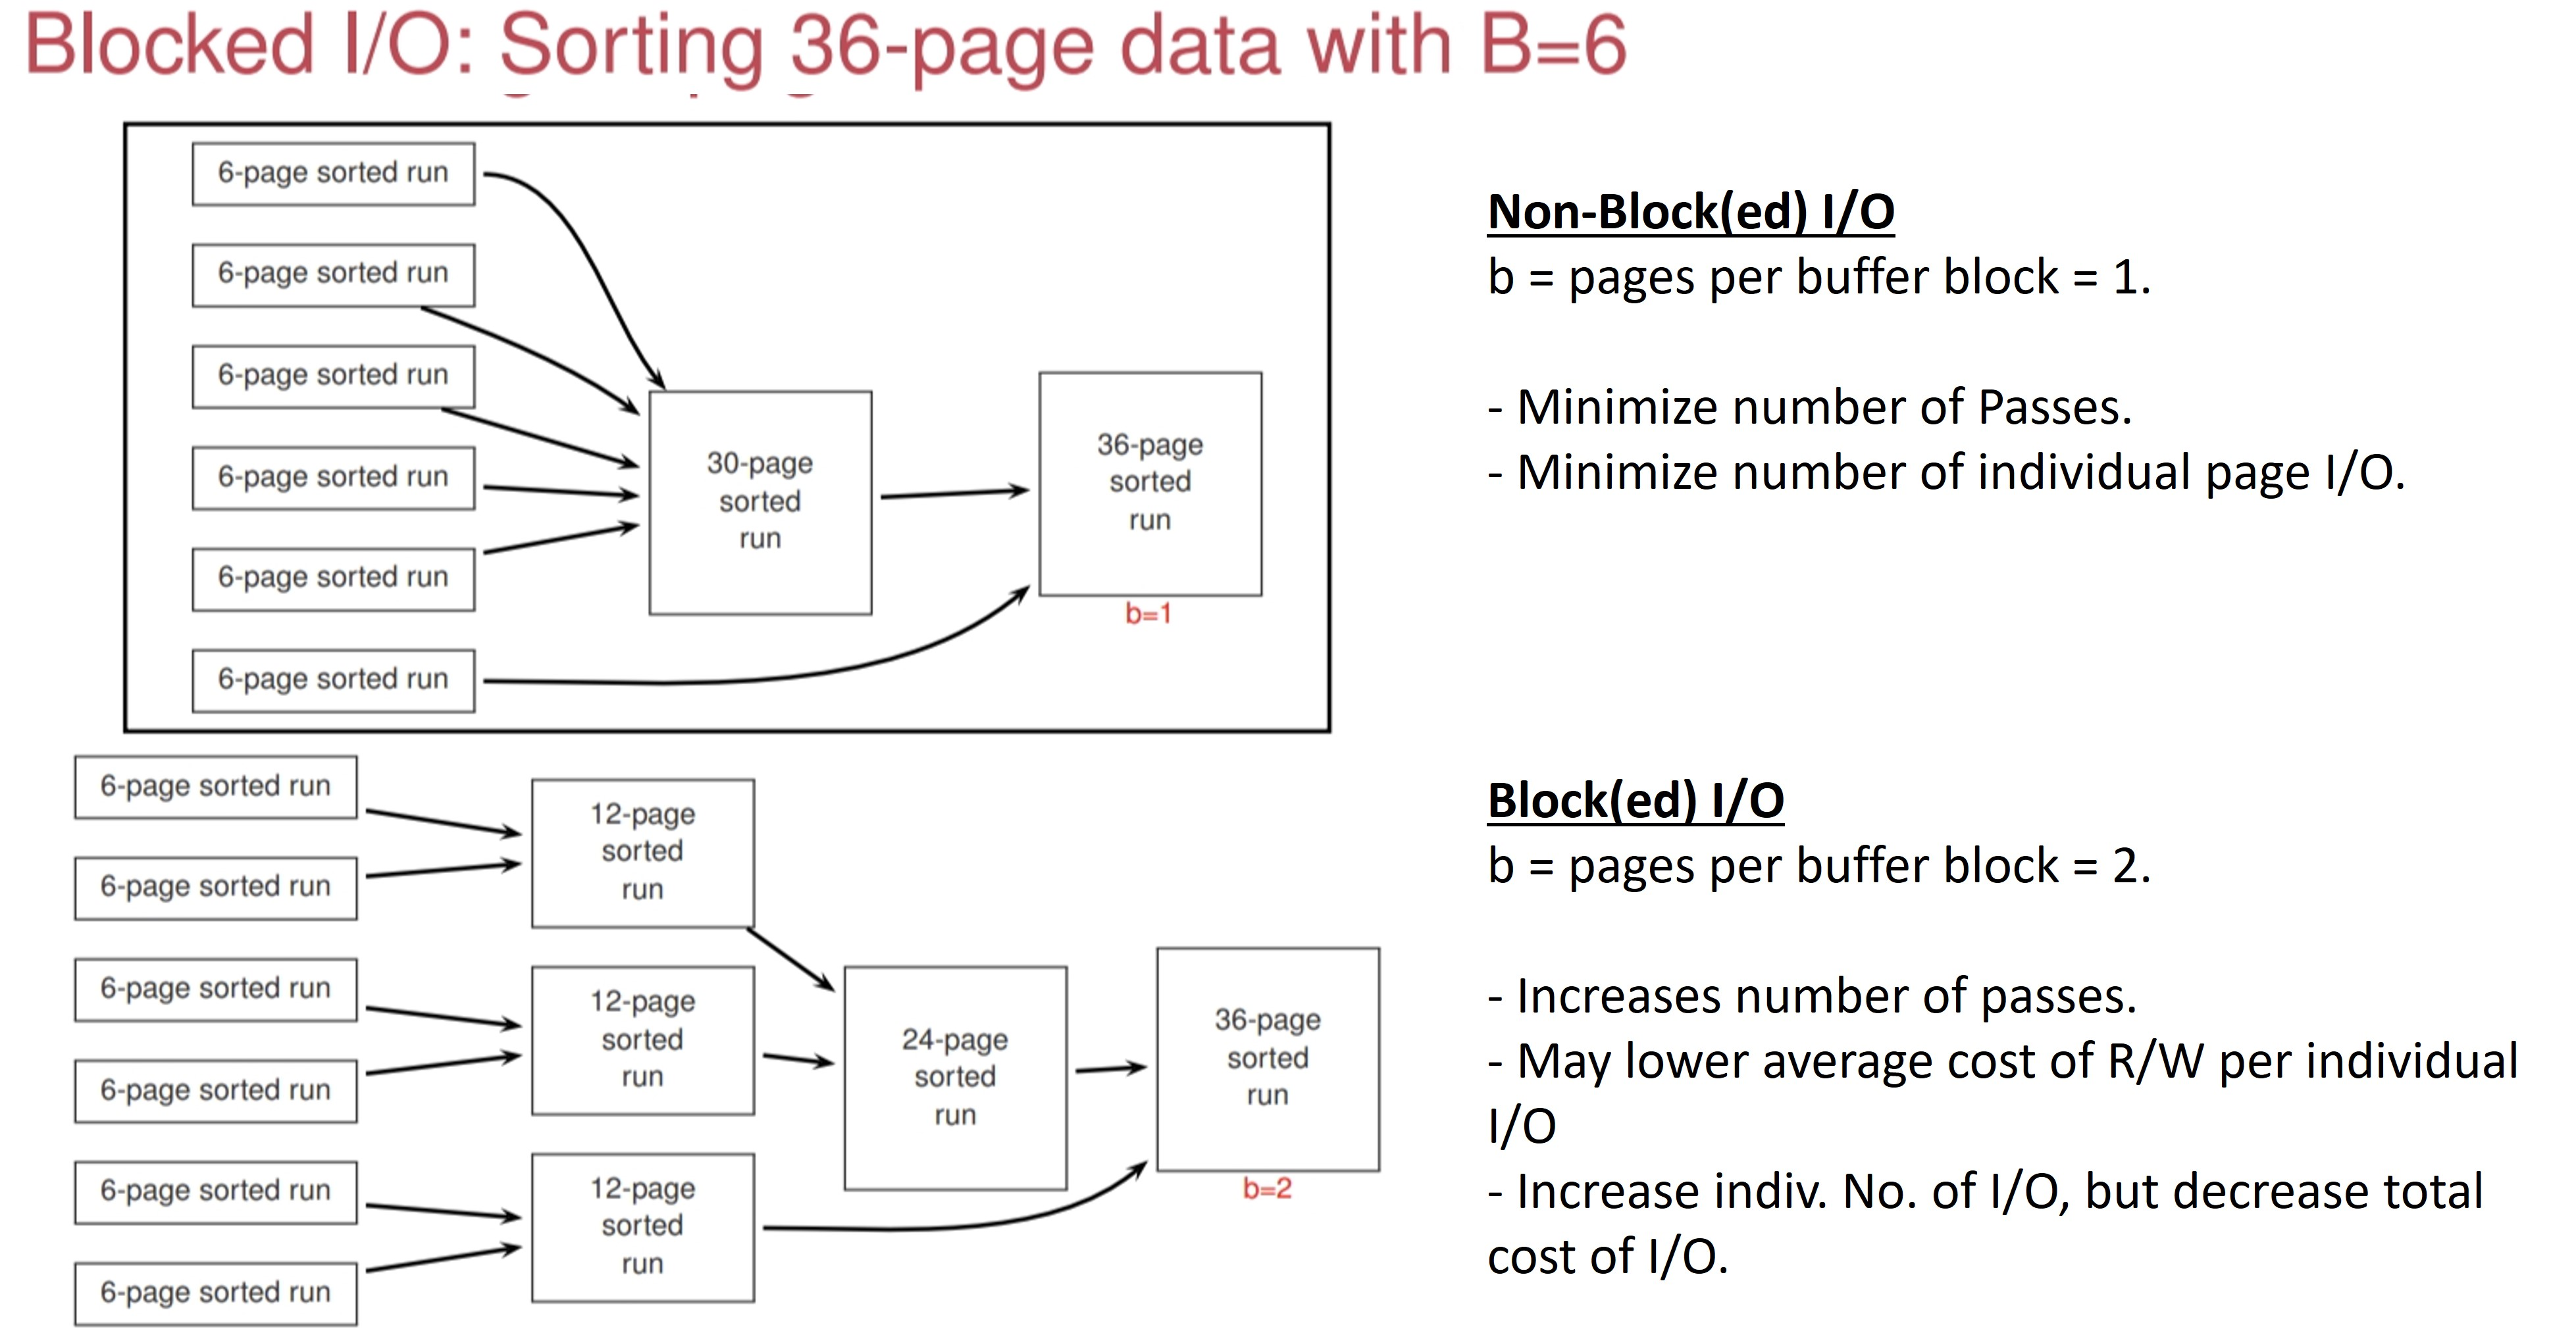
\includegraphics[width = 1\linewidth]{blockedIO2}}
\begin{itemize}
\item \textbf{Overall}: \\
- Larger buffer blocks, (lower average page I/O cost). \\
- But num. passes increase, num page I/O increase. 
\item \textbf{Decrease per-page I/O cost tradeoffs Increase No. of page I/Os.}
\end{itemize}

\columnbreak

\subsection{Sorting using $B^+$-trees}
\begin{itemize}
\item When table to be sorted has existing $B^+$-tree index on sorting attributes.
\begin{itemize}
\item Format 1: Sequentially scan leaf pages of $B^+$-tree.
\item Format 2/3:  Sequentially scan leaf pages of $B^+$-tree. For each leaf page visited, retrieve data records using RIDs.
\end{itemize}
\end{itemize}

\section{Selection $\sigma_p(R)$}
Select rows from Relation $R$ that satisfy selection predicate $p$
\begin{itemize}
\item \textbf{Index Matching}: Index \textbf{matches} selection predicate if index can be used to evaluate it. Consider Hash index, and B+ Tree index.
\end{itemize}

\subsection{Access Path}
\begin{itemize}
\item \textbf{Access path} refers to the given way of accessing data records/entries.
\begin{itemize}
\item \textbf{Table scan}: scan all data pages.
\item \textbf{Index scan}: scan all index pages.
\item \textbf{Index Intersection}: Combine results from multiple index scans (e.g. intersect, union).
\end{itemize}
\item Index scan/intersect follow by \textbf{RID lookups} to retrieve data records.
\end{itemize}

\subsubsection{Selectivity of Access Path}
\centerline{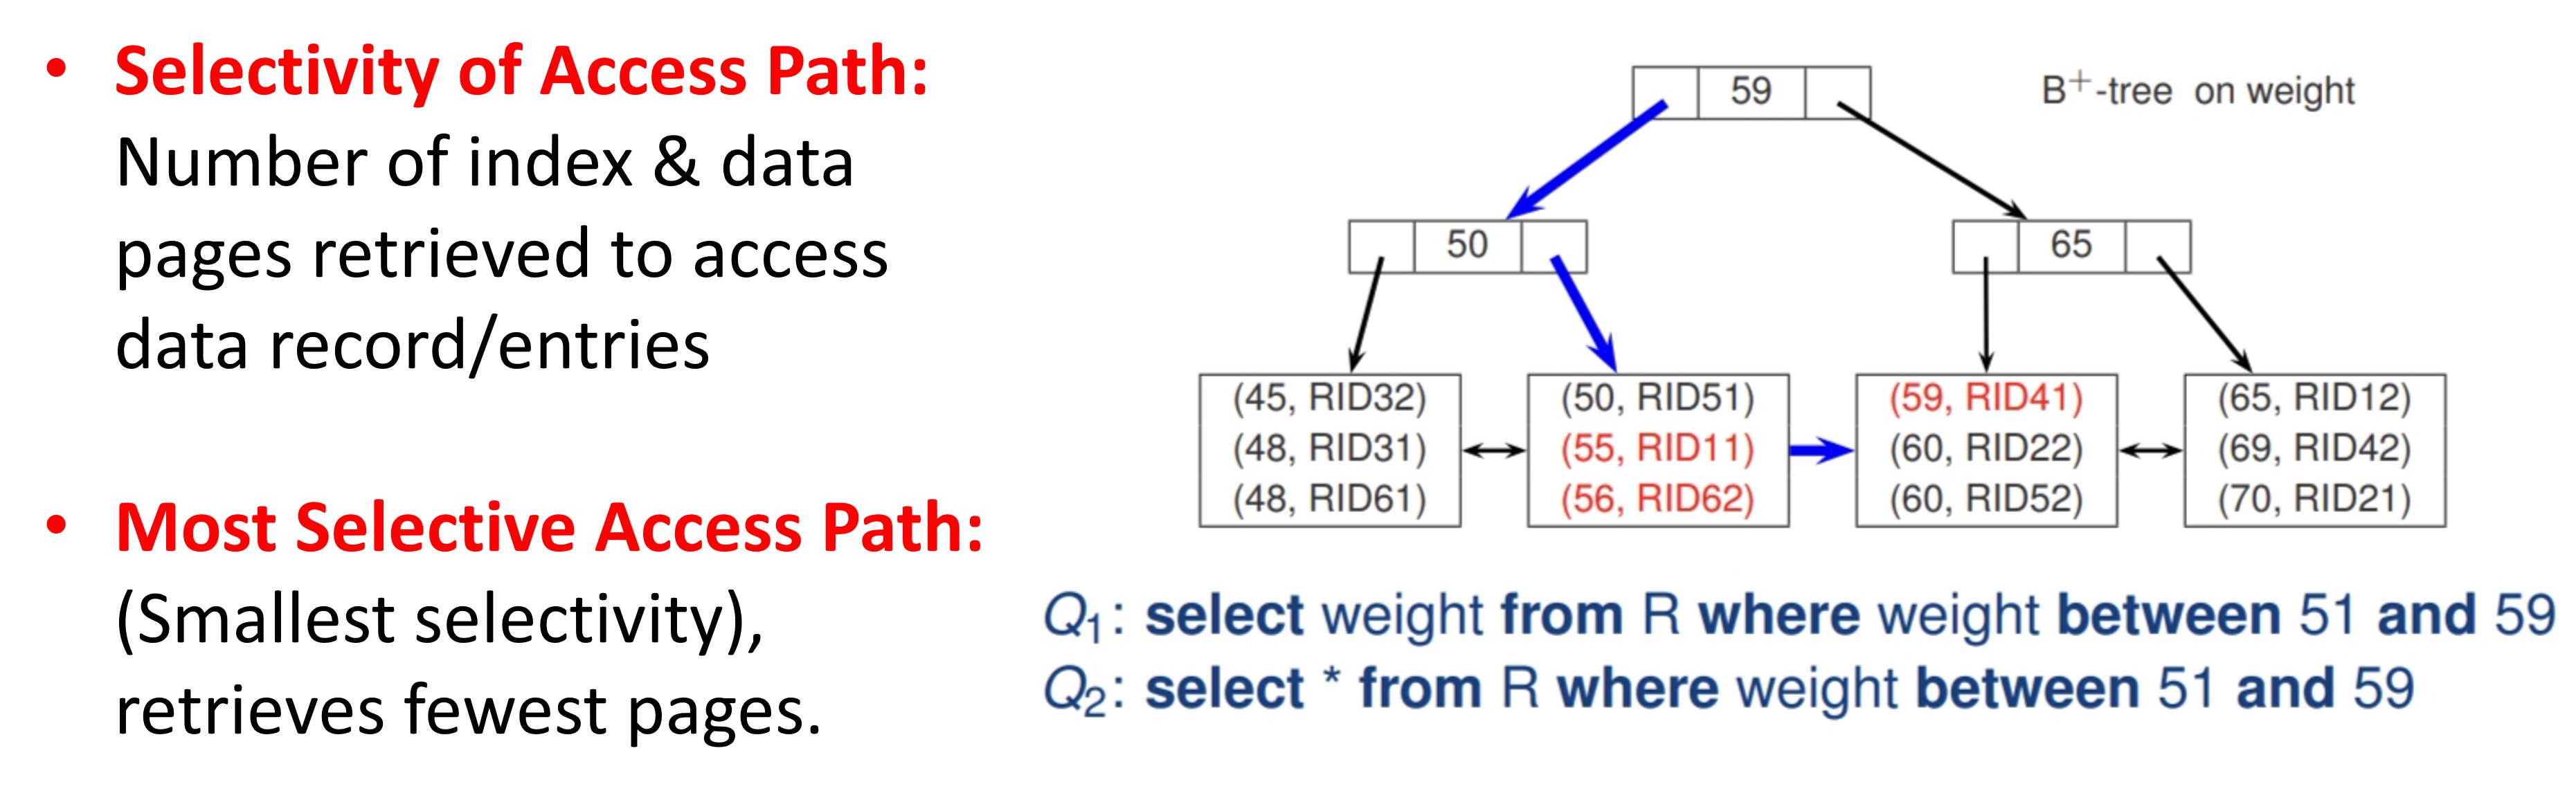
\includegraphics[width = 1\linewidth]{selectivity}}
\begin{itemize}
\item \textbf{Most Selective Access Path minimizes cost of data retrieval.}
\end{itemize}

\subsection{Covering Index}
\centerline{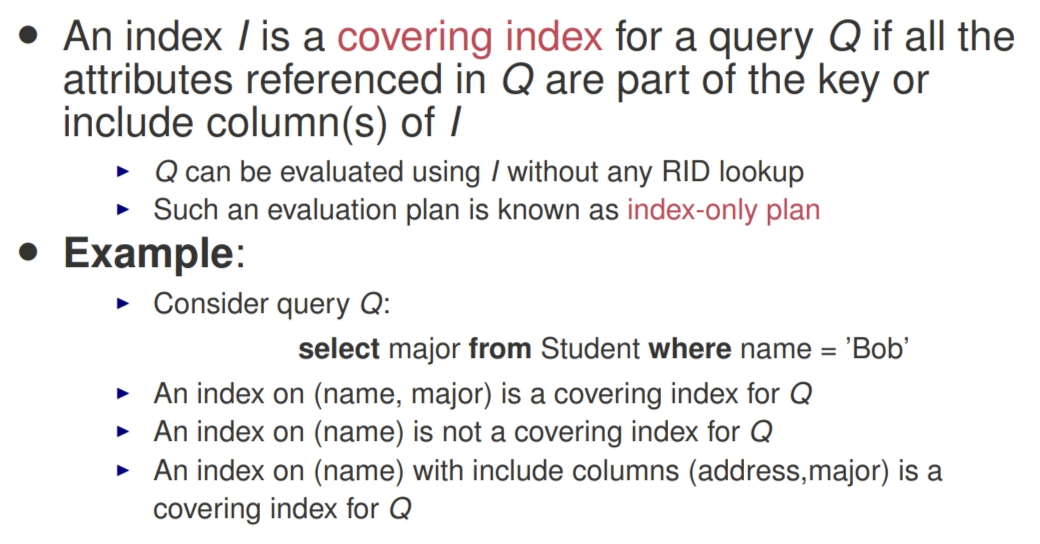
\includegraphics[width = 0.7\linewidth]{coveringIndex}}

\subsubsection{$B^+$-Tree: Include Columns (In Index)}
\centerline{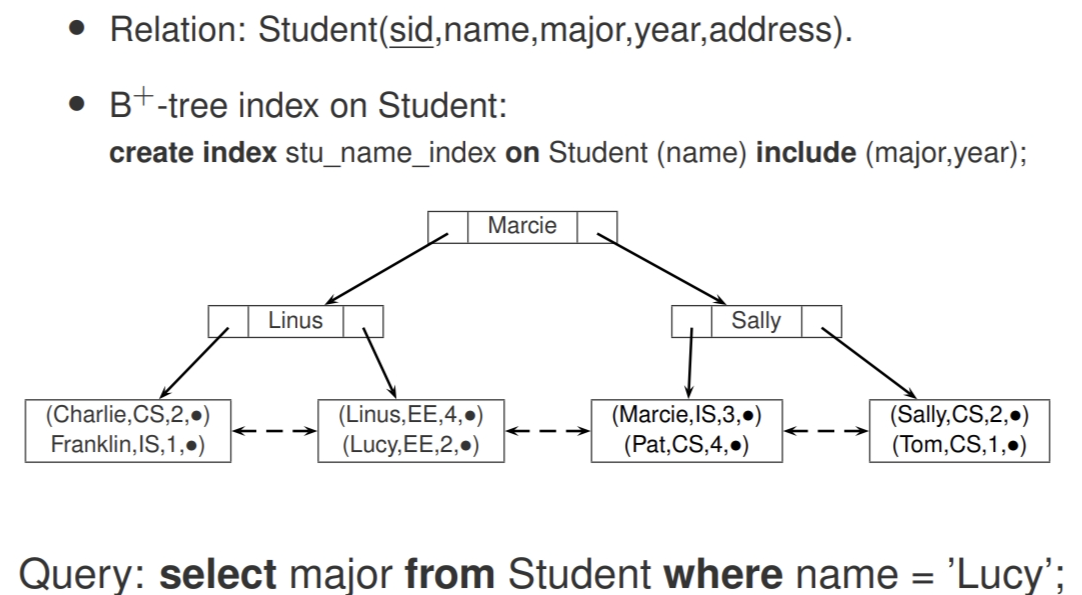
\includegraphics[width = 0.7\linewidth]{includeColumns}}

\subsection{$B^+$-Tree: Selection Evaluation}
\centerline{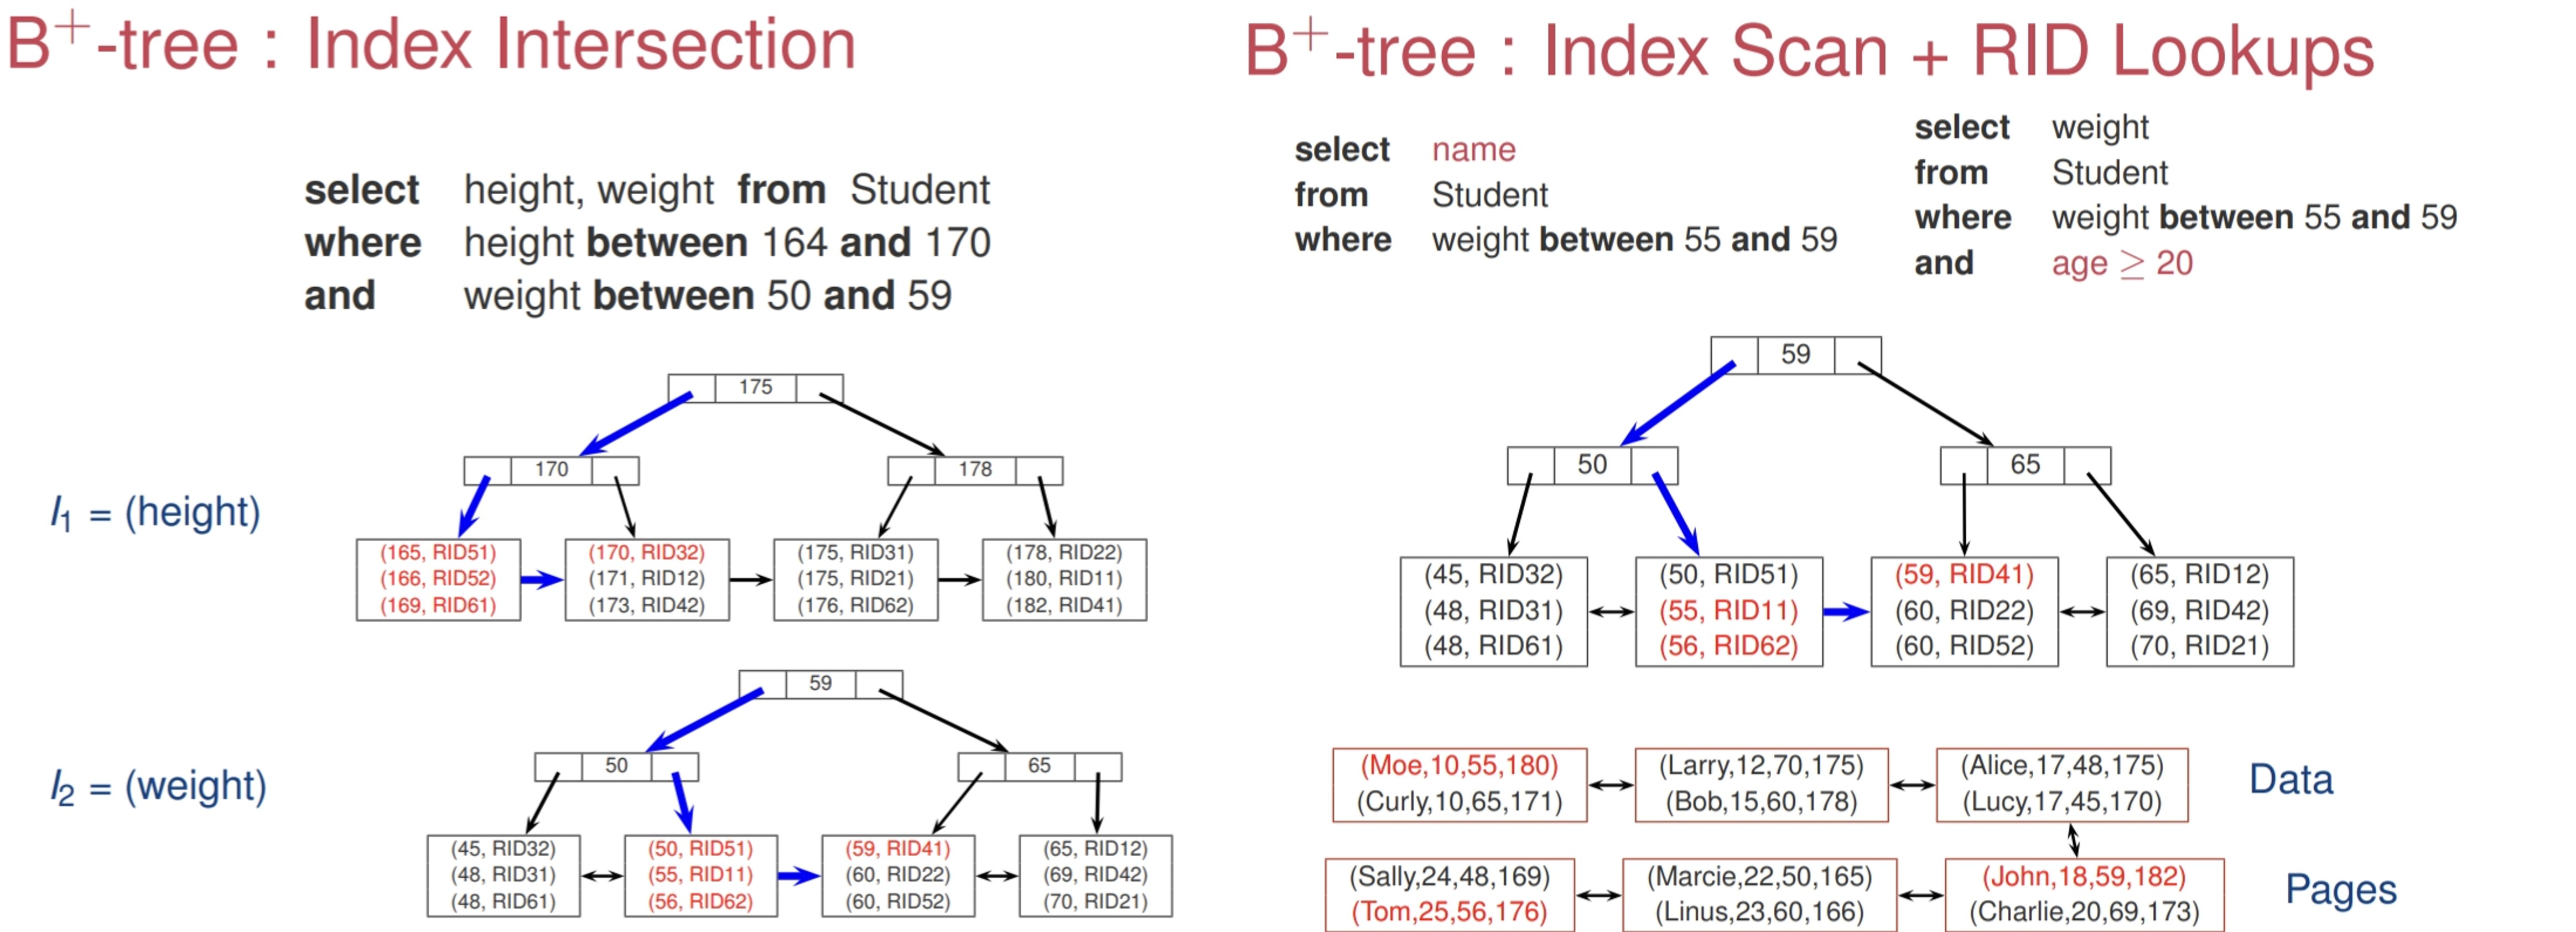
\includegraphics[width = 1\linewidth]{bTreeSelectionEvaluation}}

\subsection{CNF Predicates}
\begin{itemize}
\item \textbf{Selectivity of an access path} depends on primary conjuncts in selection condition (w.r.t. index involved.)
\item Each conjunct acts as filter on table, fraction of tuples satisfying given conjuct called reduction factor.
\end{itemize}

\centerline{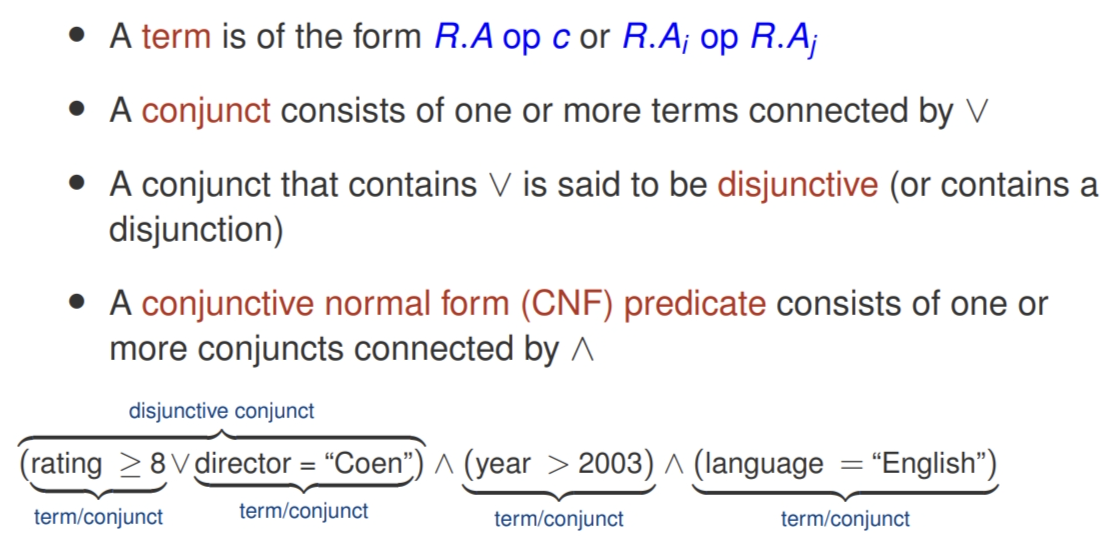
\includegraphics[width = 1\linewidth]{CNF}}
\begin{itemize}
\item \textbf{Non-equality Comparison Operators}: $<, \leq, >, \geq, <>$, between, in.
\end{itemize}

\subsection{Tree Index matching CNF Selection}
\begin{itemize}
\item Determines if Index is useful / appropriate, if index can be used to retrieve just the tuples that satisfy the condition.
\end{itemize}
\centerline{\includegraphics[width = 1\linewidth]{matchingPredicatesTree}}

\subsection{Hash Index matching CNF Selection}
\centerline{\includegraphics[width = 1\linewidth]{matchingPredicatesHash}}

\columnbreak

\subsection{Examples of Index matching CNF Selection}
\centerline{\includegraphics[width = 1\linewidth]{matchingPredicates}}
\medskip

\subsubsection{Primary and Covered Conjuncts}
\begin{itemize}
\item \textbf{Primary Conjuncts}: Subset of conjuncts in selection predicate $p$ that index $I$ \textbf{matches}.
\item In general, only subset of conjuncts of predicate matches index.
\item \textbf{Covered Conjunct}: Conjunct C in predicate $p$ covered if all attributes in $C$ appear in the key, or \textit{include column(s)} of index $I$.
\item Primary conjuncts subset of covered conjuncts.
\end{itemize}

\subsection{Cost of Evaluation of Selection Predicate $p$}
\centerline{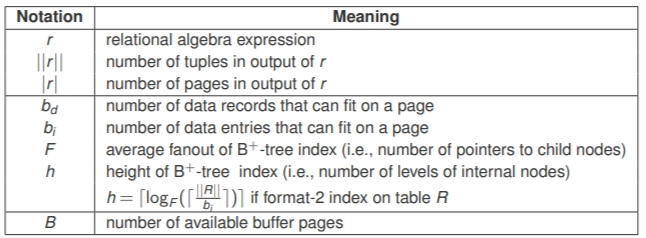
\includegraphics[width = 0.9\linewidth]{notation}}

\subsection{Cost of $B^+$-tree Index Evaluation of $p$}
\centerline{\includegraphics[width = 0.95\linewidth]{BTreeEvaluationCost}}
\centerline{\includegraphics[width = 0.95\linewidth]{BTreeEvaluationCostExample}}

\subsection{Cost of Hash Index Evaluation of $p$}
\centerline{\includegraphics[width = 0.95\linewidth]{hashEvaluationCost}}

\subsection{Evaluating Non-Disjunctive / Disjunctive Conjuncts}
\centerline{\includegraphics[width = 1\linewidth]{Disjunct}}
\begin{itemize}
\item \textbf{Possible strategies to evaluate Disjunctive / Non-Disjunctive predicates}
\item File scan, Use both (fetch RID, take Union), Use B+ tree etc.
\end{itemize}


\section{Clustered vs. Unclustered Index (B+Tree)}
\begin{itemize}
\item \textbf{Clustered Index}: Order of its data entries is the same or `close to' order of the data records (in pages).
\item Layman Terms: If clustered, if we do a file scan, records will be in order with respect to the attribute.
\item An index using Format 1 for data entries is a clustered index.
\item Logically, at most one clustered index for each relation.
\item \textbf{Implication}: Tutorial 3 Q4: When doing index scan with RID lookup, for clustered index, RID page I/O incurred will be the number of leaf pages.

\item \textbf{Unclustered Index}: Order of data entries not same as actual order of data records. To retrieve each tuple / entry, need to do separate RID lookup / page retrieval. 
\item \textbf{Implication}: Tutorial 3 Q4: When doing index scan with RID lookup, for unclustered index, RID page I/O incurred will be number of pages of tuples ($>$ no. of leaf pages.
\end{itemize}
\centerline{\includegraphics[width = 0.95\linewidth]{clusteredIndex}}

\section{Dense vs. Sparse Index (B+Tree)}
\begin{itemize}
\item \textbf{Dense index}: there is an index record for every search key value in the data.
\item The total number of records in the index table and main table are the same.
\item Gives quick access to records, effective for range searches as each key value has an entry, but takes more storage, and insertion and deletion higher overhead.
\item For \textit{unclustered index}, must be dense.

\item \textbf{Sparse index}: Some search key value has no have index record. (Main table index points records in specific gap (range of space where index resides in).
\item Uses less storage space, lessen effect of insert/delete on index maintenance operations. Time to locate data in index table more, and sparse index records need to be clustered.
\item For sparse index, records need to be clustered (in order).
\end{itemize}
\centerline{\includegraphics[width = 1\linewidth]{denseIndex}}
\medskip
\centerline{\includegraphics[width = 0.8\linewidth]{denseIndex2}}
\medskip
\centerline{\includegraphics[width = 0.8\linewidth]{clusteredIndex2}}

\vfill \null
\columnbreak

\section{PostgreSQL: Buffer Replacement Policy}
PostgreSQL: Open source relational database management system.

\begin{itemize}
\item \textbf{Port Number}: By default, server listens on port number 5432 for client connections.
\item PostgreSQL uses variant of Clock policy as default buffer replacement policy. 
\end{itemize}

\subsection{Overview of PostgreSQL}
\subsubsection{Shared-memory Data Structures}
\begin{itemize}
\item As multiple backend server processes may access database at same time, access to shared-memory structures (buffer pool) controlled to ensure consistent access and updates. Use \textbf{locks} (spin locks, light-weight locks) to control access.
\item \textbf{Locking Protocol}: Before accessing shared-memory structure, process acquire lock, upon completion of access, process release lock.
\end{itemize}

\subsubsection{Buffer Manager}
\begin{itemize}
\item Two main types of Buffers used: Shared Buffer, Local Buffer.
\item \textbf{Shared Buffer}: Used for holding page from globally accesible relation. 
\item \textbf{Local Buffer}: Usef for holding page from temporary relation locally accessible to specific process.
\end{itemize}

\subsubsection{Management of Shared Buffers}
\begin{itemize}
\item Initially, all shared buffers maintained in free list.
\item \textbf{Free list}: Buffer in free list if contents invalid. When new buffer needed, check if buffer available in free list, returned to satisfy buffer request.
\item If no available buffer, use \textbf{buffer replacement policy} to select victim buffer for eviction to make room for new request. (Use variant of Clock algorithm)

\item \textbf{Record Deleted/Modified}: Not immediately removed/changed. Multiple versions of record maintained to support \textbf{multiversion concurrency control}.
\item \textbf{Vacuuming Process}: Periodically, vacuuming process runs to remove obsolete versions of records that can be safely deleted from relations. If entire page of records removed, buffer holding page becomes invalid, returned to free list.
\item \textit{bgwriter}: background writer process that writes out dirty shared buffers to partly help speed up buffer replacement.
\end{itemize}

\subsubsection{PostgreSQL Buffer Pool}
\begin{itemize}
\item \textbf{Buffer Pool}: Implemented as array of disk blocks, index to each array entry referred to a \code{buffer_id}, each disk block location identified by buffer tag.
\item Pin count for each buffer frame known as reference count \code{refcount}.
\item Each buffer frame associated with a buffer descriptor, stores metadata about contents.
\item Given a buffer tag, hash-based buffer table is used to efficiently locate buffer id of buffer frame that stores the disk block (corresponding to given tag) if disk block resident in buffer pool.
\end{itemize}

\columnbreak

\subsection{Implementing LRU Buffer Replacement Policy}
\begin{itemize}
\item Simple approach to implement LRU Policy: \textbf{Stack LRU} Method.
\item Use doubly Linked List to link up buffer pages. Page closer to the front is more recently used, than page closer to tail of list.
\item Whenever buffer page referenced (``Used''), moved to front of list. 
\item When replacement page sought from list, \textbf{unpinned} buffer page closest to tail (LRU) selected for eviction.
\item \textbf{Whenever buffer accessed, position needs to be adjusted}:
\begin{enumerate}
\item If accessed page in buffer pool already, containing buffer needs to be moved to top of stack.
\item If accessed page not in buffer pool, \textbf{free buffer available} to hold page, selected buffer from free list needs to be inserted onto top of stack.
\item If accessed page not in buffer pool, \textbf{free list empty}, selected victim buffer moved from current stack position to top of the stack.
\item If buffer in buffer pool \textbf{returned to the free list}, buffer removed from stack.
\end{enumerate}
\end{itemize}

\subsection{Enhanced LRU (ELRU) Buffer Replacement Policy}
\begin{itemize}
\item A disadvantage of LRU is that a page that is accessed only once could evict a frequently accessed page from the buffer.
\item To address this limitation, ELRU, which is a variant of LRU, keeps track of additional page access information to manage the eviction of buffer pages in two separate groups.
\item In contrast to LRU which uses only the last access time of buffer pages, ELRU maintains the last two access times of buffer pages.
\end{itemize}

\subsubsection{Specifications of ELRU}
\begin{itemize}
\item Specifically, let $B = B_1 \cup B_2$ denote the set of unpinned buffer pages that can be selected for replacement.
\item $B_1$  is the set of buffer pages that have been accessed only once.
\item $B_2$  is the set of buffer pages that have been accessed at least twice. 
\item The ELRU policy selects a replacement page from $B$ for replacement as follows. If $B_1$ is non-empty, ELRU selects the least recently accessed page in $B_1$
 as the replacement page; i.e., ELRU applies the conventional LRU policy to select the replacement page from $B_1$. Otherwise, if $B_1$ is empty, ELRU selects the page in $B_2$
 with the smallest second-last access time as the replacement page.
\end{itemize}


\null \null \null \null
\columnbreak

\subsection{PostgreSQL:  Normal Buffer Replacement Strategy (Clock-Sweep)}
\begin{itemize}
\item \textbf{PostgreSQL standard Buffer Replacement Strategy}
\item There is a "free list" of buffers that are prime candidates for replacement.
In particular, buffers that are completely free (contain no valid page) are
always in this list.  We could also throw buffers into this list if we
consider their pages unlikely to be needed soon; however, the current
algorithm never does that.  The list is singly-linked using fields in the
buffer headers; we maintain head and tail pointers in global variables.
(Note: although the list links are in the buffer headers, they are
considered to be protected by the buffer\_strategy\_lock, not the buffer-header
spinlocks.)  
\item To choose a victim buffer to recycle when there are no free
buffers available, we use a simple clock-sweep algorithm, which avoids the
need to take system-wide locks during common operations.  It works like
this:
\item Each buffer header contains a usage counter, which is incremented (up to a
small limit value) whenever the buffer is pinned.  (This requires only the
buffer header spinlock, which would have to be taken anyway to increment the
buffer reference count, so it's nearly free.)
\item The "clock hand" is a buffer index, nextVictimBuffer, that moves circularly
through all the available buffers.  nextVictimBuffer is protected by the
buffer\_strategy\_lock.
\end{itemize}

\subsubsection{Clock-Sweep Buffer Replacement Algorithm}
\begin{itemize}
\item The \textbf{algorithm} for a process that needs to obtain a victim buffer is:
\begin{enumerate}
\item Obtain buffer\_strategy\_lock.
\item If buffer free list is nonempty, remove its head buffer.  Release
buffer\_strategy\_lock.  If the buffer is pinned or has a nonzero usage count,
it cannot be used; ignore it go back to step 1.  Otherwise, pin the buffer,
and return it.
\item Otherwise, the buffer free list is empty.  Select the buffer pointed to by
nextVictimBuffer, and circularly advance nextVictimBuffer for next time.
Release buffer\_strategy\_lock.
\item If the selected buffer is pinned or has a nonzero usage count, it cannot
be used.  Decrement its usage count (if nonzero), reacquire
buffer\_strategy\_lock, and return to step 3 to examine the next buffer.
\item Pin the selected buffer, and return.
\end{enumerate}
\item (Note that if the selected buffer is dirty, we will have to write it out
before we can recycle it; if someone else pins the buffer meanwhile we will
have to give up and try another buffer.  This however is not a concern
of the basic select-a-victim-buffer algorithm.)
\end{itemize}



\null \null \null \null
\columnbreak

\section{5. Query Evaluation: Projection \& Join}

\section{5.1 Projection: $\pi_{A1,...,Am}(R)$}
\begin{itemize}
\item $\pi_{L}(R)$ projects columns given by list L from relation R.
\item $\pi^*_{L}(R)$ same as $\pi_{L}(R)$ but preserves duplicates.
\item Example: \code{select distinct age from R}
\end{itemize}

\subsection{Projection Operation  $\pi_{A1,...,Am}(R)$}
\begin{itemize}
\item \textbf{Projection involves two tasks}: 
\begin{enumerate}
\item Remove unwanted attributes. (from tuples)
\item Eliminate any duplicate tuples produced.
\end{enumerate}
\item \textbf{Two approaches to Project}:
\begin{enumerate}
\item Projection based on \textbf{sorting}.
\item Projection based on \textbf{hashing}.
\end{enumerate}
\end{itemize}

\subsection{5.1.1 Sort-based Approach}

\subsubsection{Simple Sort-based Approach}
\begin{itemize}
\item Treat each step as a black box, push tuples through pipeline to sort.
\end{itemize}
\centerline{\includegraphics[width = 0.9\linewidth]{naivesort}}
\medskip
\centerline{\includegraphics[width = 0.9\linewidth]{naivesortcost}}

\subsubsection{Optimized Sort-based Approach}
\begin{itemize}
\item By opening black box and examining the sort algorithm (external merge sort), we can optimize the sort-based approach.
\end{itemize}
\centerline{\includegraphics[width = 0.75\linewidth]{optimizedsort}}

\subsection{5.1.2 Hash-based Approach}
\begin{itemize}
\item For  , we build a \textbf{main-memory hash table} T to detect and remove duplicates.
\item Cost = $|R|$ if T fits in main memory.
\item \textbf{Two Phases}: Partitioning phase and Duplicate Elimination phase.
\end{itemize}
\centerline{\includegraphics[width = 1\linewidth]{hashBasedPhases}}
\smallskip

\subsubsection{Overview of Hash-based Approach}
\centerline{\includegraphics[width = 1\linewidth]{hashBased}}
\smallskip

\centerline{\includegraphics[width = 1\linewidth]{hashBasedPhases2}}

\subsubsection{Hash-based Approach Partition Overflow}
\begin{itemize}
\item \textbf{Partition Overflow Problem}: When hash table for $\pi^*_{L}(R)$ (Partitioned table) is larger than available memory buffers.
\item Recursively apply hash-based partitioning to the overflowed partition.
\end{itemize}
\centerline{\includegraphics[width = 1\linewidth]{overflow}}

\subsubsection{Notation}
\centerline{\includegraphics[width = 0.9\linewidth]{notation}}


\subsubsection{Illustration of Partitioning, Duplicate Elimination Phase}
\centerline{\includegraphics[width = 1\linewidth]{partitioningDuplicateEliminationPhase}}

\subsubsection{Analysis of Hash-based Approach}
\begin{itemize}
\item Approach is effective if \textbf{B is large relative to $|R|$.}
\end{itemize}
\centerline{\includegraphics[width = 0.9\linewidth]{hashAnalysis}}


\subsection{Sort-based vs. Hash-based Analysis}
\centerline{\includegraphics[width = 0.9\linewidth]{sortvsHash}}

\subsection{5.1.3 Projection Operation: using Indexes}
\begin{itemize}
\item If there is an index whose search key ($+$ include columns) contains all wanted attributes, \textbf{replace table scan with index scan}.
\item If index ordered (B$+$-tree), search key includes wanted attributes as prefix, scan data entries in order, compare adjacent duplicate data entries.
\item E.g. B$+$-tree index on $R$ with key (A, B) to evaluate query $\pi_{A}(R)$.
\end{itemize}


\section{5.2 Join: $R_{\bowtie_\theta}S$}
\begin{itemize}
\item Join is where there is match between values of specified columns. 
\item Two-table joins, multiple-table joins, self-joins etc.
\item Example: \code{SELECT * FROM customer c, orders o WHERE c.name = o.name;}
\end{itemize}
\centerline{\includegraphics[width = 1\linewidth]{joinOperation}}

\subsection{Join Algorithms}
\begin{itemize}
\item \textbf{Iteration-Based}: Block nested loop.
\item \textbf{Index-Based}: Index nested loop.
\item \textbf{Partition-Based}: Sort-merge join, hash join.
\end{itemize}

\subsubsection{Join Algorithms Analysis}
\begin{itemize}
\item \textbf{Factors to Consider}: 
\item \textit{Type of join predicates} (equality predicates e.g. $R.A_i = S.B_j$), (inequality predicates e.g. $R.A_i < S.B_j$)
\item \textit{Size of join operands}
\item Available \textit{buffer space}, available \textit{access methods}.
\item Given a join $R_{\bowtie_\theta}S$, R is \textbf{outer relation}, S is \textbf{inner relation}
\end{itemize}

\subsection{Tuple/Page-based Nested Loop Join (Naive)}
\begin{itemize}
\item Simplest join algo is \textbf{tuple-at-a-time} nested loop evaluation. We scan outer relation R, and for each tuple in R, scan inner relation S.
\item Simple refinement is \textbf{join page-at-a-time}. For each page of R, retrieve each page of S, and write out matching tuples.
\item Importance of page-orientated operations for minimizing disk I/O.
\item \textbf{Observation}: Choose outer relation R to be smaller of two relations.
\end{itemize}
\smallskip
\centerline{\includegraphics[width = 1\linewidth]{nestedJoinLoop}}

\columnbreak

\subsection{5.2.1 Block Nested Loop Join}
\begin{itemize}
\item Simple nested loops join algo does not effectively utilize buffer pages.
\item If enough memory, read whole of R (smaller relation), use one of extra buffer page to scan larger relation S. Last buffer page used as output buffer. Each relation scanned just once, optimal!
\item \textbf{Generalization}: Break relation R into \textit{blocks} that can fit into available buffer pages, and scan all of S for each block of R. 
\item $R$ is \textbf{outer relation}, as it is scanned only once. $S$ is \textbf{inner relation}, scanned multiple times.
\end{itemize}
\centerline{\includegraphics[width = 1\linewidth]{blockedNestedLoop}}

\subsection{5.2.2 Index Nested Loop Join}
\begin{itemize}
\item If exists index on one of the relations on the join attribute(s), take advantage by making \textbf{indexed relation to be inner relation (S)}.
\item For each tuple in R, use index to retrieve matching tuples of S.
\item Cost of scanning R is M, and cost of retrieving matching S tuples depends on kind of index and number of matching tuples.
\end{itemize}
\centerline{\includegraphics[width = 1\linewidth]{indexNestedLoop}}

\columnbreak

\subsection{5.2.3 Sort-Merge Join}
\begin{itemize}
\item Basic idea: Sort both relations on join attribute and look for qualifying tuples by essentially merging the two relations.
\item Exploit partitioning, compare R tuples with only S tuples in same partition (rather than all S tuples), avoid enumeration of cross-product of R \& S. (Works only for equality join conditions.)
\end{itemize}
\centerline{\includegraphics[width = 1\linewidth]{sortMergeJoin}}
\centerline{\includegraphics[width = 1\linewidth]{sortMergeJoin2}}
\centerline{\includegraphics[width = 1\linewidth]{sortMergeJoin3}}

\columnbreak

\subsection{5.2.4 Hash Join}
\begin{itemize}
\item Hash join algorithm, like sort-merge join, identifies partitions in R \& S in partitioning phase, and compares tuples in corresponding partitions.
\item \textbf{Idea}: Unlike sort-merge join, use \textbf{hashing to identify partitions} over sorting. Hash both relations on join attribute using \textbf{same hash function $h$}. 
\item Partitioning (building) phase of hash join similar to partitioning in hash-based projection.
\end{itemize}


\subsection{Grace Hash Join}
\begin{itemize}
\item University of Tokyo, (1981), GRACE parallel relational database machine. Enables handling of large data stream quite efficiently in parallel.
\end{itemize}
\centerline{\includegraphics[width = 1\linewidth]{hashJoin}}
\centerline{\includegraphics[width = 1\linewidth]{hashJoin2}}


\section{6. Query Evaluation \& Optimization}
\section{6.1 Set Operations}
Set operations include \textbf{cross product} ($R \times S$), \textbf{intersection} ($R \cap S$), \textbf{union} ($R \cup S$), \textbf{difference} ($R - S$).
\begin{itemize}
\item Note that \textbf{intersection \& cross-product} are just special cases of join! (with equality on all fields as join condition for intersection, and with no join condition for cross-product).
\item \textbf{Union}: Main point to addresss is elimination of duplicates.
\item \textbf{Difference}: Variation of technique for duplicate elimination. Both can use sorting-based approach or hashing-based approach.
\end{itemize}
\centerline{\includegraphics[width = 1\linewidth]{sortHash}}

\section{6.2 Aggregation Operations}

\subsubsection{Simple Aggregation}
\begin{itemize}
\item E.g. \code{select count(*) from Movies}
\item \textbf{Aggregate Operators}: SUM, COUNT, AVG, MIN, MAX
\item \textbf{Algorithm}: Maintain some running information while scanning table.
\end{itemize}

\subsubsection{Group-by Aggregation}
\begin{itemize}
\item \code{select year, count(*) from Movies group by year}
\item \textbf{Sorting Approach}: Sort relation on grouping attribute(s), scan sorted relation to compute aggregate for each group.
\item \textbf{Hashing Approach}: Scan relation to build a hash table on grouping attribute(s), For each group, maintain (grouping-value, running-information).
\item \textbf{Using Index}: If there is covering index for query, avoid table scan. Aggregation operation can be computed from index's data entries instead of data records.
\item \textbf{Ordered scan using index}: For group-by aggregation, if set of group-by attributes forms a prefix of a B
+-tree index’s search key, the data entries (and data records if necessary) for each group can beretrieved without an explicit sorting.,
\end{itemize}

\columnbreak

\section{6.3 Query Evaluation}

\subsection{6.3.1 Query Evaluation Approaches}
\subsubsection{Materialized Evaluation}
\begin{itemize}
\item An operator is evaluated only when each of its operands has been completely
evaluated or materialized.
\item Intermediate results are materialized to disk
\end{itemize}

\subsubsection{Pipelined Evaluation}
\begin{itemize}
\item The output produced by a operator is passed directly to its parent operator.
\item Execution of operators is interleaved. Top-down, demand-drive approach.
\item An operator O is a \textbf{blocking operator} if O may not be able to produce any output until it has received all the input tuples from its child operator(s). Examples of blocking operator: external merge sort, sort-merge join, Grace hash join.
\item \textbf{Iterator Interface} for operator evaluation. "open, getNext, close" functions to initialize state of iterator, generate next output tuple and deallocate state information.
\item For examples of Iterator on Hash-based Projection, Nested Loop Join, Table Scan, see slides.
\end{itemize}

\subsubsection{Pipelined Evaluation with Partial Materialization}
Also possible to have a mix of both approaches.

\section{6.4 Query Processing}
\centerline{\includegraphics[width = 1\linewidth]{queryProcessing2}}

\subsection{Query Plans}
SQL Query $Q$ $\rightarrow$ Logical Plan for $Q$ $\rightarrow$ Physical Plan for $Q$. 
\centerline{\includegraphics[width = 1\linewidth]{QueryPlans}}

\columnbreak

\subsubsection{Logical Query Plans}
\begin{itemize}
\item A query generally has many equivalent \textit{logical query plans}.
\item E.g. for join, the number of logical query plans grows exponentially.
\end{itemize}
\centerline{\includegraphics[width = 1\linewidth]{QueryPlansLogical}}

\subsubsection{Physical Query Plans}
\begin{itemize}
\item Subsequently, each logical plan can be implemented by many physical query plans.
\end{itemize}
\centerline{\includegraphics[width = 1\linewidth]{QueryPlansPhysical}}

\subsubsection{Note: Join Plan Notation}
\centerline{\includegraphics[width = 1\linewidth]{joinPlanNotation}}

\section{6.5 Query Optimization}
The process of finding a good query evaluation plan is called query optimization. Optimizing a relational algebra expression involves (three) basic steps: 
\begin{enumerate}
\item \textbf{Search Space}: What is space (subset) of query plans being considered? (Since number of possible plans too large).
\item \textbf{Plan Enumeration}:	How to enumerate space of query plans. 
\item \textbf{Cost Model}:	Estimate cost of each enumerated plan, choose plan with lowest estimated cost.
\end{enumerate}
SQL queries optimized by decomposing into blocks, optimize single block at a time. A query block can be expressed as a \textbf{relational algebra expression}.

\subsection{Relational Algebra Equivalence Rules}
\centerline{\includegraphics[width = 1\linewidth]{equivalence}}
\begin{itemize}
\item Using equivalence, we can find equivalent logical query plans.
\item Generally, we want to push down selection, projection operations to reduce size of table for subsequent joining.
\end{itemize}

\subsection{Types of Query Plan Trees}
\begin{itemize}
\item \textbf{Linear}: Query plan is linear if at least one operand for each join operation is a base relation; otherwise, the plan is \textbf{bushy}.
\item A linear query plan is \textbf{left-deep} if every right join operand is a base relation, and \textbf{right-deep} if every left join operand is a base relation.
\end{itemize}
\centerline{\includegraphics[width = 1\linewidth]{queryPlanTrees}}

\subsection{6.5.1 Search Space (Pruning)}
Consider search space for simple two join operations: (12. Growth of search space is exponential!)
\centerline{\includegraphics[width = 0.8\linewidth]{queryPlanSearchSpace}}
\begin{itemize}
\item Not all algebraically equivalent plans considered, make cost of optimization prohibitively expensive.
\item \textbf{Use heuristics to prune search space}: (System R Optimizer) Enumerates only left-deep query plans, avoids cross-product query plans (only join with condition), Considers early selections \& projections.
\end{itemize}


\subsection{6.5.2 Query Plan Enumeration}
Dynamic programming (using solution of subset to solve superset problem).

\subsubsection{Straightforward DP formulation}
For each relation, consider best access plan. Then, for each subset of relations, consider best plan to join.
\centerline{\includegraphics[width = 0.9\linewidth]{dp}}

\subsubsection{Enhanced dynamic programming approach (System R Optimizer)}
Consider \textbf{sort order} of query plan's output. Also use heurisitics to prune search space.
\begin{itemize}
\item Maintains optPlan($S_i$, $o_i$i) instead of optPlan($S_i$).
\item $o_i$ captures the sort order of output produced by query plan wrt $S_i$, null if output is unordered or a sequence of attributes.
\item optPlan($S_i$, $o_i$i) = cheapest query plan for relation with output ordered by if not null
\end{itemize}
\centerline{\includegraphics[width = 0.9\linewidth]{systemR}}

\vfill \null
\columnbreak

\subsection{6.5.3 Cost Estimation of Query Plans}
Cost estimation involves the following:
\begin{enumerate}
\item What is the \textbf{evaluation cost} of each operation? Cost model depends on: size of input operands, available buffer pages,
available indexes, etc.
\item What is the \textbf{output size} of each operation?
\end{enumerate}
Use a \textbf{cost model} for each operator's algorithms. 

\subsubsection{Estimation Assumptions}
\begin{enumerate}
\item \textbf{Uniformity assumption}: uniform distribution of attribute values
\item \textbf{Independence assumption}: independent distribution of values in different attributes
\item \textbf{Inclusion assumption}: For Join R(R.A=S.B)S, if no. tuples in A $\leq$ B, consider $\pi_A(R) \subset \pi_B(R)$.
\end{enumerate}

\textbf{Database Statistics}: Relation cardinality (no. of tuples), no. of distinct values / highest / lowest / frequent values in each column, column group statistics, histograms etc.

\subsection{Size Estimation}
For selection operations across joins, to estimate $||q||$, each predicate term potentially filters out some tuples.
\begin{itemize}
\item \textbf{Reduction factor}: denoted $rf(t_i)$, is fraction of tuples in input relation that satisfy $t_i$.
\item \textbf{Reduction factor} also known as \textbf{Selectivity Factor}.
\end{itemize}
\centerline{\includegraphics[width = 1\linewidth]{sizeEstimation}}

\subsection{A. Selectivity Factor Estimation (within Relation)}
\begin{itemize}
\item \textbf{Simple Uniformity Assumption}: Using number of unique tuple values, find rf: \\
e.g. $||R|| = 45$, $||\pi_A(R)|| = 15$, $rf(A=c) \approx \frac{1}{||\pi_A(R)||} = \frac{1}{15}$
\end{itemize}
\centerline{\includegraphics[width = 1\linewidth]{sizeEstimationUA}}
\smallskip
\centerline{\includegraphics[width = 1\linewidth]{sizeEstimationUA2}}

\vfill \null
\columnbreak

\subsection{B. Join Selectivity (inter-Relation selectivity)}
\begin{itemize}
\item \textbf{Join selectivity factor}: Selectivity factor for join predicates
\item \textbf{Inclusion asumption}: Assume every (smaller) relation tuple joins with some (larger) relation tuple.
\end{itemize}
\centerline{\includegraphics[width = 1\linewidth]{joinSelectivity}}
\smallskip
\centerline{\includegraphics[width = 1\linewidth]{joinSelectivity2}}

\bigskip

\subsection{Estimation using Histograms}
\begin{itemize}
\item \textbf{Histogram}: stat. info maintained by DBMS to estimate data distribution.
\item \textbf{Main idea using histogram}: Partition attribute’s domain into sub-ranges called buckets, assume value distribution within each bucket is uniform.
\item \textbf{Equiwidth Histograms}: Each bucket has (almost) equal number of values
\item \textbf{Equidepth Histograms}: Each bucket has (almost) equal number of tuples, sub-ranges of adjacent buckets might overlap.
\item \textbf{MCV: Most Common Values}: Separately keep track of the frequencies of the top-k most common
values and exclude MCV from histogram’s buckets.
\item \textbf{Accuracy of histograms}: Equiwidth $<$ Equidepth $<$ w. MCV excluded.
\end{itemize}

\subsection{Type of Histograms \& Estimation Accuracy}
\centerline{\includegraphics[width = 0.9\linewidth]{equiwidthHistogram}}
\smallskip
\centerline{\includegraphics[width = 0.9\linewidth]{equidepthHistogram}}
\smallskip
\centerline{\includegraphics[width = 1\linewidth]{histogram1}}
\smallskip
\centerline{\includegraphics[width = 1\linewidth]{histogram2}}

\columnbreak

\section{7. Transaction Management}

\section{7.1 Transactions}
A transaction is an abstraction representing a logical unit of work. Ensure 4 properties of Xacts / Txn. (\textbf{ACID}). \\
\textbf{Concurrency control manager} component ensures isolate, \textbf{recovery manager component} ensures durability.

\begin{itemize}
\item \textbf{Atomicity}: Either all or none of the actions in Xact happen.
\item \textbf{Consistency}: If each Xact is consistent, DB starts consistent, ends up consistent.
\item \textbf{Isolation}: Execution of one Xact is isolated from other Xacts.
\item \textbf{Durability}: If a Xact commits, its effects persist.
\end{itemize}

\subsubsection{Notation}
\begin{itemize}
\item \textbf{Transaction Schedule}: a list of actions from a set of Xacts, where
the order of the actions within each Xact is preserved.
\item \textbf{Serial Schedule}: Actions of Xacts are not interleaved.
\item \textbf{Read From}: $T_j$ reads object $O$ from $T_i$ in schedule if last write action on $O$ is by $I$, and $J$ reads after.
\item \textbf{Final Write}: $T_i$ performs final write on $O$ in a schedule
S if it does the last write action on $O$.
\item \textbf{Correctness of Interleaved Xact Executions}: Correct if “equivalent” to some serial schedule over the same set of Xacts.
\end{itemize}

\subsection{View Equivalent / Serializable}
\textbf{View Equivalent}: Two schedules over same set of Xacts are view equivalent if they have \textbf{same read froms} and the \textbf{same final write}. \\
\textbf{View Serializable}: A schedule is a \textbf{view serializable schedule (VSS)} if it is view equivalent to some serial schedule over the same set of Xacts. 
\\
\textbf{Testing for View Serializability}: Given a schedule S, construct a directed graph (denoted by VSG(S)) to capture the read-from and final-write relations among the transactions in S. If VSG(S) is cyclic, then S is not VSS. If acyclic, it is VSS iff there exists serial schedule produced from topological ordering of VSG(S) that is view equivalent to S.

\subsection{Conflicting Actions}
\textbf{Conflict}: Two actions on same object conflict if at least 1 write, different Xacts. (E.g. W + R, W + W, R + W).

\subsubsection{Anomalies with Interleaved Xact Executions}
\begin{itemize}
\item \textbf{Dirty Read Problem (WR Conflict)}: $T_2$ reads object produced by uncomitted Xact (which then aborts).
\item \textbf{Unrepeatable Read Problem (RW Conflict)}: $T_2$ updates object, reading yields different values before and after while $T_1$ in progress.
\item \textbf{Lost Update Problem (WW Conflict)}: $T_2$ overwrites value of object while $T_1$ still in progress.
\item \textbf{Phantom Read}: Re-executing query on search condition gives different results (bc new added Object) (prevent by predicate / index locking).
\end{itemize}

\columnbreak

\subsection{Conflict Equivalent / Serializable}
\textbf{Conflict Equivalent}: Two schedules over same set of Xacts are \textit{conflict equivalent} if they order every pair of conflicting actions of two committed Xacts in the same way. \\
\textbf{Conflict Serializable}: A schedule is a \textit{conflict serializable schedule (CSS)} if it is conflict equivalent to a serial schedule over same set of Xacts.

\subsubsection{Testing for conflict serializability}
\begin{enumerate}
\item A schedule is conflict serializable iff its conflict serializability graph is acyclic. (CSG(S): contains node for each commited Xact in S, each edge is a conflict).
\item A schedule that is conflict serializable $rightarrow$ view serializable.
\item If S is view serializable and S has no blind writes, then S is also conflict serializable.
\end{enumerate}
\textbf{Blind write}: Did not read before write.

\section{7.2 Recovery}
\begin{itemize}
\item \textbf{Cascading Abort}: Recursive aborting process: If $T_1$ reads from $T_2$, former must abort when latter aborts for correctness.
\item \textbf{Recoverable}: If $T_2$ reads from $T_1$, $T_2$ commits only after $T_1$. Guarantees commited Xacts will not be aborted.
\item \textbf{Cascadeless}: Whenever $T_i$ reads from $T_j$ in
S, $Commit_j$ must precede this read action. Only can read from committed Xact.
\item Cascadeless schedule is recoverable.
\item \textbf{Before-Images}: (for recovery) log before action \& restore (must be strict).
\item \textbf{Strict}: for every $W_i(O)$ in $S$, $O$ is not read/written by another Xact until $T_i$ aborts or commits.
\item Strict schedule is cascadeless.
\end{itemize}

\section{8. Concurrency Control}




























\end{multicols*}
\end{document}

